\documentclass[10pt,reqno]{amsart}
  \usepackage{amssymb}
  \usepackage{bm}
  \usepackage{geometry}
    \geometry{left=2.5cm,right=2.5cm,top=2.5cm,bottom=2.5cm}
  \usepackage{mathrsfs}
  \usepackage{esvect}
  \usepackage{amsmath}
  \usepackage{hyperref}
    \usepackage{mathtools}
\usepackage{array} 
\usepackage{varwidth}
\usepackage{stmaryrd}
\usepackage{comment}
  \usepackage{paralist}
    \usepackage{tikz-cd}
  \usepackage{tikz}
	  \usetikzlibrary{matrix,arrows}
      \tikzset{>=latex}
	\usepackage{amsthm}

    \theoremstyle{definition}
          \newtheorem{theorem}{Theorem}
      \newtheorem{ex}[theorem]{Example}
      \newtheorem*{theorem*}{Theorem}
        \newtheorem*{wedderburn}{Theorem~\ref{Theorem:Wedderburn}}
        \newtheorem*{splitthm}{Theorem~\ref{Theorem:split}}

      \newtheorem{corollary}[theorem]{Corollary}
      \newtheorem{conjecture}[theorem]{Conjecture}
      \newtheorem{example}[theorem]{Example}
      \newtheorem{MMP}[theorem]{Program}
      \newtheorem{definition}[theorem]{Definition}
      \newtheorem{question}[theorem]{Question}
      \newtheorem{problem}[theorem]{Problem}
      \newtheorem{defprop}[theorem]{Definition/Proposition}
      \newtheorem{proposition}[theorem]{Proposition}
      \newtheorem{construction}[theorem]{Construction}
      \newtheorem{lemma}[theorem]{Lemma}
      \newtheorem{remark}[theorem]{Remark}
      

    \theoremstyle{remark}

  
\definecolor{mycolor}{RGB}{180,180,180}

  %% Numbering $$
	\numberwithin{equation}{section}
	\numberwithin{theorem}{section}
    

  %% Commands %%
  \DeclareMathOperator{\Frac}{Frac}
  \newcommand{\lp}{\left(}
  \newcommand{\blp}{\Bigg(}
  \newcommand{\rp}{\right)}
\newcommand*{\red}{\textcolor{red}}
  \newcommand{\brp}{\Bigg)}
  \newcommand{\lb}{\left[}
  \newcommand{\rb}{\right]}
\newcommand{\bburl}[1]{\textcolor{blue}{\url{#1}}}
  
  \newcommand{\cE}{\mathcal E}
  \newcommand{\ce}{\mathcal E}
  \newcommand{\cA}{\mathcal A}
  \newcommand{\vS}{\vec s}
  \newcommand{\vs}{\vec s}
  \newcommand{\C}{{\mathbb C}}
\newcommand{\Z}{{\mathbb Z}}
\newcommand{\OO}{{\mathcal O}}


\newcommand{\N}{{\mathcal N}}
%\newcommand{\R}{{\mathbb R}}
\newcommand{\Q}{{\mathbb Q}}
\newcommand{\Br}{{\text{Br}}}
\newcommand{\Mat}{{\text{Mat}}}
\newcommand{\F}{{\mathbb F}}
\newcommand{\Spec}{\textup{Spec}}
%\newcommand{\coker}{\textup{coker}}
\newcommand{\res}{\textup{res}}
\newcommand{\spec}{\textup{Spec }}
\newcommand{\fraka}{\frak{a}}
\newcommand{\frakb}{\frak{b}}
\newcommand{\Hom}{\textup{Hom}}
\newcommand{\Ext}{\textup{Ext}}
\newcommand{\Div}{\textup{Div }}
\newcommand{\ddiv}{\textup{div}}
\newcommand{\cl}{\textup{Cl}}
\newcommand{\codim}{\textup{codim}}
\newcommand{\proj}{\textup{Proj }}
\newcommand{\bproj}{\textbf{\textup{Proj}}}
\newcommand{\im}{\textup{im}}
\newcommand{\coker}{\textup{coker}}
\newcommand{\scrHom}{\mathscr{H}om}
\newcommand{\scrExt}{\mathscr{E}xt}
\newcommand{\pic}{\textup{Pic}}
\newcommand{\Pic}{\textup{Pic}}
\newcommand{\R}{{\mathbb R}}
\newcommand{\HH}{{\mathbb H}}
\newcommand{\FF}{{\mathscr F}}
\newcommand{\EE}{{\mathscr E}}
\newcommand{\RR}{{\mathscr R}}
\newcommand{\LL}{{\mathscr L}}
\newcommand{\K}{{\mathscr K}}
\newcommand{\KK}{{\mathscr K}}
\newcommand{\MM}{{\mathscr M}}
\newcommand{\NN}{{\mathscr N}}
\newcommand{\TT}{{\mathscr T}}
\newcommand{\SSS}{{\mathscr S}}
\newcommand{\II}{{\mathscr I}}
\newcommand{\JJ}{{\mathscr J}}
\newcommand{\GG}{{\mathscr G}}
\newcommand{\pp}{\frak{p}}
\newcommand{\qq}{\frak{q}}
\newcommand{\mm}{\frak{m}}
\newcommand{\wt}{\widetilde}
\newcommand{\NE}{\text{NE}}
\newcommand{\Bl}{\textup{Bl}}
\newcommand{\vH}{\textup{\v H}}

\newcommand{\Kbar}{{\bar K}}
\newcommand{\A}{{\mathbb A}}
\newcommand{\tth}{^{\operatorname{th}}}
\newcommand{\iter}[1]{^{\langle #1\rangle}}
\newcommand{\PP}{{\mathbb P}}
\newcommand{\gen}[1]{\mathopen{<}#1\mathclose{>}}
\newcommand{\abs}[1]{\lvert#1\rvert}

 
\begin{document}


\title{Math 553: Notes}

\author[Moreland]{Gwyneth Moreland}
\email{\textcolor{blue}{\href{mailto:gwynm@math.harvard.edu}{gwynm@uic.edu}}}
\address{Department of Mathematics, Stat., \& CS, University of Illinois Chicago, Chicago, IL 60607}

\begin{abstract}
Notes for Math 553: algebraic geometry II, spring 2025. Heavily referenced from Vakil, Hartshorne. May contain typos. The referenced copy of Vakil is: \\ \url{https://math.stanford.edu/~vakil/216blog/FOAGnov1817public.pdf}
\end{abstract}
\maketitle

\tableofcontents
%#######################################################################
%#######################################################################
%####################    L E C T U R E      0 1  ###############################
%#######################################################################
%#######################################################################
\section{Jan 13: Syllabus, sheaves}

\textbf{Recommended reading: Harthsorne II.1, Vakil 2.1-2}

Up till now, you have been thinking of algebraic varieties more in the classical sense-- they're zero sets of polynomials $V(f_1,\dots,f_n)$. From your perspective, in $k[x]$ you don't really care too much about $x$ versus $x^2$ because their vanishing sets are the same, maybe you'd default to taking the one that generates a radical ideal. But you lose some things with this perspective. Certainly I wouldn't say it's great for multiplicities and whatnot.
\\

So, we need to upgrade: instead of varieties in the classical sense, we'll eventually think of schemes. Some of the intuition will port over: we're thinking of things/geometric objects (or, topological spaces) that look like they're (locally) "cut out by polynomials," and a decent amount of the practical work of computing things will resemble some of the polynomial fiddling you've done before, but we're keeping track of more of the data of the \textbf{functions on these spaces}.
\\

Roughly, a scheme has three levels of data.
\begin{itemize}
\item underlying set of points
\item topology on the set (so the first two are the data of the topological space)
\item \textbf{and} the "structure sheaf:" the data of algebraic functions on your space.
\end{itemize}
(The last one helps distinguish things like $V(x)$ versus $V(x^2)$.).
Here is where we start brushing up against Grothendieck's perspective: that when studying an object, it's less important to study the object itself and more important to study functions between them, how they relate to other things.
\\

\hrule
\vspace{1em}

Now, before that, we need to do \textbf{sheaves}, which are, informally, a bundling of data about functions on open sets of a topological space. \textbf{The usual example, which you should have in mind throughout, is the data of differentiable functions on a differentiable manifold}.
\\

We begin with sheaves of sets, but the idea extends to sheaves of groups, rings, $k$-algebras, etc. %Hartshorne restricts his attention to sheaves of abelian groups.

\begin{definition} Let $X$ be a topological space. A \textbf{presheaf} $\FF$ on $X$ is the following data:
\begin{itemize}
\item To each open set $U \subseteq X$, we have an assignment $\FF(U)$ of a set (or group, or ring, etc...)
\item For each inclusion $V \subseteq U$ of open sets, we have restriction maps $\res^U_V: \FF(U) \to \FF(V)$. The restriction maps need to follow some reasonable properties:
\begin{itemize}
\item $\res^U_U: \FF(U) \to \FF(U)$ is the identity map.
\item For inclusions $W \subseteq V \subseteq U$ we have $\res^U_W = \res^V_W \circ \res^U_V$. That is, the following diagram commutes:
\[\begin{tikzcd}
\FF(U) \arrow[r,  "\res^U_V"] \arrow[dr, swap, "\res^U_W"]& \FF(V) \arrow[d, "\res^V_W"]\\
& \FF(W)
\end{tikzcd}\]
\end{itemize}
\end{itemize}
\end{definition}
Notational bits-and-bobs:
\begin{itemize}
\item Elements of $\FF(U)$ are called sections of $\FF$ over/on $U$.
\item $\FF(U)$ is notated a few other ways:
\begin{itemize}
\item $\Gamma(U, \FF)$
\item $H^0(U,\FF)$
\end{itemize}
\item Note that a presheaf is precisely the data of a contravariant functor from the category of open sets on $X$ to the category of sets (of groups, rings, etc).
\end{itemize}

\begin{definition} A presheaf $(X,\FF)$ is a \textbf{sheaf} if it satisfies two more additional axioms.
\begin{itemize}
\item \textbf{Identity/uniqueness:} If $\{U_i\}_{i \in I}$ is an open cover of $U$ and $f_1,f_2 \in \FF(U)$ are two sections/functions such that
\[\res^U_{U_i} f_1 = \res^U_{U_i} f_2\]
for all $i \in I$, then $f_1 = f_2$. (That is, two sections that line up on each piece of a cover have to have been the same).
\item \textbf{Gluing:} Let $\{U_i\}_{i \in I}$ be an open cover of $U$. If you have an $f_i \in \FF(U_i)$ for each $i$ such that, for any $i,j$:
\[\res^{U_i}_{U_i \cap U_j}f_i = \res^{U_j}_{U_i \cap U_j}f_j\]
then there is an $f \in \FF(U)$ such that $\res^U_{U_i} f = f_i$ for each $i$. (That is, you have an open cover, a choice of section on each piece of the cover, and these choices agree on overlaps, then you should be able to glue these to a section on the whole thing.)
\end{itemize}
\end{definition}

\begin{example} Let $X$ be a differentiable manifold. Let $\FF$ be the sheaf that assigns to an open set $U$ the ring of differentiable real-valued functions $\FF(U)$ defined on $U$. For $V \subseteq U$, the restriction map is the restriction of domain:
\begin{align*}
\FF(U) &\to \FF(V)\\
f &\mapsto f|_{V}
\end{align*}
The fact that differentiable functions are "defined by their values" makes it clear that this is a presheaf. Likewise, the two additional sheaf properties are clear: if two functions agree on an open cover, they are the same function. And if you have a differentiable function on each piece and the overlaps agree, you can define the function on the whole manifold (or open set $U$).
\end{example}

\begin{remark} In general, you may see things like $\res^U_V f$ written as $f|_V$ to save space.
\end{remark}

\hrule
\vspace{1em}

Since I don't wait to shift gears too much on the first day, let's do an example of another important sheaf:

\begin{example}[(Skyscraper shaves)] Let $S$ be a set, $p \in X$ a point. Set:
\[i_{p,*}S(U) = \begin{cases} S & p \in U \\ \{e\} & p \not\in U\end{cases}\]
here $\{e\}$ is any one element subset of $S$. If you roughly try to draw this, you see the skyscraper-type behavior around $p$.
\end{example}
%#######################################################################
%#######################################################################
%####################    L E C T U R E      0 2  ###############################
%#######################################################################
%#######################################################################
\section{Jan 15: Intro to Spec}
\textbf{Recommended reading: Hartshorne II.2, Vakil 3.1-3.4}

We will eventually need to worry about morphisms of sheaves, pushforwards, pullbacks, and more. But that can come a bit later, when we better understand the topological spaces we want to look.

Recall that we are trying to define schemes, which consist of:

\begin{itemize}
\item underlying set of points
\item topology on the set (so the first two are the data of the topological space)
\item \textbf{and} the "structure sheaf:" the data of algebraic functions on your space.
\end{itemize}

Now on our journey towards schemes, which are our generalizations of algebraic varieties/sets, we need to think of the underlying topological space of our geometric objects. The building blocks of these will be the \textbf{spectrum of a ring}. These correspond to affine schemes, the building blocks of schemes in general.
\\

There will resemble things from 552 somewhat: our first examples will be visualizable in some $\C^n$ with the many of the points corresponding to tuples $(a_1,\dots,a_n)$ satisfying some polynomials, along with some extra points that are useful to have.
\\

Do note: ring here means a commutative ring with identity. For example: $\C,\R, \F_p, \overline{\F}_p, \C[t], \C(t)$, polynomial rings, quotient rings. We will often focus on $\C$-algebras or $k$-algebras with $k$ algebraically closed, as this is the best place to start off. (Some of our tools will break down over $k$ not algebraically closed). As appropriate, I may add in some examples over non-algebraically closed fields, but I will largely leave those examples to your future number theory courses.
\\

The idea: given a ring $A$, we want the most natural/nontrivial space on which $A$ becomes a "ring of functions." You've encountered this before with coordinate rings in 552.

\begin{example}[(Rough intuition)] The algebraic functions on the complex line $\C$ should be single variable polynomials: $\C[t]$. If you cut out the origin and consider the open set $\C \setminus \{0\}$, you no longer have to worry about $t$ zeroing out, so your algebraic functions should now be $\C[t,t^{-1}]$.
\end{example}

\begin{definition} As a set, $\spec A$ is the set of all prime ideals of $A$.
\end{definition}

\begin{example}[The complex affine line] Let us consider the case of $A = \C[t]$, and how we can think of $\C[t]$ as the ring of functions over $\spec \C[t]$. First, let us compute the spectrum. By the fundamental theorem of algebra, we have:
\[\spec \C[t] = \{(t-a): a \in \C\} \sqcup \{(0)\}\]
that is, we get a point for each element of $\C$, and then this extra point $(0)$. Given that this space is "basically $\C$ with some extra stuff," it's not strange to think of $\C[t]$, i.e. complex polynomials in one variable, aka polynomials that can take in one complex input, as the ring of functions over $\spec \C[t]$, which is nearly $\C$. We visualize below:
\[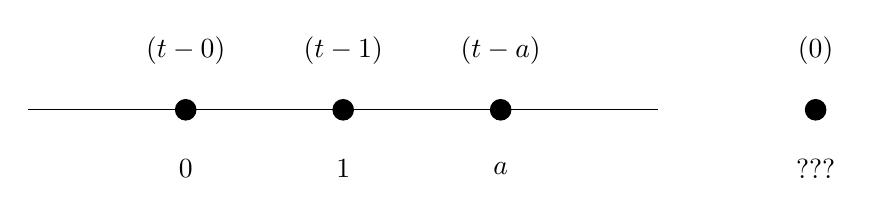
\begin{tikzpicture}[scale=1]
  \draw (0,0)--(8,0);
  \filldraw (2,0) circle (.13);
  \filldraw (4,0) circle (.13);
  \filldraw (6,0) circle (.13);
  \filldraw (10,0) circle (.13);

  \node at (2,.75) {$(t-0)$};
  \node at (4,.75) {$(t-1)$};
  \node at (6,.75) {$(t-a)$};
  \node at (10,.75) {$(0)$};
  
  \node at (2,-.75) {$0$};
  \node at (4,-.75) {$1$};
  \node at (6,-.75) {$a$};
  \node at (10,-.75) {???};
\end{tikzpicture}\]
A few things to note:
\begin{itemize}
\item At each point $(t-a)$ of the spectrum, we have an evaluation map
\begin{align*}
\C[t] &\to \frac{\C[t]}{(t-a)} \cong \C\\
f(t) &\mapsto f(a)
\end{align*}
That is, $f$ is sent to its image in $\C[t]/(t-a)$, which says $t$ can be swapped for $a$. That is, we send $f(t)$ to $f(a)$. This evaluates the polynomial at $a$. We will see a similar construction in general. Note that this means these points are keeping track of all the values of this function. If we have two different polynomials $f_1,f_2$ then their evaluations at some points will differ: i.e. functions are distinguished by their values. \textbf{This will not always be true!}. See Example \ref{example:dualnumbers}.

\item $(0)$ is called "the generic point." It is "close" to every point, so it is "generically" on the line, but is not equal to any of the $(t-a)$. Some would choose to draw it as "fuzz" amongst the line. We will understand the generic point better when we understand the topology of $\spec A$. 
\item $\spec \C[t]$ will come to be known to us as the complex affine line, denote $\A^1_{\C}$.
\end{itemize}
\end{example}

\begin{example}[Don't say I never gave you an example that wasn't over $\C$!] Consider $A = \R[t]$. The prime ideals are of one of two forms:
\[(t-a) \ \ a \in \R \quad \quad \quad (t-a)(t-\overline{a}) \ \ a \in \C \setminus \R\]
Hence we get an identification:
\[\spec \R[t] = \C/\textup{Gal}(\C/\R) \sqcup \{(0)\}\]
which you can identify with the upper half plane along with a generic point.
\end{example}

\begin{definition}[Evaluation map] Given a ring $A$, $f \in A$, and $\pp \in \spec A$, the \textbf{value of $f$ at $\pp$}, denoted by $f(\pp)$, is the image of $f$ under:
\[A \mapsto A/\pp \to \textup{Frac}(A/\pp)\]
This gives us a way to "evaluate" our sections/functions on points, but note that the field in which the values lie is thought of as varying with $\pp$. The field $\textup{Frac}(A/\pp) =: k(\pp)$ is known as the residue field at $\pp$.
\end{definition}

\begin{example}[Functions are not always separated by \textit{values} at points]\label{example:dualnumbers} Consider the set $\spec \C[t]/(t^2)$. As a set of points it has just one element: $(t)$.

$t$ is an element of the ring $\C[t]/(t^2)$, and we should think of it as being very small: so small that its square is zero, but it itself is not zero. If we think about the evaluations of this function note that:
\begin{align*}
\C[t]/(t^2) &\to \textup{Frac}(\C[t]/(t,t^2)) \cong \C\\
t & \mapsto 0
\end{align*}
That is, both the function $t$ and $0$ on the LHS evaluate to 0 on the RHS.But this is the only evaluation map to consider on this spec. So, we see how functions cannot be necessarily be separated by values. Eventually, we will see that the issue is that $\spec \C[t]/(t^2)$ is not \textit{reduced}. See Definition \ref{def:scheme-adj}.
\\

When drawing $\spec \C[t]/(t^2)$, one should visualize it as a point with a small tangent direction attached.
\end{example}

\hrule
\vspace{1em}

Now, it is time to define the topology on these spaces. The idea: closed sets should be sets of points where functions vanish (similar to 552).
\begin{align*}
f \textup{ vanishes at } \pp &\iff f(\pp) = 0 \\
& \iff f = 0 \textup{ in } A/\pp\\
&\iff f \in \pp \quad (\iff (f) \subseteq \pp)
\end{align*}

\begin{definition}[Various vanishing loci definitions] Let $f \in A$, $S \subseteq A$. Then:
\begin{align*}
V(f) &= \{\pp \in \spec A: (f) \subseteq \pp\}\\
V(S) &= \{\pp \in \spec A : S \subseteq \pp\} = \{\pp \in \spec A : \langle S \rangle \subseteq \pp\}
\end{align*}
Note that $V(S) = V(\langle S \rangle)$.
\end{definition}

\begin{definition} A (Zariski) closed subset of $\spec A$ is any set of the form of a vanishing locus $V(\fraka)$ for $\fraka$ an ideal.
\end{definition}

\begin{proposition} The collection of Zariski closed subsets forms a topology on $\spec A$.
\end{proposition}
\begin{proof}
Observe:
\begin{align*}
\varnothing &= V((1))\\
\spec A &= V((0))\\
V(\fraka) \cup V(\frakb) &= V(\fraka \frakb)\\
\bigcap_{i \in I} V(\fraka_i) &= V\left( \sum_{i \in I} \fraka_i \right)
\end{align*}
\end{proof}
\begin{example} The closed sets in $\spec \C[t]$ are the whole space, the empty set, and 
\[V(f(t)) = V\big(((t-a_1) \dots (t-a_n))\big) = \cup_{i=1}^n V((t-a_i)) = \{(t-a_i) : 1 \le i \le n\}\]
i.e. finite collections of non-generic points.

Note that $\overline{\{(0)\}} = \spec \C[t]$. That is, the generic point is "close" to all other points, and "sits along the whole line."
\end{example}

\begin{definition} Define $D(f) = \spec A \setminus V((f))$. These open sets form a basis for the topology.
\end{definition}

\begin{proposition} Let $S$ be a multiplicative set. By studying the map $\varphi: A \to S^{-1}A$, $a \mapsto a/1$, this induces a bijection:
\[\{\textup{primes in $A$ with $\pp \cap S = \varnothing$}\} \longleftrightarrow \{\textup{primes in $S^{-1}A$}\}\]
\end{proposition}

We've motivated that $A$ should be thought of as the ring of algebraic functions over $\spec A$. Then, what should be the ring of functions on the open set $D(f)$? Well, since we're not working with the full spec, we should be able to invert things that don't vanish on the set. That is, things whose vanishing sets are squirreled away in $V(f)$, the set we are cutting out.

Set $\OO_{\spec A}(D(f)) = S^{-1}A$ where $S$ is the following multiplicative set:
\[S = \{g \in A: g(\pp) \ne 0 \textup{ for all }\pp \in D(f)\} = \{g \in A: V(g) \subseteq V(f)\}\]
This definition only depends on $D(f)$, not on $f$ itself. But luckily:

\begin{proposition} The natural map
\[A_f \to \OO_{\spec A}(D(f))\]
is an isomorphism.
\end{proposition}

\begin{lemma}\label{lemma:restriction-well-def} $D(f) \subseteq D(g)$ (that is, $V(g) \subseteq V(f)$) if and only if $f^n \in (g)$, if and only if $g$ is invertible in $A_f$.
\end{lemma}
\begin{proof}
$f^n \in (g) \iff \sqrt{(f)} \subseteq \sqrt{g} \iff$ the prime ideals containing $(f)$ are a superset of those containing $(g)$, which means $V(g) \subseteq V(f)$. Then $f^k = gm$, so $g$ is invertible in $A_f$. 
\end{proof}

That is, algebraic functions on $D(f)$ are obtained by inverting $f$. So, we have the makings of a \textit{structure sheaf}, i.e. a sheaf $\OO_{\spec A}$ where $\OO_{\spec A}(U)$ is the ring of algebraic functions on $U$. But we only have it on a distinguished basis. The question becomes: is this enough to determine the sheaf overall? Will we be able to do computations in the future/check nice properties by just checking it on the basis of the $D(f)$? The answer: yes! Back to sheaf theory.
%#######################################################################
%#######################################################################
%####################    L E C T U R E      0 3  ###############################
%#######################################################################
%#######################################################################
\section{Jan 17: Let's understand sheaves better (stalks, morphisms)}
\textbf{Recommended reading: Hartshorne II.1,Vakil 2.3-2.4}

We learned about the topological spaces that will be glued into schemes. These are the $\spec A$, and we think of $A$ as the ring of algebraic functions on $\spec A$. Again, we want to assemble a structure sheaf $\OO_{\spec A}$ on $\spec A$ such that
\[\OO_{\spec A}(U) = \textup{ ring of algebraic functions on $U$}\]
From this perspective, we saw it was reasonable to set 
\[\OO_{\spec A}(D(f)) = S^{-1}A \cong A_f\]
where 
\[S = \{g \in A: g(\pp) \ne 0 \textup{ for all }\pp \in D(f)\} = \{g \in A: V(g) \subseteq V(f)\}\]

\textbf{Problem: what about this would-ve sheaf on open sets in general?} We would like to describe this sheaf, i.e. describe the rings of algebraic functions, on nice $D(f)$ to be enough. It is, but we need to do a bit of work to say that. (Here Vakil and Harthsorne somewhat "diverge." Vakil shows that defining a sheaf on a basis is sufficient; Hartshorne just describes the $\OO_{\spec A}(U)$ from the get-go, with the construction being the one you'd do when defining a sheaf from a base. In the end, they are equivalent data/constructions).
\\

We'll get to all that, but we should cover some necessary details/definitions/general knowledge first.
\\

\hrule
\vspace{1em} 

\begin{definition} Let $(X,\FF)$ be a sheaf on a topological space $X$. Let $x \in X$ be a point. The \textbf{stalk} of $\FF$ at $x$ is defined as the direct limit:
\[\FF_x := \varinjlim_{U \ni x} \FF(U) = \{(f,U) : f \in \FF(U), x \in U\}\]
where $(f,U) \sim (g,V)$ if and only if there is some $W \subseteq U,V$, with $W$ containing $p$, such that $f|_W = g|_W$.
\end{definition}

You can draw a pic of this in the case of the sheaf of differentiable functions on some differentiable manifold $M$. Equality on the stalk means two functions, defined near at point $x$, agree on some smaller open set around the point. Observe that in this case, the stalk is a local ring: its unique maximal ideal is the ideal of all functions vanishing at $x$.

\begin{definition} Elements of a stalk are called \textbf{germs}.
\end{definition}

\begin{definition} Given a section $f \in \FF(U)$ and a point $p \in U$, we let $f_p$ denote the image of $f$ in the stalk:
\begin{align*}
\FF(U) &\to \FF_p\\
 f &\mapsto f_p = (f, U)
\end{align*}
\end{definition}

\begin{remark} We will see later on that many properties we want to test of sheaves (or morphisms of sheaves) can be tested by checking the analogous condition on the stalks. This is reasonable, looking at the gluing axiom of a sheaf.
\end{remark}

\begin{definition}[Morphisms of (pre)sheaves] Let $\FF,\GG$ be (pre)sheaves on a topological space $X$. A morphism $\FF \to \GG$ is a collection of maps $\phi_U: \FF(U) \to \GG(U)$ for each $U$ such that the following diagram commutes:
\[\begin{tikzcd}
\FF(U) \arrow[r, "\phi_U"] \arrow[d, swap, "\res^U_V"]& \GG(U) \arrow[d, "\res^U_V"]\\
\FF(V) \arrow[r,"\phi_V"]& \GG(V)
\end{tikzcd}\]
Consequently, we can see that $\varphi$ defines a map on stalks $\varphi_x: \FF_x \to \GG_x$ by sending $(f,U) \to (\varphi_U(f),U)$. An isomorphism is a morphism with a two-sided inverse.
\end{definition}

Let's restrict our attention to sheaves of abelian groups at this point (we rarely fall outside this scenario).

\begin{proposition} Let $\FF,\GG$ be sheaves of abelian groups on a topological space $X$. Let $\varphi: \FF \to \GG$ be a morphism of sheaves. Then $\varphi$ is an isomorphism if and only if $\varphi_x$ is an isomorphism for all $x \in X$.
\end{proposition}
\begin{proof}\text{ }
$\Rightarrow$ is clear. We prove the $\Leftarrow$ direction. It is enough to show that $\varphi_U$ is an isomorphism for each $U$.

Let's start by showing injectivity: suppose $s \in \FF(U)$ is a section such that $\varphi_U(s) = 0$ in $\GG(U)$.  Then the germ $\varphi_U(s)_x = \varphi_x(s_x)$ is zero for each $x \in U$. Then $s_x = 0$ in each $x \in U$ by injectivity on stalks. Then it follows from the definition of the stalks that we can find an open cover of $U$ such that $s$ restricts to zero on each piece. That is, $s=0$.

Now we show surjectivity: suppose we are considering $\varphi_U : \FF(U) \to \GG(U)$. Let $t \in \GG(U)$. We'll piece together something that maps to it.

For each $x \in U$, we have $t_x \in \GG_x$ and it must be the image of some $s_x \in \FF_x$. $s_x$ can be repped by some $s(x) \in V_x \ni x$. Then $\varphi(s(x)), t|_{V_x}$ are two elements of $\GG(V_x)$ with the same germ, so $\varphi(s(x)), t$ agree in some neighborhood $W_x$ of $x$.

Cover $U$ with these $W_x$, and consider the $s(x)$ (well, technically $s(x)|_{W_x}$) that we get for each one. On the overlaps, these must agree due to injectivity (their overlaps go to $t|_{W_x}$). So we can piece them together to get an $s \in \FF(U)$ that maps to t.
\end{proof}

\begin{remark} Note that the proof of surjectivity needed injectivity!
\end{remark}

\begin{definition}[(\underline{Tentative} definition of ker, image, coker)] Given a morphism $\varphi: \FF \to \GG$ of presheaves of abelian groups, we can define the \underline{presheaves} $\ker(\varphi), \textup{coker}(\varphi), \textup{im}(\varphi)$, as follows:
\begin{align*}
\ker(\varphi)(U) &= \ker(\varphi_U: \FF(U) \to \GG(U)) \quad [\subseteq \FF(U)]\\
\textup{coker} (\varphi)(U) &= \textup{coker}(\varphi_U: \FF(U) \to \GG(U)) \\
\textup{im}\varphi)(U) &= \textup{im}(\varphi_U: \FF(U) \to \GG(U)) \quad [\subseteq \GG(U)]\\
\end{align*}
\end{definition}

\begin{proposition} Given $\varphi: \FF \to \GG$ a morphism of sheaves on $X$, the kernel is a sheaf
\end{proposition}
\begin{proof} Identity is inherited from the parent sheaf. Gluing is too, though you need to check that the glued function $f$ is still in the kernel. This works because $\varphi(f)$ restricts to zero on a cover, thus is zero globally from gluing in $\GG$.
\end{proof}

\begin{remark} Since we can view each $\ker(\FF)(U)$ as a subgroup of $\FF(U)$, we can think of $\ker(\FF)(U)$ as a \textit{subsheaf} of $\FF(U)$.
\end{remark}

\begin{proposition} The image and cokernel of a sheaf morphism need not be a sheaf
\end{proposition}
\textit{For the cokernel:} Let $X = \C$, and $\OO$ be the sheaf of holomorphic function and $\OO$ be the sheaf of nonzero holomorphic functions. Consider the map $\varphi$ with
\begin{align*}
\varphi_U: \OO(U) &\to \OO^*(U)\\
f & \mapsto e^f
\end{align*}
we claim that the cokernel isn't a sheaf. First, note that there is no holomorphic $f$ such that $e^f = z$ on $\C \setminus \{0\}$. Otherwise, differentiating both sides yields:
\[e^f \cdot f' = 1 \Rightarrow z \cdot f' = 1 \Rightarrow f' = 1/z\]
Integrating the LHS over a loop around zero yields $0$, but integrating the RHS over said loop produces $2\pi i$. Contradiction.

Therefore, $[z] \ne 0$ in $\textup{coker}(\varphi)$. That is, $\Gamma(\C \setminus \{0\}, \textup{coker}(\varphi)) \ne 0$. But, take $U_1 = \C \setminus (-\infty,0]$ and $U_2 = \C \setminus [0, \infty)$. These are simply connected, so every nonzero function on them can be writting as some $e^f$ (we can define the log: we made a branch cut!). Thus $\coker(\varphi)(U_1), \coker(\varphi)(U_2)$ are both zero. So the cokernel fails the identity axiom.

Similarly, this shows why the image isn't necessarily a sheaf: we can't glue the logs of $z$ into a log of $z$ on all of $\C \setminus\{0\}$.
\\

\hrule
\vspace{1em}

So, we have all these presheaves running around (including ones we'd really like to consider: the image and cokernel are imporant!). We would like some way to modify them into a sheaf, and it should have some nice universal property that relates it back to the original presheaf.

\begin{construction}[Sheafification] Given a presheaf $\FF$, there is a sheaf $\FF^{+}$ and a morphism $\theta: \FF \to \FF^+$ with the property that: for any sheaf $\GG$ and any morphism $\varphi: \FF \to \GG$, there is a unique morphism $\varphi^+$ such that $\varphi = \varphi^+ \circ \theta$. The pair $(\FF^+, \theta$ is unique up to unique isomorphism.
\[\begin{tikzcd}
\FF \arrow[dr, "\varphi"] \arrow[r, "\theta"]& \FF^+ \arrow[d, dashed,"\varphi^+"]\\
& \GG
\end{tikzcd}\]
\end{construction}
%#######################################################################
%#######################################################################
%####################    L E C T U R E      0 4  ###############################
%#######################################################################
%#######################################################################
\section{Jan 22: Sheafifcation, sheaves on a base}
\textbf{Recommended reading: Harthsorne II.1 ($\sim$ p. 64), Vakil 2.4-5}

Recall: last time we saw how some ker, coker of morphism of sheaves was not necessarily a sheaf. This motivates sheafification, which will also set us up well for doing \textit{sheaves on a base}, which will help us define the structure sheaf on $\spec A$.

Now, for the construction of the sheafification of a presheaf. The construction is: bundle the stalk data in a nice way. That is, make a big product of the stalks, but only allow combinations of germs that looked like they could glue together.

\begin{align*}
\FF^+(U) &:= \left\{(f_p)_{p \in U} : \begin{array}{l} \textup{ for all $p \in U$, there is an open $V$ with $p \in V \subseteq U$} \\ \textup{and an $s \in \FF(V)$ such that $s_q = f_q$ for all $q \in V$}\end{array}\right\}\\
& \subseteq \prod_{p \in U}\FF_p
\end{align*}
the morphism $\theta$ is clear: $\theta_U$ is $f \mapsto (f_p)_{p \in U}$. To describe $\varphi^{+}$: look at the sections that glue to your $(f_p)$, look at their images, glue them in the target, and call that the image. This is unique: in order for the diagram to commute any other map would have to do the same thing.

\begin{remark} Sheafification is a functor from presheaves on $X$ to sheaves on $X$.
\end{remark}

\begin{remark} Specifically, given $i: \textup{Shf}_X \to \textup{Pre}_X$ the inclusion map from sheaves on $X$ to presheaves on $X$, note that sheafification is  $+: \textup{Pre}_X \to \textup{Shf}_X$. Then $+$ is the left adjoint of $i$, i.e. given $\FF$ a sheaf on $X$ and $\GG$ a presheaf on $X$, we have the natural bijection:
\[\Hom_{\textup{Pre}_X} (\GG, i(\FF)) \cong \Hom_{\textup{Shf}_X}(\GG^+, \FF)\] 
\end{remark}

\begin{example}[Constant sheaves] Let $X$ be a topological space, $S$ a set. You get the constant presheaf by assigning the same set to all open sets:
\[\FF(U) = S\]
(On nonempty sets, you can interpret this as constant functions from $U$ to $S$). Gluing is a mess because of disjoint sets, and the empty set presents problems too: all sections in $\FF(\varnothing)$ restrict to the same thing on the empty cover. So the identity axiom says all sections on $\varnothing$ ought to be the same.

The sheafification $\FF(U)$ will instead assign to $U$: locally constant maps from $U$ to $S$. Denote this sheaf as $\underline{S}$.
\end{example}

\begin{remark} Thinking of sheaves of abelian groups: sheafification adds the gluings that should exist but don't, and kills off the nonzero sections that are locally zero.
\end{remark}

\begin{proposition} $\FF \to \FF^+$ yields an isomorphism of stalks.
\end{proposition}
\begin{proof} Work from the explicit description.
\end{proof}

\hrule
\vspace{1em}

\begin{definition} We say that a map of sheaves is injective if and only if the kernel sheaf is zero.
\end{definition}

\begin{lemma} A map of sheaves if injective $\iff \varphi: \FF(U) \to \GG(U)$ is injective for each $U$. Likewise, it is injective $\iff$ it is injective on stalks.
\end{lemma}
\begin{proof}
This was done in the bijectivity proof before.
\end{proof}

\begin{definition} We define the image and cokernel \textit{sheaves} by taking the sheafification of the presheaves defined above. We generally just call them $\textup{im}(\varphi)$ and $\textup{coker}(\varphi)$ and drop any $+$ notation, and usually refer to the presheaf versions as $\textup{im}(\varphi)^{\textup{pre}}, \textup{coker}(\varphi)^{\textup{pre}}$.
\end{definition}

\begin{remark} Consider a map of sheaves $\varphi: \FF \to \GG$ on $X$. Since we have a map $\textup{im}^{\textup{pre}}(\varphi) \to \GG$, we necessarily have a map $\textup{im}(\varphi) \to G$. This map is injective: it is injective on the level of stalks (note that the presheaf and sheafified image have the same stalks!). Thus, we can identify $\textup{im}(\varphi)$ with a subsheaf of $\GG$.
\end{remark}

\begin{definition} A morphism of sheaves $\varphi: \FF \to \GG$ is surjective if $\textup{im}(\varphi) = \GG$.
\end{definition}

\begin{lemma} $\varphi: \FF \to \GG$ is surjective if and only if $\FF_x \to \GG_x$ is surjective for all points $x$.
\end{lemma}
\begin{proof}\text{ }
$\Leftarrow$: $\im(\FF) = \GG$ means the stalks are isomorphic, hence $\FF_x \to \GG_x$ must be surjective.

$\Rightarrow$: we want to show that $\im(\FF) = \GG$. Well, the map on stalks is an isomorphism (injective and surjective on stalks), so they are equal.
\end{proof}

\begin{example} In our example with $X = \C$, $\OO_X$ the sheaf of holomorphic functions, and $\OO_X^*$ the sheaf of non-vansihing holomorphic functions and 
\begin{align*}
\OO_X &\to \OO_X^*\\
f &\mapsto e^f
\end{align*}
we have that $\im(\varphi) = \OO_X^*$ and $\coker(\varphi) = 0$. This can be seen via $\varphi$ being surjective on the level of stalks (and correspondingly the cokernel is zero on the level of stalks).
\end{example}

\begin{definition} A sequence of maps
\[\FF^{i-1} \stackrel{\varphi^{i-1}}{\to} \FF^i \stackrel{\varphi^i}{\to} \FF^{i+1}\]
is exact if at each stage, $\ker \varphi^{i} = \im \varphi^{i-1}.$
\end{definition}
%#######################################################################
%#######################################################################
%####################    L E C T U R E      0 5  ###############################
%#######################################################################
%#######################################################################
\section{Jan 24: Sheaves on a base, affine schemes}
\textbf{Recommended reading: Vakil 2.5, 4.1}

Time to handle an issue: sometimes we understand a sheaf really well on a nice basis. But what about the rest? The details are sometimes unpleasant/obfuscating: it is mainly important to know that the data of the sheaf on a suitably nice basis is enough to determine the sheaf. The construction will be reminiscent of sheafification.

\begin{definition} A base of a topology is a collection of open sets $\{B_j\}_{j \in J}$ such that any open set of $X$ can be written as a union of $B_j$.
\end{definition}

\begin{remark} $(f) \subseteq \fraka \iff V(f) \supseteq V(\fraka) \iff D(f) \subseteq D(\fraka)$, so the $D(f)$ genuinely are a basis of the Zariski topology on $\spec A$.
\end{remark}

\begin{definition} Suppose $\{B_i\}$ is a basis on $X$. A presheaf of sets on the base if an assignment $F(B_i)$ for each $B_i$. If $B_j \subseteq B_i$, we have restriction maps $\res^{B_i}_{B_j}$ satisfying $\res^{B_i}_{B_i} = \textup{id}$ and $\res^{B_i}_{B_k} = \res^{B_j}_{B_k} \circ \res^{B_i}_{B_j}$. 

For sheaves on a base: there are base identity and base gluing axioms:
\begin{itemize}
\item If $B \in \{B_i\}$ can be written as $B = \cup_{i \in J} B_i$ and $f,g \in F(B)$ with $\res^B_{B_i} f = \res^B_{B_i} g$ for all $i \in J$, then $f=g$.
\item If we have $f_i \in B_i$ for $i \in J$ such that for any $i,j$ we have $\res^{B_i}_{B_k} f_i = \res^{B_i}_{B_k} f_j$ for any $B_k \subseteq B_i \cap B_j$, then there is an $f \in F(B)$ such that $f|_{B_i} = f_i$ for all $i \in J$.
\end{itemize}
\end{definition}

\begin{theorem} Suppose $\{B_i\}$ a base on $X$, and $F$ a sheaf of sets on this case. There is a sheaf $\FF$ extending $F$ ($\FF(B_i) \cong F(B_i)$ with isomorphisms agreeing with restriction maps). $\FF$ is unique up to unique isomorphism.
\end{theorem}
\begin{proof}
As before, $\FF$ is a sheaf of compatible germs. Define the stalk of a presheaf $F$ on a base as:
\[F_p = \varinjlim_{B_i \ni p} F(B_i)\]
Define
\begin{align*}
\FF(U) &:= \left\{(f_p \in F_p)_{p \in U} : \begin{array}{l} \textup{ for all $p \in U$, there is a $B$ with $p \in B \subseteq U$} \\ \textup{and an $s \in \FF(B)$ such that $s_q = f_q$ for all $q \in B$}\end{array}\right\}\\
& \subseteq \prod_{p \in U}F_p
\end{align*}
We get a map $F(B) \to \FF(B)$ for each $B$, which is an isomorphism. Checking the details is similar to the work for sheafificiation.

Note that clearly $\FF_p \cong F_p$.
\end{proof}

\hrule
\vspace{1em}

We can finally really talk about the structure sheaf on $\spec A$. Consider $\spec A$ with the Zariski topology, and for open sets $D(f)$ set
\[\OO_{\spec A}(D(f)) = S^{-1}A \cong A_f\]
 where $S = \{g \in A: g(\pp) \ne 0 \textup{ for all }\pp \in D(f)\} = \{g \in A: V(g) \subseteq V(f)\}$. The restriction maps are clear enough: if $D(g) \subseteq D(f)$ then the restriction map
 \[\res^{D(f)}_{D(g)}: \OO_{\spec A}(D(f)) \to \OO_{\spec A}(D(g))\]
 is further localization. This is clearly a presheaf on a distinguished base.
 
 \begin{lemma} $\spec A$ is quasi-compact (every open cover has a finite subcover).
 \end{lemma} 
 \begin{proof} It's enough to show this for covers for the form $\{D(f_i)\}$. Note that $\cup D(f_i) = D(\sum (f_i))$. This will be all of $\spec A$ only when $1 \in sum (f_i)$, in which case we get $1 = a_{i_1}f_{i_1} + \dots + a_{i_k}f_{i_k}$ and you can just take the corresponding cover pieces $D(f_{i_1}), \dots, D(f_{i_k})$.
 \end{proof}
 
 \begin{theorem} This assignment of $\OO_{\spec A}(D(f))$ gives a sheaf on a distinguished base, and thus determines a sheaf on $\spec A$. This sheaf is the \textbf{structure sheaf} on $\spec A$, and is referred to as $\OO_{\spec A}$ or just $\OO$ if it is clear what $A$ is.
 \end{theorem}
 \begin{proof} It's enough to show identity and gluing on just $A$ (if you want to show it on $D(f)$, that's the same as swapping the ring out for $A_f$, modulo some detail-checking).
 \begin{itemize}
 \item \textbf{Identity axiom}: Write $\spec A = \cup_i D(f_i)$. Then after potentially relabeling, we can pick a finite subcover. Write $\spec A = \cup_{i=1}^n D(f_i)$. That is, $V((f_1,\dots,f_n)) = \varnothing$, i.e. $(f_1,\dots,f_n) = A$.
 
 Suppose we have a section $s \in \OO_{\spec A}(\spec A) = A$ such that $\res^{\spec A}_{D(f_i)} s= 0 \in A_{f_i}$ for each $f_i$. That means there is some $m$ such that $f_i^m s = 0$ (in $A$) for $1 \le i \le n$. 
 
 But note that $D(f_i) = D(f_i^m)$ (as $f_i$ vanishes at $\pp$ if and only if $f_i^m$ vanishes at $\pp$). So there are $g_i$ such that 
 \[1 = \sum_{i=1}^n g_i f_i^m\]
 But then:
 \[s = \sum_{i=1}^n g_i f_i^m s = \sum 0 = 0\]
 \item \textbf{Gluing}: Again, being able to write $1$ as a sum of these $f_i$ will let us piece things together in a nice way.
 
 Again, say we have some gluing data on an open cover. Pick a finite subcover $\{D(f_i)\}_{i=1}^n$. Let $s_i \in \OO_{\spec A}(D(f_i))$ so that
 \[\res^{D(f_i)}_{D(f_i) \cap D(f_j)} s_i = \res^{D(f_j)}_{D(f_i) \cap D(f_j)} s_j \]
 noting that $D(f_i) \cap D(f_j) = D(f_if_j)$. Identifying $\OO_{\spec A}(D(g))$ with $A_g$, we get that 
 \[s_i = \frac{a_i}{f_i^{\ell_i}}, \quad s_j = \frac{a_j}{f_j^{\ell_j}}\]
 and because their restrictions are the same in $A_{f_if_j}$, it must be that there is an $m_{i,j}$ such that
 \[(a_if_j^{\ell_j} - a_j f_i^{\ell_i})(f_i f_j)^{m_{i,j}} = 0.\]
 Let $m = \max m_{i,j}$. Then the above tells us that:
 \[(a_i f_i^m) f_j^{m + \ell_j} = (a_j f_j^m) f_i^{m + \ell}.\]
 Now again, $\spec A = \cup D(f_i^{m + \ell_i})$, so there exists $g_i \in A$ such that
 \[1 = g_1f_1^{m+ \ell_1} + \dots g_n f_n^{m+\ell_n}\]
 and consider the element of $A$ given by:
 \[s = g_1a_1f_1^{m} + \dots g_n a_nf_n^{m}\]
 Then observe that:
 \begin{align*}
 f_i^{m+\ell_i} s &= g_1(a_1 f_1^m)f_i^{m+\ell_i} + \dots + g_n(a_n f_n^m)f_i^{m+\ell_i}\\
 &= g_1f_1^{m+\ell_1}(a_if_i^m) + \dots + g_n f_n^{m+\ell_n}(a_if_i^m)\\
 &= ( g_1f_1^{m+ \ell_1} + \dots g_n f_n^{m+\ell_n})a_i f_i^m\\
 &= a_i f_i^m
 \end{align*}
 That is, $f_i^m(f_i^{\ell_i}s - a_i) = 0$. That is, $s = \frac{a_i}{f_i^{\ell_i}} = s_i$ on $A_{f_i}$, which is what we wanted.
 
 You can use the identity axiom proved prior to show that the resulting glued object restricts to what you want on the other elements of the a priori infinite cover. So the identity proof does need to come first!
 \end{itemize}
 \end{proof}
 Thus, we can finally start talking about affine schemes.
%#######################################################################
%#######################################################################
%####################    L E C T U R E      0 6  ###############################
%#######################################################################
%#######################################################################
\section{Jan 27: Affines schemes, schemes}
\textbf{Recommended reading: Hartshorne II.2, Vakil 4.1-4.4}

\begin{proposition} Let $A$ be a ring and $\OO$ the structure sheaf on $\spec A$. For any $\pp \in \spec A$, the stalk $\OO_{\pp} \cong A_{\pp}$.
\end{proposition}
\begin{proof}
Fairly evident from the description of $A_{\pp}$ as  a direct limit identifying a bunch of subsequent localizations. For $f \not \in \pp, D(f)$ will appear in the direct limit. Lemma \ref{lemma:restriction-well-def}  can help. To be more concrete, we can write down the map.

And $(s,D(f)) \in \OO_{\pp}$ can be sent to its image in $A_{\pp}$. It is surjective: any element in $A_{\pp}$ is of the form $a/g$ for $g \not \in \pp$, and so $\pp \in D(g)$. That is, $D(g)$ will be a neighborhood of $\pp$ and $a/g$ will be hit by the map.

It is injective: write $s = a/f, t = b/g$, with $f,g \not \in \pp$. These are sections on $D(f), D(g)$ respectively. If their image is the same in $A_{\pp}$, then there is some $h \not \in \pp$ such that $h(ga-fb) = 0$ in $A$. But then $D(fgh) = D(f) \cap D(g) \cap D(h)$ is a neighborhood of $\pp$ and so $s,t$ (after restriction to $D(fgh)$) would have been identified in the stalk $\OO_p$.
\end{proof}

Now, we need some way to compare or relate sheaves on different spaces. This necessitates the direct image and inverse image functors.

\begin{definition} Let $f: X \to Y$ be a continuous map of topological spaces. Let $\FF$ be a sheaf on $X$. The \textbf{direct image} sheaf $f_* \FF$ on $Y$ is defined via
\[(f_* \FF)(V) = \FF(f^{-1}(V))\]
for open sets $V \subseteq Y$. This is a functor from sheaves on $X$ to sheaves on $Y$.
\end{definition}

\begin{definition}
Let $f: X \to Y$ a continuous map of topological spaces and $\GG$ a sheaf on $Y$. The \textbf{inverse image} sheaf $f^{-1}\GG$ on $X$ is the sheafification of the presheaf:
\[U \mapsto \varinjlim_{V^{\textup{open}} \supseteq f(U)} \GG(V).\]
This is a functor from sheaves on $Y$ to sheaves on $X$.
\end{definition}

\begin{definition}
If $i: Z \to X$ is a subset of $X$ with the subspace topology, then $i^{-1}\FF$ is the restriction of $\FF$ to $Z$, denoted by $\FF|_{Z}$. For open sets $Z$ this will just turn into $\FF|_{Z}(V) = \FF(V)$.
\end{definition}

\begin{definition} A \textbf{ringed space} is a pair $(X,\OO_X)$ of a topological space $X$ and a sheaf of rings on $X$. A morphism of ringed spaces $(X,\OO_X) \to (Y,\OO_Y)$ is a pair $(f,f^{\sharp})$ of a continuous map $f: X \to Y$ and a morphism of sheaves (of rings) $f^{\sharp}: \OO_Y \to f_* \OO_X$.

A ringed space $(X,\OO_X)$ is a \textbf{locally ringed space} if all the stalks $\OO_{X.p}$ are local rings. A morphism of locally ringed spaces is a morphism of ringed spaces such that the induced map on stalks $f_p^{\sharp}: \OO_{Y, f(P)} \to \OO_{X,P}$ is a local homomorphism of local rings.

Here, a local homomorphism of local rings $\varphi: A \to B$ is a ring morphism such that $\varphi^{-1}(\frak{m}_B) = \frak{m}_A$. An isomorphism is a morphism (of ringed or locally ringed spaces respectively) with a two-sided inverse. Equivalently, in $(f,f^{\sharp})$ the $f$ is a homeomorphism and the $f^{\sharp}$ is an isomorphism of sheaves.
\end{definition}

\begin{remark} The induced map on stalks comes from:
\[\OO_{Y,f(P)} = \varinjlim_{V \ni p} \OO_Y(V) \to \varinjlim_{f^{-1}(V)} \OO_X(f^{-1}(V)) \to \varinjlim_{U \ni p} \OO_X(U) = \OO_{X,P}\]
\end{remark}

\begin{proposition}\text{ }
\begin{enumerate}[(a)]
\item $(\spec A, \OO_{\spec A})$ is a locally ringed space.
\item $\varphi: A \to B$ a morphism of rings induces
\[(f,f^{\sharp}) : (\spec B, \OO_B) \to (\spec A, \OO_A)\]
\item In fact, any morphism of locally ringed spaces $(\spec B, \OO_B) \to (\spec A, \OO_A$ is induced by a homomorphism of rings.
\end{enumerate}
\end{proposition}
\begin{proof}\text{ }
\begin{enumerate}[(a)]
\item Immediate from previous results.
\item The map on topological spaces is $f(\pp) = \varphi^{-1}(\pp)$. $f^{-1}(V(\fraka)) = V(\varphi(\fraka))$ so the map in continuous. Two ways to see the induced morphism on structure sheaves:
\begin{itemize}
\item  Certainly we yield a morphism on a base 
\[\OO_A(D(f)) \to \OO_B(D(\varphi(f)) = \OO_B(f^{-1}(D(f)) = f_*(\OO_B)(D(f))\]
via $A_f \to B_{\varphi(f)}$ in the obvious way, and it respects restriction maps.
\item Localize at each prime to get a local homomorphism of loca rings $\varphi_{\pp}: A_{\varphi^{-1}(\pp)} to B_{\pp}$. Since sheaves are isomorphic to their sheafification, you can interpret sections on $U$ as collections of compatible germs, and so you can just map germs (and compatibility is preserved).
\end{itemize}
\item Take global sections: we must have a map:
\[\varphi: \OO_A(\spec A) \cong A \to \OO_{\spec B}(\spec B) \cong B\]
One can show that $\varphi$ induces all of the data of the morphism. Notably, we must have an induced morphism on stalks: $A_{f(\pp)} \to B_{\pp}$. Due to compatibility, we must have:
\[\begin{tikzcd}
A \arrow[d] \arrow[r,"\varphi"] & B \arrow[d]\\
A_{f(\pp)} \arrow[r, "f^{\sharp}_{\pp}"]& B_{\pp}
\end{tikzcd}\]
Since $f^{\sharp}_{\pp}$ is a local homomorphism, it must be that $\varphi^{-1}(\pp) = f(\pp)$, so that map $f$ on points coincides with the one induced by $\varphi$. Then compatibility with restriction maps will force the $f^{\sharp}$ to be induced by $\varphi$ as well.
\end{enumerate}
\end{proof}

\begin{definition} An \textbf{affine scheme} is a locally ringed space $(X,\OO_X)$ that is isomorphic, as a locally ringed space, to some $(\spec A, \OO_{\spec A})$.

A \textbf{scheme} is a locally ringed space $(X,\OO_X)$ such that every point $p \in X$ has an open neighborhood $U$ such that $(U,\OO_X|_U)$ is an affine scheme.
\end{definition}

\begin{example}[Schemes can be glued] Let $X_1,X_2$ be schemes. Let $U_i \subseteq X_i$ be open sets. Let $\varphi: (U_1, \OO_X|_{U_1}) \to (U_2, \OO_{X}|_{U_2})$ be an isomorphism of locally ringed spaces.

Then we can defined a scheme $X$ obtained by gluing $X_1,X_2$ by identifying $U_1,U_2$ via the morphism $\varphi$. The topological space is the quotient of $X_1 \sqcup X_2$ by the equivalence relation $x_1 \sim \varphi(x_1)$ for each $x_1 \in U_1$. The space is endowed with the quotient topology (a set is open $\iff$ its preimage is open).

We get maps $i_j: X_j \to X$ and the structure sheaf is defined as:
\[\OO_X(V) = \{(s_1,s_2) : s_j \in \OO_{X_j}(i_j^{-1}(V)), \ \   \varphi(s_1|_{i_1^{-1}(V) \cap U_1}) = s_2|_{i_2^{-1}(V) \cap U_2} \}\]
that is, sections on sets that "see" the overlap are gotten from piecing together compatible sections on (subsets of) each $X_1,X_2$.
\end{example}

\begin{example}[More concrete: the projective line] Recall that the morphisms of affine schemes are induced by ring morphisms on the globals ections. Glue $\spec \C[t]$ and $\spec \C[s]$ along $D(t) = \spec \C[t,t^{-1}] \cong \spec \C[s,s^{-1}] = D(s)$ via the following:
\[\begin{tikzcd}
\spec \C[s] & \spec \C[t]\\
\spec \C[s,s^{-1}] \arrow[u,"i_1"] \arrow[r]& \spec \C[t,t^{-1}] \arrow[u,"i_2"]
\end{tikzcd} \quad \quad \quad
\begin{tikzcd}
\C[s] \arrow[d]& C[t] \arrow[d] \\
\C[s,s^{-1}] &  \C[t,t^{-1}] \arrow[l, swap, "t \mapsto s^{-1}"] 
\end{tikzcd}\]
This yields the projective line. We will learn about the proj construction in general next lecture.
\end{example}

\begin{example}[What if you take the other transition function?] If we instead take the transition function as $t \mapsto s$:
\[\begin{tikzcd}
\spec \C[s] & \spec \C[t]\\
\spec \C[s,s^{-1}] \arrow[u,"i_1"] \arrow[r]& \spec \C[t,t^{-1}] \arrow[u,"i_2"]
\end{tikzcd} \quad \quad \quad
\begin{tikzcd}
\C[s] \arrow[d]& C[t] \arrow[d] \\
\C[s,s^{-1}] &  \C[t,t^{-1}] \arrow[l, swap, "t \mapsto s"] 
\end{tikzcd}\]
then this glues everything away from the origin in a "straightforward" way and we get the affine line with a doubled origin.
\end{example}
%#######################################################################
%#######################################################################
%####################    L E C T U R E      0 7  ###############################
%#######################################################################
%#######################################################################
\section{Jan 29: Proj, properties of schemes}
\textbf{Recommended reading: Hartshorne II.2 ($\sim$ 76-77), Vakil 4.5}

Now for the proj construction: we want a big class of examples from projective varieties, and we want a big class of interesting schemes in one fell swoop. An important tool is the notion of gluing schemes from more than two charts: the details are handled in Harthsorne exercise II.2.12. Note the cocycle condition on triple overlaps.

Intuition from 552 remains: if $S_{\bullet} = k[x_0,\dots,x_n]$, the proj construction yields $\PP^n_k$ and if $S_{\bullet} = k[x_0,\dots,x_n]/(f)$ where $f$ is homogeneous, we get something "cut out" of $\PP^n_k$ by the equation $f = 0$.

\begin{definition}[$\Z$-graded rings] A $\Z$-graded ring is a ring $S_{\bullet} = \oplus_{n \in \Z} S_n$ where multiplication respects grading: $S_m \times S_n \to S_{m+n}$. $S_0$ is a subring and each $S_n$ is an $S_0$ module, and $S_{\bullet}$ is an $S_0$ module. A $\Z^{\ge 0}$-graded ring is a $\Z$-graded ring with no elements of negative degree. We will, in the future, use graded ring to refer to a $\Z^{\ge 0}$ graded ring.
\end{definition}

\begin{definition} An element of some $S_n$ is a homogeneous element. If it is nonzero, nonzero, the subscript yields the degree.
\end{definition}

\begin{definition} An ideal $I$ of $S_{\bullet}$ is homogeneous if it is generated by homogeneous elements.
\end{definition}

\begin{proposition} An ideal is homogeneous if and only if it contains the degree $n$ piece of each of its elements.
\end{proposition}
\begin{proof}An induction proof by successively lopping off the top-degree pieces.
\end{proof}

\begin{definition} In a graded ring $S_{\bullet}$, the irrelevant ideal refers to $S_+ := \oplus_{i > 0} S_i$.
\end{definition}

\begin{definition} As a set, $\proj S$ is the set of all homogeneous prime ideals $\pp$ that do not contain all of $S_+$. For $\fraka$ a homogeneous ideal of $S$, we define the subset 
\[V(\fraka) = \{\pp \in \proj S: \fraka \subseteq \pp\}\]
For a set $T$, $V(T) = V((T))$. We have distinguished open sets (well, we will eventually see they're open) $D(f) := \proj S \setminus V((f))$ for $f$ homogeneous. Note that $D(fg) = D(f) \cap D(g)$.
\end{definition}

\begin{lemma} \text{ }
\begin{enumerate}[(a)]
\item For $\fraka, \frakb$ homogeneous ideals in $S$, we have $V(\fraka \frakb) = V(\fraka) \cup V(\frakb)$.
\item For any collection of homogeneous ideals $\{a_i\}$ of $S$, we have
\[V\left(\sum \fraka_i \right) = \bigcap V(\fraka_i)\]
\end{enumerate}
\end{lemma}
\begin{proof}
Same as before, accounting for the following: a homogeneous prime ideal $\pp$ is prime $\iff$ for two homogeneous $a,b \in S$, the product $ab \in \pp$ implies $a \in \pp$ or $b \in \pp$.
\end{proof}

Hence we can define a Zariski topology on $\proj S$. Now we must define a structure sheaf on this space. The idea: on the $D(f)$ we'd like the scheme to look like $\spec ((S_{\bullet})_f)_0$. Think about the standard affine opens on $\PP^n_k$ from 552, where the coordinate rings look like $k[x_0/x_i,\dots,x_n/x_i]$.

\begin{definition} For $f \in S_+$, set 
\[\OO_{\proj S_{\bullet}}(D(f)) = \OO(D(f)) = ((S_{\bullet})_f)_0 = "S_{(f)}"\]
See Hartshorne p. 76 or Vakil Section 4.5 if you want to see more on the details on issues relating to, e.g., whether restriction maps will make sense.
\end{definition}

\begin{proposition} Let $S$ be a graded ring.
\begin{enumerate}[(a)]
\item The stalk $\OO_{\pp}$ is isomorphic to the local ring $\SS_{\pp}$, the degree zero elements of $S$ localized at all \textbf{homogeneous} elements not in $\pp$.
\item We have that
\[D(f), \OO|_{D(f)} \cong \spec ((S_f)_0)\]
\item $\proj S$ is a scheme.
\end{enumerate}
\end{proposition}

It would do you well to read Exercise II.2.12 to get a sense of the work needed to glue together schemes.

\begin{example} For $A$ a ring, we get $\PP^n_A = \proj A[x_0,\dots,x_n]$, the projective $n$-space over $A$. For $A = k$ algebraically closed, you get something whose set of closed points is homeomorphic to the usual variety we know as projective $n$-space from 552.
\end{example}

\begin{definition} Let $S$ be a fixed scheme. A \textbf{scheme over $S$} is a scheme $X$ with a morphism $X \to S$. A morphism $X \to Y$ as schemes over $S$ is a morphism of schemes $f:X \to Y$ that is compatible with the morphisms to $S$. Then $\frak{Sch}(S)$ is the category of schemes over $S$. If $A$ is a ring, $\frak{Sch}(A)$ is the category of schemes over $\spec A$.
\end{definition}

\begin{proposition} Let $k$ be algebraically closed. There is a natural, fully faithful (that is, bijective on hom sets) functor $t: \frak{Var}(k) \to \frak{Sch}(k)$. For any variety, the topological space is homeomorphic to the set of closed points $\textup{sp}(t(V))$ and its sheaf of regular functions is obtained by restricting the structure sheaf of $t(V)$ via the homeomorphism.
\end{proposition}
\begin{proof}
See II.2, Proposition 2.6, of Harthshorne.
\end{proof}

\hrule
\vspace{1em}

Now it's time to think of all the interesting properties of schemes we could want:

\begin{definition}[Big list of scheme adjectives]\label{def:scheme-adj}Let $X$ be a scheme.
\begin{enumerate}[(a)]
\item $X$ is connected if its topological space is connected
\item $X$ is irreducible if the topological space is irreducible (all nonempty open sets dense).
\item $X$ is integral if all the $\OO_X(U)$ are integral domains
\item $X$ is reduced if all the $\OO_X(U)$ have no nilpotent elements (equivalently, by II.2.3, all the stalks have no nonzero nilpotents).
\end{enumerate}
\end{definition}

\begin{remark} At this point, it is useful to remark that the residue field of a point $\pp$ in a scheme $X$ is 
\[k(\pp) := \OO_{X,\pp}/m_{\pp}\]
This lines up with our old definition: if $\pp$ lies in an affine open $U \cong (\spec A,\OO_{\spec A})$, then $k(\pp) = \textup{Frac}(A/\pp)$. The presentation above has the advantage of not needing an affine chart to state it. Likewise, we have a notion of evaluation: for $f \in \OO_X(U)$, we have $f(\pp)$ is the image of $f$ under $\OO_X(U) \to \OO_{X,\pp}/m_{\pp} = k(\pp)$.

Note that for a section $f \in \OO_X(U)$, we have that $f_{\pp} \in \frak{m}_p \subseteq \OO_{X,\pp}$ is the same as $f(\pp) = 0$.
\end{remark}

\begin{proposition} A scheme is integral iff it is both reduced and irreducible.
\end{proposition}
\begin{proof} Integral certainly implies reduced. And if it's not irreducible, then it has two nonempty disjoint sets, yielding
\[\OO_X(U_1 \sqcup U_2) = \OO_X(U_1) \times \OO_X(U_2)\]
which is not integral.

Conversely: suppose $X$ is reduced and irreducible. Suppose there are $f,g \in \OO_X(U)$ with $fg = 0$. Then look at 
\begin{align*}
Y &= \{x \in U: f_x \in m_x\} = \{x \in U: f(x) = 0\}
Z &= \{x \in U: g_x \in m_x\} = \{x \in U: g(x) = 0\}
\end{align*}
These are closed subsets (exercise II.2.16 - on HW! Note that these are defined by vanishing conditions) of $U$, and $Y \cup Z = U$. But $X$ is irreducible, so $U$ is irreducible. So, then, say $Y = U$. But then $f$ is nilpotent on any affine open in $U$ (II.2.18a) meaning $f$ is zero.
\end{proof}

\begin{proposition} Suppose $X$ is a reduced scheme. Let $f,g \in \Gamma(X,\OO_X)$. Then:
\[f = g \iff f(x) = g(x) \textup{ (in $k(x))$ for all $x \in X$}\]
That is, evaluating the same everywhere means the two sections are the same.
\end{proposition}
\begin{remark} What this says is that, on reduced schemes, functions are determined by their values. Recall that the example of a setting where this is not true was $\spec k[x]/(x^2)$, which is certainly not reduced.
\end{remark}

\begin{proof}\text{ }
$\Rightarrow$: this direction is obvious.

$\Leftarrow$: We may assume $X$ is affine (you'll get equality on each open affine, and then glue to finish). In that case, $X = \spec A$ for $A$ with nilradical equal to $(0)$. We have:

\[A \to \prod_{\pp \in \spec A} \textup{Frac}(A/\pp) = \prod_{\pp \in \spec A} k(\pp) \quad \left(\textup{ equivalently, $A \hookrightarrow \prod_{\pp} \OO_{\spec A,\pp} \to \prod_{\pp} k(\pp)$}\right)\]
The kernel is the intersection of all prime ideals, which is $(0)$. That is, the map is injective. So since $f-g$ maps to zero, it must be that $f-g = 0$, and we are done.
\end{proof}

\begin{definition} A scheme is \textbf{locally noetherian} if it can be covered by open affine subsets $\spec A_i$ where each $A_i$ is notherian. $X$ is \textbf{noetherian} if it is locally noetherian and quasi-compact. Equivalently, $X$ is noetherian if it can be covered by a finite number of open affine subsets $\spec A_i$, each $A_i$ noetherian.
\end{definition}

\begin{remark} $X$ being noetherian (so basically a.c.c. on ideals) means that the topological space is noetherian (d.c.c. on closed subsets).
\end{remark}
%#######################################################################
%#######################################################################
%####################    L E C T U R E      0 8  ###############################
%#######################################################################
%#######################################################################
\section{Jan 31: More properties of schemes}
\textbf{Recommended reading: Harthshorne II.3 (especially Prop 3.2), Vakil 5.1-5.3}

The following is an important type of proof. In our definitions of various adjectives, we often want to say that there's just one (affine) cover with a certain property (as that's easy to prove). When we use this adjective in proofs, we would like to be able to say \textit{every} (affine) open cover has a certain property (as that's more useful to us).

These proofs tend to have a "going down, going up" sort of process: you want that if a ring $B$ has a property then localizations $B_f$ have the property, and then if a bunch of $B_{f_i}$ have a property and $\cup_i \spec B_{f_i} = \spec B$ (i.e. $\sum (f_i) = 1$) implies that $B$ has that property. More formally, you'll see this referred to as affine communication.

\begin{proposition} A scheme $X$ is locally noetherian iff for \textit{every} open affine $U = \spec A$, $A$ is noetherian.
\end{proposition}
\begin{proof} \text{ }
$\Leftarrow$: this direction is clear.
$\Rightarrow$: Note: if $B$ is noetherian, so is any localization $B_f$. Note, then, that we have a base for the topology consisting of specs of noetherian rings, and thus our $U = \spec A$ can be covered by specs of noetherian rings.

So we may restrict to the following: if $X = \spec A$ is an affine scheme covered by spectra of noetherian rings, then $A$ is noetherian. Let $U = \spec B$ be an open subset of $X$, with $B$ noetherian. Then for some $f \in A, D(f) \subseteq U$ we have:

\[\begin{tikzcd}
\spec A & \\
D(f) \arrow[u] \arrow[r] & \spec B \arrow[ul]
\end{tikzcd} \quad
\begin{tikzcd}
A \arrow[d] \arrow[dr]& \\
A_f & \arrow[l] B
\end{tikzcd}\]
Let $\overline{f}$ be the image of $f$ in $B$. Then $A_f \cong B_{\overline{f}}$ (as both should be the coordinate ring of $D(f))$. Thus, $A_f$ is noetherian. So we successfully shift to the "$\cup \spec A_f = \spec A$ and the $A_f$ have a property $\Rightarrow A$ has a property" part of the proof.

Cover $X = \spec A$ with a finite number of these $\spec A_f$ with $A_f$ noetherian. We can do this because affine schemes are quasicompact. Now: we want to show that if $(f_1,\dots,f_n) = (1)$ and each $A_f$ is noetherian, then $A$ is noetherian. 

Let $\fraka \subseteq A$ be an ideal, and let $\varphi_i: A \to A_{f_i}$. Then we claim that:
\[\frak{a} = \bigcap_{i=1}^n \varphi^{-1}(\varphi_i(\fraka) \cdot A_{f_i}) \]
i.e. the commonality between pulling back all the extended versions of $\fraka$ yields $\fraka$ again. The $\subseteq$ containment is obvious. As for $\supseteq$: let $b$ be an element of the intersection. Then:
\[\varphi_i(b) = a_i/f_i^N \in A_{f_i}\]
with $a_i \in \fraka$ and the $N$ the same across all $A_{f_i}$ (take the max). Then there is an $M$ such that for any $i$:
\[f_i^M(f_i^Nb - a_i) = 0\]
That is, $f_i^{M+N}b \in \fraka$ for each $i$. Since $\spec A = \cup D(f_i) = \cup D(f_i^{m+n})$ we get that there are $c_i$ such that
\[1 = \sum_{i=1}^n c_i f_i^{M+N}\]
for $c_i \in A$. Then:
\[b = \sum c_i f^{M+N}_i b \in \fraka\]
So, we have shown $\frak{a} = \cap \varphi^{-1}(\varphi_i(\fraka) \cdot A_{f_i})$. Now suppose that $\fraka_1 \subseteq \fraka_2 \subseteq \fraka_3 \subseteq \dots$ is an ascending chain of ideals in $A$. Then for each $1 \le i \le n$ we get a chain of extensions in $A_{f_i}$
\[\varphi_i(\fraka_1) \cdot A_{f_i} \subseteq \varphi(\fraka_2) \cdot A_{f_i} \subseteq \dots\]
which must stabilize (and so their preimages stabilize). Then there is some step $L$ at which all the preimages on the different $A_{f_i}$ stabilize, since there are finitely many. Hence we get that the original chain eventually stabilizes too.
\end{proof}

\begin{definition} A morphism $f: X \to Y$ of schemes is \textbf{locally of finite type} if there is a covering $\{V_i = \spec B_i\}$ of $Y$ such that for each $i$, we have that $f^{-1}(V_i)$ can be covered by $U_{i,j} = \spec A_{ij}$ where each $A_{ij}$ is a finitely generated $B_i$-algebra. (Note that we have $\spec A_{ij} \to \spec B_i$ induced by some $B_i \to A_{ij}$).

The morphism is of \textbf{finite type} if each $f^{-1}(V_i)$ can be covered by finitely many $U_{ij}$. 
\end{definition}

\begin{remark} Note: if the morphism is $f: X \to \spec k$, being finite type means that $X$ looks like the finite patching of closed subsets of affine space.
\end{remark}

\begin{definition} A morphism $f: X \to Y$ is a \textbf{finite} morphism if there is a covering of $Y$ by $V_i = \spec B_i$ such that $f^{-1}(V_i) \cong \spec A_i$ with $A_i$ a finitely generated $B_i$-\textit{module}.
\end{definition}

You will prove on your homework that having these properties on one open affine cover is the same as having them on all open affines.

\begin{remark} Finite morphisms have finite fibers (and are closed) and preserve the dimension of the scheme (a notion we will eventually define, but lines up with the notion for varieties).

Finite fibers, however, does not imply a finite morphism. $\spec k[t,t^{-1}] \to \spec k[t]$ induced by $k[t] \to k[t,t^{-1}]$ has finite fibers, but $k[t,t^{-1}]$ is not a finite $k[t]$-module.
\end{remark}

\begin{remark} If the morphism is flat, then the length of the fiber is constant. This can fail for non-flat morphisms. A morphism is flat if the induced stalk maps $f_P: \OO_{Y,f(P)} \to O_{X,P}$ is flat. $\varphi: A \to B$ is flat if for every injective module morphism $M \to N$ you get that $M \otimes_A B \to N \otimes_A B$ is injective.
\end{remark}

\begin{example} Finite type morphisms need not have finite fibers: $\spec k[x,y] \to \spec k[x]$ given by $k[x] \hookrightarrow k[x,y]$ should be thought of as projection $\A^2 \to \A^1$. This is a finite type morphism but it does not have finite fibers.
\end{example}

\begin{definition} An open subscheme of a scheme $X$ is a scheme $U$, with topological space an open subset of $X$ and $\OO_U = \OO_{X}|_U$. An open immersion is a morphism $f:X \to Y$ that induces an isomorphism of $X$ with an open subscheme of $Y$.
\end{definition}

\begin{definition} A closed immersion if a morphism $f: Y \to X$ such that
\begin{itemize}
\item $f(Y)$ is a closet subset of $X$ and
\item $f: Y \to f(Y) \subseteq Z$ is a homeomorphism of topological spaces
\item the map $f^{\sharp}: \OO_X \to f_* \OO_Y$ is surjective
\end{itemize}
\end{definition}
A closed subscheme of $X$ is an equivalence class of closed immersions, where $f: Y \to X$ and $f': Y' \to X$ are equivalent if there is an isomorphism $i: Y' \to Y$ such that $f' = f \circ i$.

\begin{remark} Closed subschemes in general look like maps induced by $A \to A/I$. This is Harthsorne exercise II.3.11.
\end{remark}
%#######################################################################
%###################s####################################################
%####################    L E C T U R E      0 9  ###############################
%#######################################################################
%#######################################################################
\section{Feb 03: Closed subschemes, fiber product}
\textbf{Recommended reading:  Hartshorne II.3, Vakil 8.1, 8.3, 9.1}

\begin{example}[The go-to example of a closed subscheme] Let $A$ be a ring, $\fraka$ an ideal of $A$. Set $Y = \spec A/\fraka$ and $X = \spec A$. Then $A \to A/\fraka$ induces a closed immersion $f: Y \to X$ as schemes: f is a homeomorphism onto $V(\fraka)$ and the map $\OO_X \to f_*(\OO_Y)$ is surjective since it's surjective on stalks.

Any choice of $\frakb$ with $V(\fraka) = V(\frakb)$ yields a scheme structure on the set $V(\fraka)$ and these can very much be different. So there are lots of subscheme structures on this set. Every subscheme structure on a closed subscheme of an affine scheme arises this way.

As a fun example, consider $k[x]$ and $V((x)) = V((x^2))$ and the different subscheme structures these two ideals give you. 
\end{example}

\begin{example} From that example, it seems like there should be a unique "smallest" structure, something that eliminates the sort of "fuzz" that $V((x^2))$ would give. This is indeed true: it is the reduced induced closed subscheme structure.

In the above, with $V((x)) = V((x^2)) = V((x^3)) = \dots$ you want to do some sort of "taking the radical" type process.

Let $Y$ be a closed subset of $X$. For $X$ affine, set $\fraka = \cap_{\pp \in Y} \pp$. This is the largest ideal for which $V(\fraka)  = Y$. Then the reduced induced structure on $Y$ is the one defined by $\fraka$. (Note that $V(I) = V(J) \iff \sqrt{I} = \sqrt{J}$).

For $X$ a scheme in general, take an affine open cover $\{U_i\}$, consider the closed (in $U_i$) subset $U_i \cap Y$, and give that the reduced induced structure. You can show this glues (Example II.3.2.6 in Hartshorne).
\end{example}

\hrule
\vspace{1em}

Now! It is time for the ever-wonderful fiber product. Let us discuss its universal property. In a given category, the fiber product of $f: X \to Z$ and $g: Y \to Z$ is the object $P$ with morphisms ${p_1: P \to X}$, ${p_2: P \to Y}$ such that for any $Q$ with maps $q_1: Q \to X$ and $q_2: Q \to Y$ with $f \circ q_1 = g \circ q_2$, there exists a unique morphism $u: Q \to P$ making the following diagram commute.

\[\begin{tikzcd}
Q
\arrow[drr, bend left, "q_2"]
\arrow[ddr, bend right, "q_1"]
\arrow[dr, dashed, "u" description] & & \\
& P \arrow[r, "p_2"] \arrow[d, "p_1"]
& Y \arrow[d, "g"] \\
& X \arrow[r, swap, "f"]
& Z
\end{tikzcd}\]

The object $P$ is usually denoted by $X \times_Z Y$. The $p_1,p_2$ should be thought of as projection maps, as we see below.

First, some examples from topology. Let $X \to Z$ be a map and $\{p\} \to Z$ be the inclusion of a point. Then $P = X \times_Z \{p\}$ is just the fiber (any $Q$ with the proposed maps must land in the fiber over $p$ and so we get the factoring).

In general, for topological spaces:
\[X \times_Z Y = \{(x,y) \in X \times Y: f(x) = g(y)\}\]

Let's think about affine schemes. Translating between scheme info and ring info flips all the arrows and we observe that flipping the arrows on this diagram... just yields the diagram and universal property of the tensor product of rings.

\[\begin{tikzcd}
Q'& & \\
& A \otimes_C B \arrow[ul, dashed, "u" description] 
& B \arrow[l, "1 \otimes \text{id}"] \arrow[ull, bend right, "q_2"] \\
& A  \arrow[u, "\text{id} \otimes 1"] \arrow[uul, bend left, "q_1"]
& C \arrow[l, "f"] \arrow[u,"g"]
\end{tikzcd}\]

So it seems like fiber products should exist for affine schemes. Now we simply need to patch these together.

\begin{theorem} For any two schemes $X \to S, Y \to S$ over a scheme $S$, the fiber product $X \times_S Y$ exists and is unique up to unique isomorphism.
\end{theorem}

\begin{proof}\text{ }
\begin{itemize}
\item \textbf{Step 1:} \textit{(Handling affines)} 
\\
For affine schemes, spec of the tensor product yields the fiber product. For $X = \spec A, Y = \spec B, S = \spec R$, consider $\spec (A \otimes_R B)$. This does not immediately have the property we want in the category of schemes, because $Q$ may not be affine. We'll work through this subtlety using a problem from your HW.
\\

A morphism $Q \to \spec(A \otimes_R B)$ is the same as a homomorphism $A \times_R B \to \Gamma(Q,\OO_Q)$ by Exercise II.2.4. Applying the universal property of the tensor product and the HW problem again, we get that $Q to \spec (A \otimes_R B)$ is exactly the  same as a morphism to $\spec B, \spec A$ with the desired composition properties.
\\

\item \textbf{Step 2:} \textit{(Uniqueness)} 
\\
The fiber product, if it exists, must be unique. For two candidate fiber products $F_1,F_2$, you'll get maps $i: F_1 \to F_2$ and $j: F_2 \to F_1$, and $i \circ j, j \circ i$ being the identity will be forced by the uniqueness part of maps to the fiber product.
\\

\item \textbf{Step 3:} \textit{(Gluing morphisms)} 
\\
Let $X,Y$ be arbitrary schemes. Morphisms can be described from gluing: if $\{U_i\}$ is an open cover of $X$, then to describe a morphism $f: X \to Y$ it's enough to describe $f_i :U_i \to Y$ and verify that the $f_i,f_j$ agree on $U_i \cap U_j$.
\\

\item \textbf{Step 4:} \textit{(Fiber products are nice with open sets of one component)} 
\\
If $X,Y$ are schemes over $S$ and $U \subseteq X$ open, then $p_1^{-1}(U) \subseteq X \times_S Y$ is a product for $U$ and $Y$.
\\

(Maps $f: Z \to U$ and $g: Z \to Y$ yield $f':Z \to U \to X$ and hence you can get $\theta: Z \to X \times_S Y$. Since $f(Z) \subseteq U$, we can regard $\theta: Z \to p_1^{-1}(U)$. It inherits uniqueness).
\\

\item \textbf{Step 5:} \textit{(If you can get a fiber using a cover on one piece, you can get it on the whole thing)} \\
Suppose $X,Y$ are schemes over $S$, and $\{X_i\}$ is an open cover of $X$, and that $X_i \times_S Y$. exists. Then, $X \times_S Y$ exists.
\\

Let $p_{1,i}: X_i \times_S Y \to X_i$. Let $X_{ij} = X_i \cap X_j$, and $U_{ij} \subseteq X_i \times_X Y$ denote $p_{1,i}^{-1}(X_{i,j})$. From Step 4, $U_{ij}, U_{ji}$ are both a fiber product for $X_{ij}$ and $Y$ over $S$. Uniqueness properties of the fiber product give unique isomorphisms $\phi_{ij}: U_{ij} \to U_{ji}$. These isomorphisms satisfy the gluing/compatibility conditions of Exercise II.2.12. (Namely, $\varphi_{ij} = \varphi_{ji}^{-1}$, and the cocycle/image condition on triple intersections.).
\\

Thus, we can glue the $X_i \times_S Y$ to a scheme that we prematurely call $X \times_S Y$. The projection morphisms are glued from the $X_i \times_S Y$. One can check that this is indeed the fiber product.
\\

(For a bit more detail: given $Z \to X, Z \to Y$ that yield the same map to $S$: we get maps $Z_i = f^{-1}(X_i) \to X_i$ yielding maps $\theta: Z_i \to X_i \times_S Y \to X \times_S Y$. These maps glue on the $Z_i \cap Z_j$ and yield $Z \to X \times_S Y$. Uniqueness can be checked locally, on the pieces $X_i \times_S Y$).
\\

\item \textbf{Step 6:} \textit{(Gluing on the two factors, over an affine base)} 
\\
We know that fiber products exist for $X,Y,S$ all affine. By gluing on the first factor with step 5, we have fiber products exist for $X$ arbitrary, $Y$ affine, $S$ affine. By gluing with Step 5 on the second factor, fiber products exist for $X,Y$ arbitrary and $S$ affine.
\\

\item \textbf{Step 7:} \textit{(Lastly, get arbitrary bases)} 
\\
Let $X,Y,S$ be arbitrary schemes, with $f: X \to S, g: Y \to S$. Let $\{S_i\}$ be an open affine cover of $S$. Let $X_i = f^{-1}(S_i), Y_i = g^{-1}(S_i)$. We have, by step 6, that $X_i \times_{S_i} Y_i$ exists. Observe that $X_i \times_{S_i} Y_i$ functions as the fiber product $X_i \times_S Y$. If $f: Z \to X_i$ and $g: Z \to Y$ yield the same map to $S$, then the image of $g$ must land in $S_i$. So, $X_i \times_S Y$ exists for each $i$, and we glue to $X \times_S Y$.
\end{itemize}
\end{proof}
%#######################################################################
%#######################################################################
%####################    L E C T U R E      1 0  ###############################
%#######################################################################
%#######################################################################
\section{Feb 05: Fiber product examples, base change}
\textbf{Recommended reading: Hartshorne II.3, Vakil 9.1-4}

It's about time we do some examples!

\begin{example} Given a map $f: X \to Y$ and a point $y \in Y$ we can take $i: \{y\} = \spec k(y) \hookrightarrow Y$ via $\OO_{X} \to i_*(k(y))$, which will just be a skyscraper sheaf of $k(y)$ over the point $y$. Then $X \times_Y \spec k(y)$ is topologically the fiber $f^{-1}(y)$. \textbf{The structure on it is not necessarily reduced!!}

For example: let $k$ be algebraically closed. Consider
\[\mathbb{A}^1_k = \spec k[t] \to \spec k[s] \mathbb{A}^1_k\]
induced by 
\begin{align*}
k[t] &\leftarrow k[s]\\
 t^2 &\mapsfrom s
\end{align*}
Then the fiber over a point $a$ is:
\[\spec \left(k[t] \otimes_{k[s]} \frac{k[s]}{(s-a)}\right) \cong \spec \frac{k[t]}{(t^2-a)} \cong 
\begin{cases}
\spec \frac{k[t]}{(t-\sqrt{a})(t+\sqrt{a})} \cong \spec (k \times k) & a \ne 0\\
\spec \frac{k[t]}{(t^2)} & a = 0
\end{cases}\]
Both of these rings \textit{are} 2-dimensional vector spaces over $k$, but one of them does not give a reduced scheme.
\end{example}

\begin{example}[Reduction modulo $p$] We can always form the following diagram:
\[\begin{tikzcd}
X_{(p)} = X \times_{\spec \Z} \spec(\Z/p\Z) \arrow[r] \arrow[d]& (p) \arrow[d]\\
X \arrow[r] & \spec Z
\end{tikzcd}\]
This is the reduction modulo $p$ of the scheme $X$. You can also take $X_{(0)} = X \times_{\spec Z} (\Q)$. In the case of, say, $\spec (\Z[x]/(x^4 + x^3 + 1))$ doing this process with $p=5$ would yield ${\spec (\mathbb{F}_5[x]/(x^4+x^3+1))}$.
\end{example}

\begin{example}[Base extension in general]. Recall that a scheme over $S$ is a scheme $X$ with a map $f: X \to S$. Perhaps you'd like to consider it over some other base. Well, if you have $S' \to S$, then you have the base extension:
\[
\begin{tikzcd}
X_{S'} = X \times_S S' \arrow[r] \arrow[d]& S' \arrow[d]\\
X \arrow[r]& S
\end{tikzcd}
\]
One of the many usages is the following: if you consider an elliptic curve $C$ over $\Q$ (so $f: C \to \spec \Q$), then you could consider it over an extension $L$ of $\Q$ by considering $C \times_{\spec \Q} \spec L \to \spec L$ and see if your elliptic curve acquires any more closed points. 
\end{example}

\textbf{It is interesting to see what properties are preserved by base change (and in doing these examples, we will also study properties in families).}

\begin{example}[Investigating irreducibility] Consider $\spec k[x,y,t](xy-t) \to \spec k[t]$ induced by
\begin{align*}
k[t] &\to k[x,y,t]/(xy-t)\\
t &\mapsto t
\end{align*}
You should think of $\spec k[x,y,t]/(xy-t)$ as a surface in $\A^3$ and the morpism to $\A^1 = \spec k[t]$ corresponding to projection onto the third factor. Over each closed point $(t-a)$ of the affine line, we get a fiber, which looks like
\[\frac{k[x,y,t]}{(xy-t)} \otimes_{k[t]} \frac{k[t]}{(t-a)} = \frac{k[x,y]}{(xy-a)}.\]
That as, ranging over the fibers yields a family of hyperbola. For $a \ne 0$, the fiber is nice and irreducible. For $a=0$, we get a union of two axes, and it is very much reducible. Note that the total space $\spec k[x,y,t]/(xy-t)$ is irreducible. So irreducibility does not need to be preserve by base change.
\end{example}

\begin{example}[Investigating reducedness] This was already done in the $k[s] \to k[t], s \mapsto t^2$ example. You can also look at $\spec k[x,y,t]/(ty-x^2) \to \spec k[t]$. The fiber over $(t-a)$ for $a \ne 0$ is a parabola, and then degenerates to the doubled line $x^2 = 0$ in $\spec k[x,y]$ for $a=0$.
\end{example}
%#######################################################################
%#######################################################################
%####################    L E C T U R E      1 1  ###############################
%#######################################################################
%#######################################################################
\section{Feb 07: Dimension, separatedness, valuative criterion}
\textbf{Recommended reading: Hartshorne II.4, Vakil 10.1-10.3, 12.7}

\begin{definition} The \textbf{dimension} of a scheme $X$, denote $\dim X$, is its dimension as a topological space: the supremum of all $n$ such that there is a chain
\[Z_0 \subsetneq Z_1 \subsetneq \dots \subsetneq Z_n\]
with $Z_i$ distinct, irreducible closed subsets.
\end{definition}

\begin{definition} Given $Z \subseteq X$ irreducible, we have $\codim(Z,X)$ is the supremum of integers $n$ such that we have a chain
\[Z = Z_0 \subsetneq Z_1 \subsetneq \dots \subsetneq Z_n\]
with $Z_i$ irreducible and closed. For $Y$ closed subsets in general, $\codim(Y,X) = \inf_{Z^{\textup{irred}} \subseteq Y} \codim(Z,X)$.
\end{definition}

\begin{remark} For affine schemes, Krull dimension aligns with the above notion of dimension.
\end{remark}

\begin{remark} No, it's not true in general that for $Y \subseteq X$, that $\dim Y + \codim(Y,X) = \dim X$. For most "nice" scheme we encounter this will be true, but localizations can lead to quite the messes.
\end{remark}

\begin{proposition} Finite morphisms are preserved under base change. That is, if $f: X \to Y$ is finite, then $f':X \times_Y Z \to Z$ is finite for any $Z \to Y$.
\end{proposition}
\begin{proof} We can check this on affines: if $B \to A$ makes $A$ a finite $B$-module, and we have $B \to C$, then we need $A \times_B C$ is a finitely generated $C$-module. This is true: using the finite list of generators $(\textup{generators of $A$ over $B$}) \otimes 1$ will work, by shuffling coefficients to the left as needed.
\end{proof}

\begin{proposition} Finite morphisms have finite fibers.
\end{proposition}
\begin{proof}
 Let $f: X \to Y$ be a finite morphism. Let $\spec k(\pp) \to Y$ be the inclusion of a point. Form the fiber product $X \times_Y \spec k(\pp) \to \spec k(\pp)$ to get the fiber over $\pp$.
 
 Finiteness is respected by base change. So, we have a finite morphism to a point. This makes $X \times_Y \spec k(\pp)$ the spec of a ring that is a finite $k$-module, hence Artinian. Artinian rings have Krull dimension zero.
 \end{proof}
 
 \hrule
 \vspace{1em}
 
Now for two more scheme properties (well, specifically, properties of a morphism between schemes) that correspond to two well-liked topological properties. Separatedness corresponds to the Hausdorff property: a notion of being able to separate points. Properness is meant to be analogous to the topological sense: preimage of a compact set is compact.
\\

But we need new notions: the Zariski topology is basically never Hausdorff, and topological properties only capture so much of a scheme. Our definitions will reflect some of the functorial properties.

\begin{definition} Let $f: X \to Y$ be a morphism of schemes. We have a diagonal morphism $\Delta: X \to X \times_Y X$ determined by the diagram:
\[\begin{tikzcd}
X
\arrow[drr, bend left, "\textup{id}_2"]
\arrow[ddr, bend right, "\textup{id}_1"]
\arrow[dr, dashed, "\Delta" description] & & \\
& X \times_Y X \arrow[r, "p_2"] \arrow[d, "p_1"]
& X \arrow[d, "f"] \\
& X \arrow[r, swap, "f"]
& Y
\end{tikzcd}
\]
The morphism is \textbf{separated} if $\Delta$ is a closed immersion. We say that $X$ is separated over $Y$. A scheme is separated if it's separated over $\spec \Z$.
\end{definition}

\begin{remark} We can now give this tidbit: when people talk about a "variety" in the context of scheme theory, they generally mean an integral (so irreducible and reduced) scheme that is separated and finite type of $k$.
\end{remark}

\begin{example}[The standard example of a scheme not separated over $k$] Consider $X$, the affine line (over $k$) with the origin doubled. This is $\spec k[t]$ and $\spec k[s]$ glued along the opens $\spec k[t,t^{-1}]$ and $\spec k[s,s^{-1}]$ via $s \mapsto t$.

Note that $X \times_k X$ is the affine plane with doubled axes and four origins (you can think of this via intuition on closed points, and verify with chart computations). Then the image of the diagonal map is the usual diagonal in the affine plane part, with two of those origins. This is not closed, because all four origins are in the closure of $\Delta(X)$ (think about limit points).
\end{example}

\begin{proposition} if $f: X = \spec A \to Y = \spec B$ is a morphism of affine schemes, then $f$ is separated.
\end{proposition}
\begin{proof}
The fiber product $X \times_Y X$ is given by $\spec A \otimes B A$ with diagonal morphism induced by $A \otimes_B A \to A$ induced by $a \otimes a' = aa'$. This is surjective, hence the diagonal map is a closed immersion (see Exercise II.2.18(c)).
\end{proof}

\begin{corollary} A morphism of schemes $f: X \to Y$ is separated if and only if the image of the diagonal morphism is a closed subset of $X \times_Y X$.
\end{corollary}
\begin{proof}
$\Rightarrow$ is obvious. We do $\Leftarrow$. Let $p_1: X \times_Y X$ be the first projection. Since $p_1 \circ \Delta = \textup{id}_X$, $\Delta$ must be a homeomorphism onto its image.

Now, we need to check that $\OO_{X \times_Y X} \to \Delta_* \OO_X$ is surjective. For $P \in X$, let $U$ be an affine open containing $P$, such tha $f(U)$ is contained in some open affine $V \subseteq Y$. Then $U \times_V U$ is a neighborhood of $\Delta(P)$ and we know $U \to U \times_V U$ is a closed immersion. That is our map of sheaves is surjective in a neighborhood of $P$ (we can think of as: map is surjective on stalks).
\end{proof}

Next is the oft-cited valuative criterion for separatedness. The idea is: separated schemes shouldn't have this odd sort of "doubled point" behavior, a way to limit to two different things. Alternatively, if $X$ is separated, then given a morphism of a punctured curve $C \setminus \{p\} \to X$, there should be at most one morphism $C \to X$ extending it. Note that the line with the doubled origin very much fails this criterion.

This criterion is local, so we swap out a curve with a punctured small neighborhood (thinking in terms of $\C$)/germ of a curve. This corresponds roughly to a DVR. But our schemes may be fairly general, so we just use valuation rings, and then we make the criterion relative to a morphism.

\begin{definition} Let $K$ be a field, and $G$ a totally ordered abelian group. A valuation of $K$ with values in $G$ is a map
\[v: K \setminus \{0\} \to G\]
such that for all $x,y \in K \setminus \{0\}$ we have
\begin{enumerate}[(1)]
\item $v(xy) = v(x) + v(y)$
\item $v(x+y) \ge \min(v(x),v(y))$.
\end{enumerate}
The set 
\[R = \{x \in K : v(x) \ge 0\} \cup \{0\}\]
is a subring of $K$, called the valuation ring of $v$. A \textbf{valuation ring} is an integral domain that is the valuation ring of some valuation of its quotient field.
\end{definition}

\begin{definition}
A valuation is discrete if $G$ is the integers. The valuation ring is called a discrete valuation ring.
\end{definition}

\begin{example} Examples of DVRs include:
\begin{itemize}
\item $\Z_{(p)}$, the integers localized at a prime
\item $\Z_p$, the ring of $p$-adic integers
\item Rings of formal power series $k[[T]]$
\item $k[x]_{(x)}$.
\end{itemize}
\end{example}

\begin{theorem}[Valuative criterion of separatedness] Let $f: X \to Y$ be a morphism of schemes, and $X$ Noetherian. Then $f$ is separated if and only if the following condition holds (for all $K,R$ and relevant maps). Let $K$ be a field and $R$ a valuation ring with quotient field $K$. Let $i: \spec K \to \spec R$ be the morphism induced by inclusion $R \hookrightarrow K$. Given a morphism $\spec R \to Y$ and a morphism $\spec K \to X$ yielding the following diagram
\[
\begin{tikzcd}
\spec K \arrow[d,"i"] \arrow[r] & X \arrow[d,"f"]\\
\spec R \arrow[r] \arrow[ur,dashed, "\theta" description]& Y
\end{tikzcd}
\]
there is at most one morphism $\theta: \spec R \to X$ making the diagram commute.
\end{theorem}
\begin{proof}
See Theorem II.4.3. in Hartshorne.
\end{proof}

We will get more into the intuitive idea behind this criterion and its corollaries next lecture.
%#######################################################################
%#######################################################################
%####################    L E C T U R E      1 2  ###############################
%#######################################################################
%#######################################################################
\section{Feb 10: Valuative criterion of separatedness, properness}
\textbf{Recommended reading: Hartshorne II.4, Vakil 10.1-10.3, 12.7}

\begin{remark} The condition of $X$ Noetherian is used here for niceness, namely in guaranteeing that $f: X \to Y$ is quasi-separated. (Meaning, the diagonal morphism $\Delta: X \to X \times_Y X$ is quasi-compact (preimage of a quasi-compact is quasi-compact).
\end{remark}

\begin{remark} What's the intuition here? At first, it may not seem like this setup corresponds to the intuition about nice ways to fill in a curve and such. Let's elucidate:
\\

Let's think about one of our favorite DVRs: $k[x]_{(x)}$. This is the stalk of $\OO_{\spec k[x]}$ at the closed point $(x)$. So we should think of this as the ring of germs near the origin. Since $k[x]_{(x)}$ should be thought of as the ring of functions over its spec, $\spec k[x]_{(x)}$ should then be thought of as an "arbitrarily small neighborhood of the origin" or a "germ of the curve $\A^1$." From this perspective, if we think in a relative sense, the fractional field $\textup{Frac}(k[x]_{(x)}) = k(x)$ should be thought of as functions you get after puncturing the origin. That is, $\spec k(x)$ should be thought of as a small, punctured neighborhood.
\\

The diagram now follows the initial goal: we have a neighborhood of a curve mapping downstairs to $Y$, and if we have a lift of the punctured neighborhood to $X$, there should be at most one way to fill it in (so that it's a lift of the non-punctured neighborhood). In general, for $X$ an irreducible Noetherian separated curve, and $p$ a regular closed point on it $\OO_{X,p}$ is a DVR, so this idea extends to things that don't just look like pieces of $\A^1$.

Note that the fact that we're working with schemes and bringing along all this data of the functions on our spaces is key: set-wise, $\spec k[x]_{(x)}$ is just two points, and $\spec k(x)$ is just one point, and the set/topological data is unable to tell the full story.
 \end{remark}
 
 \begin{corollary} Assume all schemes are noetherian.
 \begin{enumerate}[(a)]
 \item Open and closed immersions are separated
 \item A composition of two separated morphisms is separated
 \item Separated morphisms are stable under base change: $f: X \to Y$ separated implies $f': X \times_Y Z \to Z$ is separated.
 \item If $f: X \to Y$ and $f': X' \to Y'$ are separated with all schemes over $S$, then $f \times f': X \times_S X' \to Y \times_S Y'$ is separated.
 \item $f: X \to Y$, $g: Y \to Z$ morphisms and $g \circ f: X \to Z$ separated implies $f$ is separated.
 \item A morphism $f: X \to Y$ is separated if and only if $Y$ can be covered by open $V_i$ such that $f^{-1}(V_i) \to V_i$ is separated for each $i$. (We say that being separated is \textit{local on the base}.
 \end{enumerate}
 \end{corollary}
\begin{proof}
These can all be proven using the valuative criterion (some also can be proven from the definition without much tedium). To demonstrate the style of proof, we show (c). Let $f: X \to Y$ be a separated morphism, and $f': X' = X \times_Y Y' \to Y'$ be a base change. We wish to show that $f'$ is separated. Consider the following diagram:
\[
\begin{tikzcd}
\spec K \arrow[r] \arrow[d,"i"]& X' = X \times_Y Y' \arrow[d,"f"] \arrow[r]& X \arrow[d,"f"]\\
\spec R \arrow[r] \arrow[ur, dashed, "\theta_1"] \arrow[ur, dashed, swap, "\theta_2"] & Y' \arrow[r] & Y
\end{tikzcd}
\]
Suppose there are two distinct lifts $\theta_1,\theta_2 : \spec R \to X'$. By composing with $X' \to X$, we get two maps $\tau_1, \tau_2 : \spec R \to X$ which must be the same because $X$ is separated. But then the $\theta_i$ look the same after composing with each of the two projections out of $X'$. By the universal property of the fiber product, $\theta_1 = \theta_2$.
\end{proof}

\begin{corollary}[Corollary to part (f)] Affine morphisms (that is, morphisms where the preimage of an affine is affine) are separated.
\end{corollary}

\begin{proposition}[Valuative criterion for separatedness: DVR version] Suppose $f: X \to Y$ is a morphism of finite type of locally Noetherian schemes. Then $f$ is separated if and only if for any \underline{DVR} $R$ with quotient field $K$ with a diagram
\[
\begin{tikzcd}
\spec K \arrow[d,"i"] \arrow[r] & X \arrow[d,"f"]\\
\spec R \arrow[r] \arrow[ur,dashed, "\theta" description]& Y
\end{tikzcd}
\]
there is at most one morphism $\spec R \to X$ filling in this diagram.
\end{proposition}
\begin{proof}
Vakil 12.7.1 will have some exposition on this.
\end{proof}

\hrule
\vspace{1em}

And now for properness. In topology, a proper morphism $f: X \to Y$ is one where the preimage of a compact set is compact. For nice spaces, this is the same thing as being locally closed: $f \times \textup{id}_Z: X \times Z \to Y \times Z$ is closed for any topological space. Again, with some suitable niceness conditions (e.g. $X,Y$ Hausdorff, $Y$ locally compact) this is the same $X \times_Y Z \to Z$ being closed for all base changes. This is the property on which the notion of a proper morphism of schemes is based on.

\begin{definition} A morphism $f: X \to Y$ is \textbf{proper} if it separated of finite type, and universally closed (see below).
\end{definition}

\begin{definition} A morphism $f: X \to Y$ is \textbf{universally closed} if it is closed and for any $Z \to Y$ the base change $f': X \times_Y Z \to Z$ is closed.
\end{definition}

\begin{example} Let $k$ be a field, and $X = \spec k[t]$ the affine line over $k$. $X$ is separated and finite type over $k$, but not proper. The fiber product $X \times_k X \to X$ is the affine plane with a projection onto one axis. If we consider the closed set $V((xy-1))$, this is closed but it projects to the punctured affine line.

We begin to see the issue: because we lack the point at infinity, nothing is getting sent to the origin. This suggests that the projective line has a good shot at being proper over $k$ (and indeed it is: one can roughly see this through the valuative criterion). In fact, any projective variety over a field is proper. (Given that properness is meant to be an analogue of the topological notion of properness, schemes proper over $k$ really out to be compact).
\end{example}

\begin{theorem}[Valuative criterion of properness] Let $f: X \to Y$ be a morphism of finite type, with $X$ noetherian. Then $f$ is proper if and only if, for every valuation ring $R$ with quotient field $K$ and $i: \spec K \to \spec R$ induced by $R \hookrightarrow K$ and diagram
\[
\begin{tikzcd}
\spec K \arrow[d,"i"] \arrow[r] & X \arrow[d,"f"]\\
\spec R \arrow[r] \arrow[ur,dashed, "\theta" description]& Y
\end{tikzcd}
\]
there is \textbf{exactly} one morphism $\spec R \to X$ that fills in the diagram.
\end{theorem}

 \begin{corollary} Assume all schemes are noetherian.
 \begin{enumerate}[(a)]
 \item Closed immersions are proper
 \item A composition of proper morphisms is proper
 \item Proper morphisms are stable under base change
 \item If $f: X \to Y$ and $f': X' \to Y'$ are proper with all schemes over $S$, then $f \times f': X \times_S X' \to Y \times_S Y'$ is proper.
 \item $f: X \to Y$, $g: Y \to Z$ morphisms and $g \circ f: X \to Z$ proper and $g$ separated implies $f$ is separated.
 \item A morphism $f: X \to Y$ is proper if and only if $Y$ can be covered by open $V_i$ such that $f^{-1}(V_i) \to V_i$ is proper for each $i$. (That is, being proper is local on the base).
 \end{enumerate}
 \end{corollary}
 \begin{proof}
 See Corollary II.4.8 in Harthsorne.
 \end{proof}
 %#######################################################################
%#######################################################################
%####################    L E C T U R E      1 3  ###############################
%#######################################################################
%#######################################################################
\section{Feb 12: Projective morphisms, $\OO_X$-modules}
\textbf{Recommended reading: Hartshorne II.4, Hartshorne II.5, Vakil 2.2} 

Lastly for Hartshorne chapter 4, we quickly define projective morphisms. The idea: emulating the form of projective $k$-schemes, i.e. things that look like closed subschemes in $\PP^n_k = \textup{Proj } k[x_0,\dots,x_{n+1}]$ along with their maps to $\spec k$.
\\

Recall that one can define projective $n$-space over any ring $A$. You give elements of $A$ degree $0$ the variables $x_i$ degree $1$, and take $\textup{Proj }A[x_0,\dots,x_n] := \PP^n_A$. Note that you have $\PP^n_A \to \spec A$.
\\

Note that if $A \to B$ is a homomorphism of rings yielding a map $\spec B \to \spec A$, then you can form the fiber project $\PP^n \times_{\spec A} \spec B$ and in fact:
\[\PP^n_B \cong \PP^n_A \times_{\spec A} \spec B\]
(This can be seen by taking charts on $\PP^n_A$ and realizing that the tensor product will yield the fiber product on the scheme side).
\\

All this discussion motivates the following.

\begin{definition} If $Y$ is a scheme, we define projective $n$-space over $Y$, denoted $\PP^n_Y$, to be $\PP^n_{\Z} \times_{\spec \Z} Y$. 
\end{definition}

\begin{definition} A morphism $f: X \to Y$ of schemes is \textbf{projective} provided that it factors as $i: X \to \PP^n_Y$ followed by a projection $\PP^n_Y \to Y$. 

A morphism is \textbf{quasi-projective} if it factors into an open immersion $j: X \to X'$ followed by a projective morphism $g: X' \to Y$. 
\end{definition}

Recall that the projective line was the answer to the affine line not being proper over $k$. That is, projective $k$-varieties have nice compactness properties over $k$. The most important property is the following:

\begin{theorem} A projective morphism of noetherian schemes is proper. A quasiprojective morphism of noetherian schemes is of finite type and separated.
\end{theorem}
\begin{proof}
See Hartshorne II.4.9.
\end{proof}

Chow's lemma ($X$ a scheme over $S$ noetherian, then there is a scheme $X'$ projective over $S$ and surjective $S$-morphism $f: X' \to X$ and open dense $U \subseteq X$ such that $f^{-1}(U) \cong U$) says, roughly, that proper morphisms can be well approximated by projective ones. You can see more on Chow's lemma through Hartshorne exercise II.4.10.

\begin{definition} An abstract variety, or just variety, is an integral (so, irreducible and reduced) separated scheme of finite type over an algebraically closed field $k$. If it is proper over $k$, we also say it is complete.
\end{definition}

\hrule
\vspace{1em}

Now: we investigate sheaves of modules. We've been investigating structure sheaves for a while, but we'll get a lot more mileage out of the sheaf framework if we start considering sheaves of modules over schemes (i.e. sheaves of abelian groups with an appropriate scalar multiplication structure on each open set). 

\begin{definition} Let $(X,\OO_X)$ be a ringed space. A sheaf of $\OO_X$-modules (or just "an $\OO_X$-module") is a sheaf of abelian groups $\FF$ on $X$ such that for each $U$, the group $\FF(U)$ is an $\OO_X(U)$-module, and the restriction morphisms $\FF(U) \to \FF(V)$ are compatible with module structures via $\OO_X(U) \to \OO_X(V)$. That is: for $a \in \OO_X(U)$ and $m \in \FF(U)$ we have:
\[(a\cdot m)|_V = (a)|_V \cdot (m)|_V \]
A morphism of $\OO_X$-modules is a morphism of sheaves such that for each open $U$, the map $\FF(U) \to \GG(U)$ is a morphism of $\OO_X(U)$-modules.
\end{definition}

\begin{remark} We especially like quasi-coherent and coherent sheaves, which are $\OO_X$-modules which play the role of analogue of modules and finitely generated modules over a ring, respectively.
\end{remark}

\begin{example} Prototypical example: Consider $\spec k[x,y]$, the affine plane. We can think of the $x$-axis in here, i.e. where $y=0$. That is, we have the closed subscheme $\spec k[x] \to \spec k[x,y]$, induced by viewing the vanishing set as $V((y))$ (if we viewed it as $V((y^2))$ that would yield a different scheme structure), the vanishing of the ideal $(y)$. We can think of a sheaf (of abelian groups) that, on each open $U$, keeps track of the ideal defining the portion of the $x$-axis in that set. That is:

\[\FF(\spec k[x,y]) = (y)k[x,y], \ \ \FF(D(f)) = (y)k[x,y]_{f}\]
Note that on each open, the ideal $\FF(U)$ has the structure of being an $\OO_X(U) = A_f$ module. We will see it is an example of a sheaf of ideals.

\end{example}

Some properties:
\begin{itemize}
\item The kernel, cokernel, and image of a morphism of $\OO_X$-modules is again an $\OO_X$-module (and we do mean the sheafified versions here!)
\item If you have a subsheaf of an $\OO_X$-module $\FF$, the quotient $\FF/\FF'$ is again an $\OO_X$-module
\item Direct sums, direct products, direct limits, inverse limits of $\OO_X$-modules are $\OO_X$-modules
\item If $\FF,\GG$ are two $\OO_X$-modules we may define the group of morphisms $\Hom_{\OO_X}(\FF,\GG)$ as the group of $\OO_X$ morphisms $\FF \to \GG$. 
\item In fact, we can think of this sheaf-wise: we can form a sheaf $\scrHom(\FF,\GG)$ via:
\[U \mapsto \Hom_{\OO_X|_U}(\FF|_U, \GG|_U)\]
This is also an $\OO_X$-module.
\item The tensor product of two modules $\FF \otimes_{\OO_X} \GG$ is the \underline{sheafification} of the presheaf 
\[U \mapsto \FF(U) \otimes_{\OO_X(U)}\GG(U)\]
If the $\OO_X$ is understood you may just see $\FF \otimes \GG$. Note: the sheafifcation step is important!
\begin{itemize}
\item (When we get to Serre twists, we will have a nice example of why you need this sheafification!)
\item (If you just want an example of the general phenomena of how taking tensor products on opens doesn't necessarily yield a sheaf: consider the constant sheaf $\underline{\mathbb{Z}}$ on a topological space $X$ with multiple components. Form a new presheaf by taking $U \mapsto \Gamma(U,\underline{\mathbb{Z}}) \otimes_{\Z}  \Gamma(U,\underline{\mathbb{Z}})$. You can show that this is not a sheaf.)
\end{itemize}
\end{itemize}


\begin{definition} A \textbf{sheaf of ideals} on $X$ is a sheaf of modules $\mathscr{I}$ that is a subsheaf of $\OO_X$. That is, $\mathscr{I}(U)$ is an ideal of $\OO_X(U)$ on each $U$.
\end{definition}
 %#######################################################################
%#######################################################################
%####################    L E C T U R E      1 4  ###############################
%#######################################################################
%#######################################################################
\section{Feb 14: Locally free sheaves, vector bundle motivation}
\textbf{Recommended reading: Hartshorne II.5, Vakil 13.1} 

\begin{definition} An $\OO_X$-module is free if it is isomorphic to the direct sum of copies of $\OO_X$. It is locally free if $X$ can be covered by open $U$ such that $\FF|_U$ is a free $\OO_X|_U$-module. You can then define the \textbf{rank} of a sheaf $\FF$ on such a set.
\end{definition}

\begin{remark}  If $X$ is connected, the rank must be constant.
\end{remark}

\begin{definition} An \textbf{invertible sheaf} is a sheaf of rank one everywhere. 
\end{definition}

\begin{remark} We will see why this should be thought of as "invertible" later.
\end{remark}

The motivation for studying locally free sheaves comes from vector bundles. For the purposes of discussing motivation: it is a little easier to consider things in the topological scenario (on the scheme side: thinking about closed points yields the same sort of picture, though the full details are explored in Hartshorne Exercise II.5.18)

A rank $n$ vector bundle on a manifold $M$ is a map $\pi: B \to M$ such that each fiber $\pi^{-1}(x)$ has the structure of an $n$-dimensional real vector space, and for each point $p \in X$ we have some $U \ni p$ such that we can trivialize the bundle:
\[\phi_U: U \times \R^n \to \pi^{-1}(U)\]
so that the following diagram commutes (and is an isomorphism of vector spaces over each $x \in U$).
\[\begin{tikzcd}
\pi^{-1}(U)\arrow[rr,  "\cong"] \arrow[dr,"\pi"]& & U \times \R^n \arrow[dl,"\textup{proj onto 1st factor}"] \\
 & U &
\end{tikzcd}\]
A \textbf{section} over $U$ is a map $s: U \to B$ such that $\pi \circ s = \textup{id}$. On a trivialization, we see that this is the data of $U \to U \times \R^n$ that looks like the identity on the first part and an $n$-tuple of functions to $\R$ on the second part. That is, it looks like an element of $\OO_{X}(U)^{\oplus n}$. So the sheaf of sections $\FF$ of this vector bundle satisfies:
\[\FF|_{U} \cong ({\OO_{X}}|_{U})^{\oplus n}\]

On overlaps of $U_i,U_j$ open in $X$, we have:
\[\phi_{U_j}^{-1} \circ \phi_{U_i}: (U_i \cap U_j) \times \R^n \to (U_i \cap U_j) \times \R^n\]
and the map is given by some element $T_{i,j}$ of $\textup{GL}_n(\OO(U_i \cap U_j))$ on the second factor, i.e. they look like $T_{i,j}: U \cap V \to \textup{GL}_n(\R)$. These are the transition functions, and they determine the vector bundle. 

Now, suppose we have the setup of a vector bundle and trivializations on an open cover $\{U_i\}$. Consider a section $s \in \FF(U_i \cap U_j)$, which can be interpreted as $s_i$ an $n$-tuple of functions by viewing $U_i \cap U_j$ as a subset of $U_i$. The various expressions $s_i$ and $s_j$ are related by those same transition functions:
\[T_{ij}s_i = s_j \]

Conversely, if you have a locally free sheaf $\FF$ on $M$ of rank $n$, and trivializations on neighborhoods $U_i$ so that $\FF|_{U_i} \cong \OO_{U_i}^{\oplus n}$, we have transition functions $T_{i,j} \in GL_{n}(\OO(U_i \cap U_j))$ on the overlaps.
\\

\textbf{That is to say}: the data of a locally free sheaf of rank $n$ is equivalent to the data of a vector bundle of rank $n$. In algebraic geometry, we often like to study the sheaf of sections over the vector bundle. This framework has some nice features: for one: locally free sheaves slot into the category of coherent sheaves, which are nice to study. Two: this tends to be quicker to define than geometric vector bundles. Three: it suits the modern perspective of studying functions (sections) instead of just spaces (the bundle).
\\

 %#######################################################################
%#######################################################################
%####################    L E C T U R E      1 5  ###############################
%#######################################################################
%#######################################################################
\section{Feb 17: Direct image, inverse image, quasicoherence, coherence}
\textbf{Recommended reading: Hartshorne II.5, Vakil 13.1-13.5, 16.1-16.3}


\begin{construction} Let $f: (X,\OO_X) \to (Y,\OO_Y)$ be a morphism of ringed spaces. If $\FF$ is a $\OO_X$-module, then $f_* \FF$ is an $f_* \OO_X$ module. Because $f$ yields a map $f^{\sharp} : \OO_Y \to f_* \OO_X$, we obtain an $\OO_Y$-module structure on $f_* \FF$. This is the \textbf{direct image} of $\FF$ by $f$.
\end{construction}

If we have direct images, we want some way to turn $\OO_Y$ modules into $\OO_X$-modules via the data of a morphism $X \to Y$. To do this, we need to dive into the inverse image functor. Namely, its important adjoint property.

Recall that for $f: X \to Y$ a continuous map of topological spaces and $\GG$ a sheaf on $Y$, the inverse image sheaf $f^{-1} \GG$ is defined as the sheafification of the presheaf
\[U \subseteq X \mapsto \varinjlim_{V \supseteq f(U)} \GG(V) := f^{-1}\GG^{\textup{pre}}\]

\begin{proposition}[Hartshorne Exercise II.1.18] The inverse image and direct image functors are adjoint. Namely: given a continuous map $f:X \to Y$ of topological spaces and $\FF$ a sheaf on $X$ and $\GG$ a sheaf on $Y$, we have:
\[\Hom_{X}(f^{-1}\GG, \FF) = \Hom_Y (\GG,f_* \FF)\]
\end{proposition}
\begin{proof}
We'll give two maps between these hom sets that are inverses. In dealing with $f^{-1} \GG$, we will use that inclusion of sheaves into presheaves and sheafification are adjoint functors. That is, $\Hom_{\textup{Pre}_X} (\GG, i(\FF)) \cong \Hom_{\textup{Shf}_X}(\GG^+, \FF)$.
\begin{itemize}
\item Suppose we have a $\sigma: \Hom_{X}(f^{-1}\GG,\FF)$. That is, we have 
\[\sigma_U: f^{-1}\GG(U) = \varinjlim_{V \supseteq f(U)} \GG(V) \to \FF(U)\]
Then for $V^{\textup{open}} \subseteq Y$ we can define
\[\GG(V) \to \varinjlim_{V' \supseteq V} \GG(V) \stackrel{\sigma_{f^{-1}(V)}}{\to} \FF(f^{-1}(V)) = f_* \FF(V)\]
This yields a map $\GG \to f_* \FF$
\item Suppose we have $\tau \in \Hom_Y(\GG, f_* \FF)$. That is, on $V^{\textup{open}} \subseteq Y$ we have 
\[\tau_V: \GG(V) \to f_*\FF(V) = \FF(f^{-1}(V))\]
Let $U$ in $X$ be open. For any $V^{\textup{open}} \supseteq f(U)$, we have:
\[\GG(V) \stackrel{\tau}{\to} \FF(f^{-1}(V)) \stackrel{\textup{res}^{f^{-1}(V)}_{U}}{\to} \FF(U)\]
And compatibility of the $\tau$ means that we get a map $\varinjlim_{V \supseteq f(U)} \GG(V) \to \FF(U)$, i.e. a map $f^{-1}\GG^{\textup{pre}} (U) \to \FF(U)$ and thus a map $f^{-1}\GG \to \FF$.
\end{itemize}
One can check that these two assignments are inverses. 
\end{proof}

\begin{construction} Let $f: (X,\OO_X) \to (Y,\OO_Y)$ be a morphism of ringed spacs and $\GG$ an $\OO_Y$-module.  Then $f^{-1}\GG$ is an $f^{-1}\OO_Y$ module. Now, because we have a morphism $f^{\sharp}: \OO_Y \to f_* \OO_X$, we also have a map $f^{-1}\OO_Y \to \OO_X$. So we add in the $\OO_X$-module structure in the usual way: tensor product! We define: 
\[f^* \GG := f^{-1}\GG \otimes_{f^{-1}\OO_Y} \OO_X\]
(by this we mean take the presheaf given by tensoring on opens, and then sheafify). This indeed has the structure of an $\OO_X$-module.
\end{construction}

\begin{proposition} $f_*, f^*$ are adjoint:
\[\Hom_{\OO_X}(f^* \GG, \FF) = \Hom_{\OO_Y}(\GG,f_* \FF)\]
\end{proposition}

\hrule
\vspace{1em}

The next part is about a class of $\OO_X$-modules we particularly like. There are two ways to do it: in practice, we just use the following. Let $A$ be a ring and $M$ an $A$-module. We have the sheaf associated to $M$ on $\spec A$, denoted by $\wt{M}$. Its space of sections can be defined on distinguished opens $D(f)$ as:
\[\Gamma(D(f),\wt{M}) = M_f \]
As usual, one has to worry if the restriction maps make sense, if you have $D(g) \subseteq D(f)$, but the details of checking that are similar to checking them for the structure sheaf of $\spec A$ or $\textup{Proj } S$.

Hartshorne does it as he does the construction of the structure sheaf $\OO_X$: the stalks of the would-be $\wt{M}$ should be $M_{\pp}$, and then the sheaf $\wt{M}$, on open sets $U$, look like elements $(m_{\pp})_{\pp \in U} \in \prod_{\pp \in U} M_{\pp}$ such that the $m_{\pp}$ have some compatibility conditions. See the definition on page 110 of Hartshorne for more details.

\begin{proposition}
Let $A$ be a ring, and $M$ an $A$-module. Then:
\begin{enumerate}[(a)]
\item $\wt{M}$ is an $\OO_X$ module.
\item The stalk $(\wt{M})_{\pp}$ is isomorphic to $M_{\pp}$.
\end{enumerate}
\end{proposition}
\begin{proof}
Proposition II.5.1 in Hartshorne.
\end{proof}

\begin{proposition}\label{prop:tilde-properties} Let $A$ be a ring, and $X = \spec A$. Let $A \to B$ a ring homomorphism, and $f: \spec B \to \spec A$ be the induced morphism on ringed spaces. Then:
\begin{enumerate}[(a)]
\item The map $M \mapsto \wt{M}$ is an exact and fully faithful functor from the category of $A$-modules to the category of $\OO_X$-modules.
\item If $M,N$ are two $A$-modules, then $\wt{M \otimes_A N} \cong \wt{M} \otimes_{\OO_X} \wt{N}$
\item Given a family $\{M_i\}$ of $A$-modules, we have $\wt{\oplus M_i} \cong \oplus \wt{M_i}$.
\item For any $B$-module $N$, we have that $f_*(\wt{N}) = \wt{(\prescript{}{A}{N})}$, where $\prescript{}{A}{N}$ means $N$ considered as an $A$-module.
\item For an $A$-module $M$, we have $f^*(\wt{M}) \cong \wt{M \otimes_A B}$.
\end{enumerate}
\end{proposition}
\begin{proof}
Many of these are straightforward formality exercises. For (a): note that localization is exact and exactness of sequences sheaves can be tested on stalks, so the functor is exact. To show $\widetilde{\bullet} \ : \Hom_A(M,N) \to \Hom_{\OO_X}(\wt{M},\wt{N})$ is an isomorphism, note that by taking global sections you get a map $\Hom_{\OO_X}(\wt{M},\wt{N}) \to \Hom_A(M,N)$, which will be the inverse.
\end{proof}

\begin{definition} Let $(X,\OO_X)$ be a scheme. An $\OO_X$-module $\FF$ is \textbf{quasi-coherent} if $X$ can be covered by open affine subsets $U_i  = \spec A_i$ such that for each piece of the cover, there is an $A_i$-module $M_i$ such that $\FF|_{U_i} \cong \wt{M}_i$. We say that $\FF$ is \textbf{coherent} if each $M_i$ can be taken to be a finitely generated $A_i$-module.
\end{definition}

\begin{remark} One generally only studies coherent sheaves on noetherian schemes, as their behavior can be quite bad on non-noetherian schemes. Namely, we want the following property: finitely generated modules $M$ over noetherian rings are noetherian modules, meaning any submodule of $M$ is finitely generated. This is a property that you will want all the time when you are trying to study coherent sheaves.
\end{remark}

\begin{remark} Note that locally free $\OO_X$-modules of finite rank are coherent. This is nice, because while the category of locally free sheaves on $X$ is not abelian, we will see that the slight enlargement to the category of coherent sheaves is abelian.
\end{remark}

\begin{example}Here is an example of how finitely generated modules over a ring $R$ can have non-finitely generated submodules if $R$ is not noetherian.  Note that $R = k[x_1,x_2,\dots]$ is a finitely generated $R$-module, but $(x_1,x_2,\dots,)$ is not a finitely generated $R$-module.
\end{example}

\begin{example}[An $\OO_X$-module that is not qcoh]
Consider $\spec k[t]$, and let $\FF$ be the skyscraper sheaf supported at the origin $(t)$ with group $k(t)$. This has an $\OO_{\spec k[t]}$-module structure, but it is not quasicoherent.
\end{example}



%The following lemma says that quasi-coherent sheaves emulate some of the nice expectations we have of modules.

%\begin{lemma} Let $ = \spec A$ be affine, and $f \in A$ with corresponding open subset $D(f)$. Suppose $\FF$ is quasi-coherent on $X$. 
%\begin{enumerate}[(a)]
%\item If $s \in \FF(X)$ is a global section whose restriction to $D(f)$ is zero, then there exists $n > 0$ such that $f^n s = 0$.
%\item Given a section $t \in \FF(D(f))$, there is some $n > 0$ such that $f^n t$ extends to a global section of $\FF$ over $X$. 
%\end{enumerate}
%\end{lemma}
%\begin{proof}
%See Lemma II.5.3 in Harthsorne. Though, this is also a quick consequence of the next proposition.
%\end{proof}

\begin{proposition}
Let $X$ be a scheme. An $\OO_X$-module $\FF$ is quasi-coherent if and only if for \textit{every} open affine $U = \spec A$ of $X$, there is an $A$-module $M$ such that $\FF|_{U} \cong \wt{M}$. If $X$ is noetherian, the analogous statement holds for $\FF$ quasi-coherent, with the extra condition that the $M$ are finitely generated over their respective $A$.
\end{proposition}
\begin{proof}
See Proposition II.5.4 in Hartshorne.
\end{proof}

\begin{corollary} Let $A$ be a ring and $X = \spec A$. The functor $M \mapsto \wt{M}$ gives an equivalence of categories between $A$ modules and the category of quasi-coherent $\OO_X$-modules. Its inverse is the functor $\FF \mapsto \Gamma(X,\FF)$.

If $A$ is noetherian, $M \mapsto \wt{M}$ gives an equivalence of categories between the category of finitely generated $A$-modules and the category of coherent $\OO_X$-modules.
\end{corollary}
\begin{proof}
The prior proposition makes sure that all quasicoherent $\FF$ look like $\wt{\Gamma(X,\FF)}$ on $X$ and so $\FF \mapsto \Gamma(X,\FF)$ is an inverse.
\end{proof}
 %#######################################################################
%#######################################################################
%####################    L E C T U R E      1 6  ###############################
%#######################################################################
%#######################################################################
\section{Feb 19: More on quasicoherent, coherent sheaves}
\textbf{Recommended reading: Hartshorne II.5, Vakil 13.4-13.5, 14.1, 15.1}

\begin{proposition} Let $X$ be an affine scheme, and $0 \to \FF' \to \FF \to \FF'' \to 0$. an exact sequence of $\OO_X$-modules, and assume that $\FF'$ is quasicoherent. Then 
\[0 \to \Gamma(X,\FF') \to \Gamma(X,\FF) \to \Gamma(X,\FF'') \to 0\]
\end{proposition}
\begin{proof}
We showed $\Gamma$ is left-exact, so we just need to show the surjectivity of $\Gamma(X,\FF) \to \Gamma(X,\FF'')$. This uses that quasicoherent sheaves have nice lifting properties: emulating the relationship between $M, M_f$, a section $s$ of a quasicoherent sheaf on $D(f)$ has the property that you can find some $n$ such that $f^n s$ is a global section. Full details are in Proposition II.5.6 of Hartshorne.
\end{proof}

\begin{proposition} Let $X$ be a scheme. The kernel, cokernel, and image of any morphism of quasicoherent sheaves are quasicoherent. Any extension of quasicoherent sheaves is quasicoherent. If $X$ is noetherian, the same is true for coherent sheaves.
\end{proposition}
\begin{proof}
All these criteria are local, so we may assume $X$ is affine. The fact that kernels, cokernels, images are quasicoherent follows from $M \mapsto \wt{M}$ being fully faithful to qcoh sheaves (or coh for $X$ Noetherian).

The nontrivial part is showing extensions play nicely. Take global sections to get:
\[
\begin{tikzcd}
0 \arrow[r]& \wt{M'} \arrow[r] \arrow[d]& \wt{M} \arrow[r] \arrow[d]& \wt{M''} \arrow[r] \arrow[d]& 0\\
0 \arrow[r]& \FF' \arrow[r] & \FF \arrow[r]& \FF'' \arrow[r]& 0\\
\end{tikzcd}
\]
the two outer left and two outer right columns are isomorphisms since $\FF', \FF''$ are quasicoherent. So the 5-lemma says the middle one is quasicoherent. Similarly for coherent ($M',M''$ finitely generated implies $M$ finitely generated). 
\end{proof}

\begin{proposition} Let $f: X \to Y$ be a morphism of schemes.
\begin{enumerate}[(a)]
\item If $\GG$ is a quasicoherent $\OO_Y$-module then $f^* \GG$ is a quasicoherent $\OO_X$ module
\item If $X,Y$ noetherian and $\GG$ coherent, then $f^* \GG$ is coherent
\item If either $X$ noetherian \textbf{or} $f$ quasi-compact and separated, then $\FF$ quasicoherent on $X$ implies that  $f_* \FF$ is quasicoherent on $Y$.
\end{enumerate}
\begin{proof}
Note that (a), (b) are local (on both $X,Y$) and so we can reduce to the case of $\spec A \to \spec B$. Then it follows from Proposition \ref{prop:tilde-properties}. For (c), the property is only local on $Y$, so you can only assume $Y$ is affine. See Hartshorne Proposition II.5.8 for the full proof.
\end{proof}
\end{proposition}


\begin{remark} If $X,Y$ are noetherian, it is not necessarily true that $f_*$ of a coherent sheaf is coherent. It is true if $f$ is finite or projective. Or, most generally, proper.
\end{remark}

\begin{definition} Let $Y$ be a closed subscheme of a scheme $X$. Let $i: Y \to X$ be the inclusion morphism. The \textbf{ideal sheaf of $Y$}, denoted $\II$, is the kernel of the morphism $i^{\sharp}: \OO_X \to i_* \OO_Y$.
\end{definition}

\begin{remark}
Consider the map $\spec A/I \to \spec A$ induced by $A \to I$. By Proposition \ref{prop:tilde-properties}, we get that $i_* \OO_{\spec A/I}$ is $\wt{A/I}$ considered as an $A$-module. Then our map $i^{\sharp}: \OO_X \to i_* \OO_Y$ is the map $\wt{A} \to \wt{A/I}$. Then the map $i^{\sharp}$ has kernel $\wt{I}$. So we see in this simple case that the construction does line up with what it should be.
\end{remark}

\begin{proposition} Let $X$ be a scheme. There is a one-to-one correspondence between closed subschemes $Y$ of $X$ and \underline{quasicoherent} ideal sheaves.
\end{proposition}

\begin{corollary} If $X = \spec A$ is an affine scheme, there is a one-to-one correspondence between ideals $\fraka$ in $A$ and closed subschemes $Y$ of $X$, given by $\fraka \mapsto$ image of $\spec A/\fraka$ in $X$. Notably, every closed subscheme of an affine scheme is affine.
\end{corollary}
\begin{proof}
Follows from the equivalence of categories of $A$-modules and quasicoherent sheaves on $\spec A$.
\end{proof}

\hrule
\vspace{1em}

Now that we've gotten a good sense of quasicoherent and coherent sheaves on affine things, let's study them on something a little more complicated: projective space! And projective varieties. We will define an important class of modules now.

\begin{construction}
For $S$ a graded ring, we have a notion of a graded module. A graded $S$-module $M$ is an $S$-module $M$ with a decomposition $M = \oplus_{d \in \Z} M_d$ such that $S_d \cdot M_e \subseteq M_{d+e}$. For any graded $S$-module $M$ and $n \in \Z$ we have the  \textit{twisted} modules $M(n)$ where
\[M(n)_d = M_{d+n}\] 
That is, $M(n)$ is $M$ but with the degree assignments shifted. $M(n)$ is also a graded $S$-module.
\end{construction}

\begin{construction} Let $S$ be a graded ring and $M$ a graded $S$-module. Then we can construct an $\OO_{\proj S}$ module from it, which we will denote $\wt{M}$. It is defined on distinguished opens $D(f)$ with $f \in S_+$ as follows:
\[\wt{M}(D(f)) = (M_f)_0 \]
That is, it assigns to $D(f))$ the degree zero elements of $(M_f)$. 
\end{construction}

\begin{proposition} Let $S$ be a graded ring and $M$ a graded $S$-module.
\begin{enumerate}[(a)]
\item For any $\pp \in \proj S$, $(\wt{M})_{\pp} = M_{(\pp)}$, the degree zero elements of $M$ localized at $\pp$.
\item For any homogeneous $f_+$, recall that $D(f)$ is isomorphic to $\spec (S_f)_0$ as schemes. With this in mind, we have that as $\OO_{D(f)} = \OO_{\spec (S_f)_0}$ modules that
\[\wt{M}|_{D(f)} \cong \wt{((M_{f})_0)} \quad = \big[ \wt{M_{(f)}} \big]\]
\item $\wt{M}$ is a quasicoherent sheaf. If $S$ is noetherian and $M$ is finitely generated, then $\wt{M}$ is coherent.
\end{enumerate}
\end{proposition}

\begin{definition} Let $S$ be a graded ring and $X = \proj S$. For any $n \in \Z$ we have 
\[\OO_X(n) := \wt{S(n)}\]
$\OO_X(1)$ is called \textit{Serre's twisting sheaf}. You may see the $\OO_X(n)$ referred to as the Serre twists.
\end{definition}

\begin{definition} For $X = \proj S$ and $\FF$ an $\OO_X$-module, we set
\[\FF \otimes_{\OO_X} \OO_X(n)\]
\end{definition}

\begin{proposition} Let $S$ be a graded ring and $X = \proj S$. Assume that $S$ is generated by $S_1$ as an $S_0$-algebra.
\begin{enumerate}[(a)]
\item $\OO_X(n)$ is locally free
\item For any graded $S$-module $M$, we have that
\[\wt{M}(n) \cong \wt{M(n)}\]
that is, twisting and applying the $\sim$ construction can be done in either order. In particular, $\OO_X(n) \otimes \OO_X(m) \cong \OO_X(n+m)$.
\end{enumerate}
\end{proposition}
\begin{proof}
\begin{enumerate}[(a)]
\item It is most instructive to do this for $\PP^n_k = \proj k[x_0,\dots,x_n]$. $\PP^n$ is covered by affine opens $D(x_i) \cong \spec k[\frac{x_0}{x_i},\dots,\frac{x_n}{x_i}] \cong \A^n$. By the previous proposition, we have that
\[\OO_{\PP^n}(m)|_{D(x_i)} \cong \wt{((k[x_0,\dots,x_n](m))_{x_i})_0} = \wt{(k[x_0,\dots,x_n]_{x_i})_m}\]
Because quasicoherent modules over affine schemes $\spec A$ are equivalent to modules over $A$, we just need to give a module isomorphism
\[(k[x_0,\dots,x_n]_{x_i})_0 \stackrel{\cong}{\longrightarrow} (k[x_0,\dots,x_n]_{x_i})_m\]
Multiplication by $x_i^m$ yields such an isomorphism. Note that the map and its inverse both make sense because $x_i$ is invertible. Since $\PP^n_k$ is covered by the $D(x_i)$, this shows that $\OO_{\PP^n}(m)$ is locally free.

In the general scenario, one picks $f \in S_1$ and needs so show that $(S_f)_0 \cong (S_f)_m$ are isomorphic as $S_f$-modules. Again, multiplication by $f^m$ works. Since $S$ is generated by $S_1$ as an $S_0$-algebra, the $D(f)$ cover $S_0$.
%#####
\item Follows from $\wt(M \otimes_S N) \cong \wt{M} \otimes_{\OO_X} \wt{N}$. Namely we can check this on affines by $(M \otimes_S N)_{(f)} = M_{(f)} \otimes S_{(f)} N_{(f)}$. Note that $\deg f = 1$ is crucial: things can get messed up if $\deg f > 1$ (try working out an example!)
\end{enumerate}
\end{proof}
 %#######################################################################
%#######################################################################
%####################    L E C T U R E      1 7  ###############################
%#######################################################################
%#######################################################################
\section{Feb 21: Modules on Proj}
\textbf{Recommended reading: Hartshorne II.5, Vakil 14.1, 15.1-15.3}

As discussed prior, a locally free sheaf on $X$ can be determined by its transition functions. That is, given the knowledge that $\FF|_{U_i} \cong \OO_{U_i}^{\oplus n}$ then the bundle is determined by the functions $GL_n(U_i \cap U_j)$ on the $U_i \cap U_j$.

Let us determine the transition functions on $\OO_{\PP^n}(d)$. Write $\PP^n = \proj k[x_0,\dots,x_n]$.  We have trivializable neighborhoods $D(x_i), D(x_j)$ with their intersection $D(x_i),D(x_j)$
\[\begin{tikzcd}
D(x_i)  && D(x_j) \\
 &  \arrow[ul] \arrow[ur]D(x_ix_j) = D(x_i) \cap D(x_j)&
\end{tikzcd}\]
and we need to see how section of $\OO_{\PP^n}(d)$ changes between the two trivializations. Recall that $\OO_{\PP^n}(d)(D(f)) = (k[x_0,\dots,x_n]_f)_d$.
\[\begin{tikzcd}[scale=.8]
\OO_{\PP^n}(D(x_i)) = (k[x_0,\dots,x_n]_{x_i})_0 \arrow[r,"\times x_i^d"]&  \OO_{\PP^n}(d)(D(x_i)) \arrow[d]& &  \OO_{\PP^n}(d)(D(x_j)) \arrow[d]  &  (k[x_0,\dots,x_n]_{x_j})_0 \arrow[l,"\times x_j^d"]\\
\OO_{\PP^n}(D(x_ix_j)) = (k[x_0,\dots,x_n]_{x_i})_0 \arrow[r,"\times x_i^d"] \arrow[rrrr, bend right, "\times \left(\frac{x_i}{x_j}\right)^d"]&  \OO_{\PP^n}(d)(D(x_ix_j))& &  \OO_{\PP^n}(d)(D(x_ix_j))  &  (k[x_0,\dots,x_n]_{x_ix_j})_0 \arrow[l,"\times x_j^d"]\\
\end{tikzcd}
\]

\begin{proposition} Let $k = \C$. The global sections of $\OO_{\PP^n}(d)$ is isomorphic to the space of degree $d$ homogeneous polynomials in $x_0,\dots, x_n$.
\end{proposition}
\begin{proof}
Giving a global section is the same as giving as an element of $\Gamma(D(x_i), \OO_{\PP^n}(d))$ for each $i$ such that they agree on the overlaps. That is, this is the same as giving a choice of $f_i \in k[\frac{x_0}{x_i}, \dots, \frac{x_n}{x_i}]$ for each $i$ such that $f_i$ satisfies $f_j = (x_i/x_j)^df_i$.

We see that a necessary condition is that $f_i(\frac{x_0}{x_i},\dots,\frac{x_n}{x_i})$ must be degree $\le d$ in order for $ (x_i/x_j)^df_i$ to even be a valid element of $\Gamma(D(x_j), \OO_{\PP^n}(d))$. This is in fact sufficient. Further, a global section is determined by any one of the $f_i$

By homogenizing, we can get $\wt{f}_i$ a homogeneous degree $d$ polynomial corresponding to this section. Dividing through by $x_i^d$ gives the representative for it in any given $D(x_i)$. 

One can also see this by just viewing all the $\Gamma(\wt{S(d)},D(x_i)) = (k[x_0,\dots,x_n]_{x_i})_d$ in $k(x_0,\dots,x_n)$ and intersecting.
\end{proof}

%\begin{remark} If $S$ does not look like some $A[x_0,\dots,x_n]$ then the global sections do not have to be so well-behaved (see Exercise II.5.14).
%\end{remark}

\begin{remark} Note that this gives us an example of why you need sheafification in the tensor product of $\OO_X$ modules. After all:
\begin{align*}
\dim_k \left(\Gamma(\PP^n, \OO_{\PP^n}(1)) \otimes_{\Gamma(\PP^n, \OO_{\PP^n})} \Gamma(\PP^n, \OO_{\PP^n}(-1)\right) &= \dim_k \left(\Gamma(\PP^n, \OO_{\PP^n}(1)) \otimes_k \Gamma(\PP^n, \OO_{\PP^n}(-1)\right)\\
& = (n+1) \cdot 0 \\
& = 0
\end{align*}
Meanwhile:
\begin{align*}
\dim_k(\Gamma(\PP^n, \OO_{\PP^n}(1) \otimes_{\OO_{\PP^n}} \OO_{\PP^n}(-1))) &= \dim_k(\Gamma(\PP^n, \OO_{\PP^n}(0)))\\
&= \dim_k(\Gamma(\PP^n, \OO_{\PP^n}))\\
&= \dim_k k\\
&= 1
\end{align*}
If the sheafification step were not necessary, these numbers would be the same.
\end{remark}

\begin{example}[A more concrete example: the tautological bundle] Let's think about algebraic sets/closed points for a bit. Interpret $\PP^n$ as lines through the origin in $\C^{n+1}$. We have the \textit{tautological bundle} in the manifolds sense:
\[T = \{(p, v) : v \in <p> \} \subseteq \PP^n \times \C^{n+1}\]
This is a line bundle: it continuously assigns a line to each point of $\PP^n$. On $U_i = x_i \ne 0$, the points look like:
\[\left( \left[ \frac{x_0}{x_i},\dots, \frac{x_n}{x_i} \right], c \left(\frac{x_0}{x_i},\dots, \frac{x_n}{x_i }\right)\right)\]
So we have this coordinate $c$ that allows us to trivialize:
\begin{align*}
U_i \times \C &\to T|_{U_i}\\
\left( \left[ \frac{x_0}{x_i},\dots, \frac{x_n}{x_i} \right], c \right) &\mapsto \left( \left[ \frac{x_0}{x_i},\dots, \frac{x_n}{x_i} \right], c \left(\frac{x_0}{x_i},\dots, \frac{x_n}{x_i}\right)\right)
\end{align*}
What if we have a point where both $x_i,x_j$ are nonzero? Then let's write a point in the standardized form of both coordinate sets to see the transition functions.
\begin{align*}
\left( \left[ \frac{x_0}{x_i},\dots, \frac{x_n}{x_i} \right], c \right) \mapsto &\left( \left[ \frac{x_0}{x_i},\dots, \frac{x_n}{x_i} \right], c \left(\frac{x_0}{x_i},\dots, \frac{x_n}{x_i}\right)\right) \\
& = \left( \left[ \frac{x_0}{x_j},\dots, \frac{x_n}{x_j} \right], c \left(\frac{x_j}{x_i}\right) \left(\frac{x_0}{x_j},\dots, \frac{x_n}{x_j}\right)\right) \\
&\mapsfrom \left( \left[ \frac{x_0}{x_j},\dots, \frac{x_n}{x_j} \right], c \left(\frac{x_j}{x_i}\right)\right) 
\end{align*}
Since the transition function is $(\frac{x_i}{x_j})^{-1}$, we see that the tautological bundle is isomorphic to $\OO_{\PP^n}(-1)$.
\end{example}

\begin{definition} Let $S$ be a graded ring, and $X = \proj S$. Let $\FF$ be an $\OO_X$-module. We can define the graded $S$-module associated to $\FF$ as:
\[\Gamma_{*}(\FF) = \bigoplus_{n \in \mathbb{Z}} \Gamma(X,\FF(n))\]
It has the structure of a graded $S$-module: if $s \in S_d$, then $s$ determines a global section $s \in \Gamma(X,\OO_X(d))$. For $t \in \Gamma(X,\FF(n))$ we have the product $s \cdot t \in \Gamma(X, \FF(n+d))$ via the tensor product $s \otimes t$ and using that
\[\FF(n) \otimes \OO_X (d) \cong \FF(n+d) = \FF \otimes \OO_{X}(n+d) \]
\end{definition}

\begin{example}
If $S = k[x_0,\dots,x_n]$ and $X = \proj S$ and $\FF = \OO_{X}(d) = \wt{S(d)}$ then note that the $\Gamma_*(\FF)$ returns back $S(d)$.
\end{example}

\begin{proposition} Let $X = \proj^n_A$. Then $\Gamma_*(\OO_X) \cong S$.
\end{proposition}
 %#######################################################################
%#######################################################################
%####################    L E C T U R E      1 8  ###############################
%#######################################################################
%#######################################################################
\section{Feb 24: Modules on Proj, very ample sheaves, starting divisors}
\textbf{Recommended reading: Hartshorne II.5, II.6. Vakil 15.1-15.4, 16.1-16.4}

\begin{proposition} Let $S$ be a graded ring, which is finitely generated by $S_1$ as an $S_0$ algebra. Set $X = \proj S$. Let $\FF$ be a quasi-coherent sheaf on $X$ (not necessarily graded!). Then there is a natural isomorphism $\beta: \wt{\Gamma_*(\FF)} \to \FF$.
\end{proposition}
\begin{proof}
First we define $\beta$. Let $f \in S_1$. Since $S$ is generated by a finite number of the $S_1$ elements, just need to give the map over $D(f)$. Note that $D(f)$ is affine, so defined by the map on $D(f)$. %(also for $\spec A$ we have
%\[\Hom_{A}(M,\Gamma(X,\FF)) \cong \Hom_{\OO_X}(\wt{M},\FF)\]
%(that is, $\sim$ and $\Gamma$ are adjoint).
We consider sections of $\Gamma_*(\FF)$ of the form $m/f^d$ where $m \in \Gamma(X,\FF(d))$ for some $d \ge 0$. We can think of $f^-d$ as a section of $\OO_X(-d)$ defined over $D(f)$. Then we can think of $m \otimes f^{-d}$ as a section of $\FF \cong \FF(d) \otimes \OO_X(-d)$ over $D(f)$. This defines $\beta$.

One can show this is an isomorphism (see Hartshorne Proposition II.5.15).
\end{proof}

\begin{corollary} Let $A$ be a ring.
\begin{enumerate}[(a)]
\item If $Y$ is a closed subscheme of $\PP^n_A$, there exists a homogeneous ideal $I \subseteq S = A[x_0,\dots,x_n]$ such that $Y$ is the closed subscheme determined by the ideal $I$. That is, it looks like
\[\proj S/I \to \proj S\]
\end{enumerate}
\end{corollary}
\begin{proof}
$Y$ defines an ideal sheaf $\mathscr{I}_Y$, a subsheaf of $\OO_X$. Twisting is exact (invertible process) and global sections is left-exact, so we get that $\Gamma_*(\II_Y)$ is a submodule of $\Gamma_*(\OO_X) \cong S$. Hence $\Gamma_*(\II_Y)$ corresponds to a  homogeneous ideal of $S$, call it $I$. Since $\II_Y$ is quasicoherent, we have that $\II_Y \cong \wt{\Gamma_*(\II_Y)} = \wt{I}$. Hence $Y$ is the subscheme determined by $I$.

\end{proof}
\begin{definition} For $Y$ a scheme, the twisting sheaf $\OO(1)$ on $\PP^r_Y$ is $g^*(\OO(1))$ where $g: \PP_Y^r \to \PP^r_\Z$ is the natural map (note $\PP_Y^r = \PP_Z^r \otimes_Z Y$). If $Y = \spec A$ this returns the old definition of $\OO(1)$.
\end{definition}

\begin{definition} If $X$ is a scheme over $Y$, an invertible sheaf $\mathscr{L}$ on $X$ is very ample relative to $Y$ if there is an immersion $i:X \to \PP^r_Y$ for some $r$ such that $i^*(\OO(1)) \cong \mathscr{L}$. A morphism $i: X \to Z$ if it gives an iso of $X$ with an open subscheme of a closed subscheme of $Z$.
\end{definition}

\begin{remark} Roughly speaking, very ample line bundles are line bundles with a lot of sections: enough that they can be used to define an embedding of a scheme into some projective space. Consider $\PP^1_k = \proj k[s,t]$. Then consider $\OO_{\PP^1}(3)$, which has global sections $\langle s^3,s^2t,st^2,t^3\rangle$. We can use these to write a map:
\begin{align*}
f: \PP^1 &\to \PP^3\\
[s,t] & \mapsto [s^3,s^2t,st^2,t^3]
\end{align*}
which embeds $\PP^1$ as a twisted cubic in $\PP^3$. Then it turns out that $f^*(\OO_{\PP^3}(1)) = \OO_{\PP^1}(3)$, showing that $\OO_{\PP^1}(3)$ is very ample. This is the embedding of $\PP^1$ using the \textit{complete linear series} $H^0(\PP^1,\OO_{\PP^1}(3)) = \Gamma(\PP^1,\OO_{\PP^1}(3))$, also denoted by $|\OO_{\PP^1}(3)|$. 
\end{remark}

\begin{definition} Let $X$ be a scheme, and $\FF$ an $\OO_X$-module. We say that $\FF$ is generated by global sections if there is a collection of global sections $\{s_i\}_{i \in I}$ with $s_i \in \Gamma(X,\FF)$ such that for each $x$, the images of $s_i$ in the stalk $\FF_x$ generated that stalk as an $\OO_x$-module.

Equivalently, this means you can write a surjective $\OO_x$-module map
\[\OO_X^{\oplus I}  \to \FF\]
and realize $\FF$ as a quotient of a free module.
\end{definition}

\begin{example} A quasicoherent sheaf on an affine scheme is generated by global sections.
\end{example}

\begin{example}
The $\OO_{\PP^n}(d)$ are globally generated (work on affines to show the morphsms of sheaves is surjective).
\end{example}

\begin{theorem}[Serre]\label{theorem:serre-finitely-generated} Let $X$ be projective scheme over noetherian ring $A$. Let $\LL$ be a very ample invertible sheaf on $X$ and $\FF$ a coherent $\OO_X$-module. Then there is an integer $n_0$ such that for all $n \ge n_0$, the sheaf $\FF \otimes \LL^{\otimes n}$ can be generated by a finite number of global sections.
\end{theorem}
\begin{proof} See Hartshorne Theorem II.5.17.
\end{proof}
\hrule
\vspace{1em}

We now turn our attention to divisors, which are a great tool for studying the geometry of a scheme. The divisor class group is a useful invariant of a variety as well. We start with Weil divisors, which are nice/intuitive geometrically, but there are conditions on when you can define them. Cartier divisors will be definable more broadly. And then we will see how this info relates to invertible sheaves.


\begin{definition} A generic point $\eta$ of a scheme $X$ is one such that $\overline{\{\eta\}} = X$, topologically. Note that any nonempty open set must contain $\eta$.
\end{definition}

\begin{remark} If $X$ is integral, then there is a unique generic point, and is it obtained by taking any affine open $\spec A$ in $X$ and taking the zero ideal in $\spec A$. We will restrict our attention to integral schemes in this lecture.
\end{remark}

\begin{definition} The \textbf{function field} of an integral scheme $X$, denoted $K(X)$, is the field of rational functions on $X$. Note that since every open set contains the generic point $\eta$, we get that $\OO_{X,\eta} = K(X)$. Note that $K(X) = K(U)$ for any affine open $U$ in $X$.
\end{definition}

\begin{remark} In the non-integral case we need to be a little more careful about the construction-- we will see this when we deal with Cartier divisors.
\end{remark}

\begin{example}
Note that for $\A^n = \spec k[x_1,\dots,x_n]$, we have $K(\A^n) = k(x_1,\dots,x_n)$. For $\PP^n = \proj k[x_0,\dots,x_n]$, we have that
\[K(\PP^n) = k(x_0,\dots,x_n)_{0} \cong k(x_1,\dots,x_n)\]
\end{example}

\begin{definition} A regular local ring is a Noetherian local ring where $\dim_{A/\frak{m}} \frak{m}/\frak{m}^2 = \dim A$. Alternatively, $\frak{m}$ has a minimal generating set of $\dim A$ elements.

If $A$ has Krull dimension one, this is precisely the same as being a DVR. Which means we have all sorts of equivalent characterizations (local ring, PID, not a field)
\end{definition}

\begin{definition} We say a scheme $X$ is \textbf{regular in codimension one} (or \textit{nonsingular in codimension one}) if every local ring $\OO_{X,x}$ of dimension one is regular. You should think of this as the singular locus having codimension at least 2.

Note: If $Y$ is a closed irreducible subspace of $X$, with $y \in Y$ the generic point of $Y$, then 
\[\codim(Y,X) = \dim(\OO_{X,y})\]
coming from the equivalence between prime ideals of the latter and closed irreducible subspaces of $X$ containing $Y$.
\end{definition}

\begin{example} As a quick example, observe that in $\A^3 = \spec k[x,y,z]$, we can take the hypersurface $Y = \{y = 0\}$. This is given by the data:
\begin{align*}
Y &\to \spec k[x,y,z]\\
\frac{k[x,y,z]}{(y)}&\mapsfrom  k[x,y,z]
\end{align*}
the generic point $(0) \subseteq k[x.y,z]/(y)$ is mapped to the ideal $(y) \in \spec k[x,y,z]$ and we see that 
\[\codim(Y,\spec k[x,y,z]) = 1 = \dim k[x,y,z]_{(y)}\]
\end{example}
 %#######################################################################
%#######################################################################
%####################    L E C T U R E      1 9  ###############################
%#######################################################################
%#######################################################################
\section{Feb 26: Divisors}
\textbf{Recommended reading: Hartshorne II.6, Vakil 14.2}

\begin{definition} Hartshorne refers throughout the chapter to the following condition, which is denoted as just $(\ast)$. $(\ast)$ is the property that $X$ is noetherian, integral, and separated scheme which is regular in codimension one.
\end{definition}

\begin{definition}
Let $X$ satisfy $(\ast)$. A \textbf{prime divisor} on $X$ is a closed integral subscheme $Y$ of codimension one. 
\end{definition}

\begin{definition}A \textbf{Weil divisor} is an element of the free abelian group $\Div X$, which is generated by prime divisors. That is, elements of $\Div X$ look like $D = \sum n_i Y_i$ where the $Y_i$ are prime divisors, and only finitely many $n_i$ are nonzero. If all the $n_i \ge 0$, then we say $D$ is \textbf{effective}. (That is, effective divisors are things that look like actual subschemes).
\end{definition}

\begin{definition}[Valuation associated to a prime divisor] Let $Y$ be a prime divisor, and $\eta_Y$ the generic point of $Y$. The local ring $\OO_{\eta_Y, X}$ is a DVR with quotient field $K$, the function field of $X$. 

The corresponding discrete valuation is denoted $v_Y$. $X$ is separated so $Y$ is uniquely determined by its valuation (this is the content of Hartshorne exercise II.4.5). Let $f \in K^*$ be a nonzero rational function. Then $v_Y(f)$ is an integer. If it is zero, $f$ is said to have a zero along $Y$. If it is negative, $f$ is said to have a pole along $Y$ (of order $-v_Y(f)$).
\end{definition}

\begin{definition} Suppose $X$ satisfies $(\ast)$, and let $f \in K(X)^*$ be a nonzero rational function. Then $v_Y(f) = 0$ for all but finitely many prime divisors.
\end{definition}
\begin{proof}
Let $U = \spec A$ be an open affine on which $f$ is regular. $Z = X \setminus U$. Since $X$ is Noetherian, $Z$ contains at most finitely many prime divisors (use d.c.c. on closed subsets and quotient ideals to remove pieces). All other prime divisors must meet $U$.

So now we need to show there are only finitely many prime divisors $Y$ \textit{of $U$} such that $v_Y(f) \ne 0$. We necessarily have that $v_Y(f) \ge 0$ since $f$ is regular on $U$. And $v_Y(f) > 0$ only when $Y$ is contained in $fA$, the ideal generated by $f$. There are only finitely many such closed irreducible subsets within $\spec A/fA$ . (Descending chain condition on Noetherian topological spaces).
\end{proof}

\begin{example}
Consider $f = \frac{x_0}{x_i}$ which is a rational function on $\PP^n_k$. From the proof above, we see that we only need to consider prime divisors in $V(x_1)$ for poles. For zeroes, consider closed subsets in $\A^n \cong U_i = \{x_i \ne 0\} \subseteq \PP^n$. Any prime divisors where the valuation is positive must be contained in $(x_0/x_i)k[\frac{x_0}{x_i},\dots,\frac{x_0}{x_i}]$. That is, we see that we only need to compute $v_{Y}(f)$ for $Y = V(x_0), V(x_1)$.

Consider $Y_1 = V(x_0)$ first. So we view $f = \frac{x_0}{x_1}$ as sitting in $\OO_{\eta_{Y_1},X} = (k[x_0,\dots,x_n]_{\langle x_0 \rangle})_{0}$. This is a DVR with uniformizer $x_0$, and we see that the valuation $v_{Y_1}(f) = 1$.

Likewise, for $Y_2 = V(x_1)$, we get that $\OO_{\eta_{Y_2},X} = (k[x_0,\dots,x_n]_{\langle x_1 \rangle})_{0}$ and in the fraction field of this, we see that $v_{Y_2}(f) = -1$.
\end{example}

\begin{definition} Suppose $X$ is a scheme satisfying $(\ast)$ and $f \in K^*$. We define the divisor of $f$, denoted $(f)$, by:
\[(f) = \sum v_Y(f) \cdot Y.\]
By the lemma, this sum is finite and therefore an actual member of $\Div X$. Any divisor of this form is a called a principal divisor.
\end{definition}

\begin{remark} Observe that for $f,g \in K(X)^*$, we have $(f/g) = (f) - (g)$ and $(fg) = (f) + (g)$. So we get a group homomorphism $K(X)^* \to \Div X$. The image is a subgroup.
\end{remark}

\begin{definition}Suppose $X$ satisfies $(\ast)$. The \textbf{divisor class group} of $X$, denoted $\cl(X)$, is obtained by taking $\Div X$ and quotienting by the subgroup of principal divisors.

Two divisors $D,D'$ are linearly equivalent (written $D \sim D'$) if their difference $D - D'$ is a principal divisor.
\end{definition}

\begin{example} Let's do some more concrete examples about how being smooth in codimension 1 is important. %First off, let's consider something nodal like $k[x,y]/(xy)$. If we look at the origin, we are trying to get some notion of a valuation out of $(k[x,y]/(xy))_{(x,y)}$. But this is not a DVR: it is not principal and we don't have a uniformizer to help us figure out the order of poles and zeroes.

Let's observe what happens with the cuspidal cubic $\spec k[x,y]/(y^2-x^3)$ and try to figure out some notion of order of vanishing at the origin. We get that we are considering the ring
\[\left(\frac{k[x,y]}{(y^2-x^3)}\right)_{(y,x)}\]
But this is not a DVR: it is not principal, and we have no uniformizer. Even if we try to take some sort of degree (in $x,y$) of a polynomial representative, we run into issues like: what should be the order of $x^2 = y^3$? Should it be 2? 3? 6?
\end{example}

The divisor class group is an invariant, but often tricky to calculate. Part of Hartshorne II.6 will be dedicated towards some techniques and examples.

\begin{proposition} Consider the scheme $\PP^n_k$. For any divisor $D = \sum n_i Y_i$, define the degree to be $\sum n_i \deg Y_i$ where $\deg Y_i$ is taken as a the degree of the hypersurface. Let $H$ be the hyperplane $x_0 = 0$. Then:
\begin{enumerate}[(a)]
\item If $D$ is any divisor of degree $d$, then $d \sim dH$.
\item For any $f \in K(\PP^n_k)$, we have $\deg(f) = 0$.
\item The degree function gives can isomorphism $\deg: \cl(X) \to \Z$.
\end{enumerate}
\end{proposition}
\begin{proof}
For (b): we did this computation last time. For (a): collect positive and negative terms, so that $D = D_1 - D_2$ with each $D_i$ effective and $\deg(D_1) - \deg(D_2) = e$. Write $D_1 = (g_1), D_2 = (g_2)$, then $D - dH = (f)$ where $f = g_1/(x_0^eg_2)$. This proves part (a). Part (c) follows.
\end{proof}
 %#######################################################################
%#######################################################################
%####################    L E C T U R E      2 0  ###############################
%#######################################################################
%#######################################################################
\section{Feb 28: Computational tools for divisors, divisors on curves}
\textbf{Recommended reading: Harthsorne II.6, Vakil 14.1-14.2}
We continue with some examples of computing class groups, some tools for computation, and some bits on the class group on curves. 
\vspace{1em}

%\red{(Can skim over the UFD result/just state result if desired)}
\begin{proposition} Let $A$ be a noetherian domain. Then $A$ is a UFD if and only if $X = \spec A$ is normal and $\cl(X) = 0$
\end{proposition}

\begin{proof} 
UFDs are integrally closed, so $X$ will be normal. Then the $\spec A$ covering $X$ will be UFDs if and only if every prime ideal of height 1 is principal. So need: if $A$ integrally closed, then every prime ideal of height 1 if principal if and only if $\cl(\spec A) = 0$.

If every prime ideal of ht 1 is principal consider a prime divisor $Y = (f = 0)$, then $\Div (f) = Y$, and $Y$ zeroes out in the class group.

For converse: suppose $\cl(X) = 0$. Then $Y = (f)$ (in the class group) corresponding to prime with ht $1$ $\pp$. From $V_Y(f) = 1$ we have $f \in A_{\pp}$ and that $(f)$ generates $\frak{p}A_{\frak{p}}$.If $\qq$ is any other ht 1 prime, then $\qq$ corresponds to some $Y'$ and $v_{Y'}(f) = 0$, so $f \in A_{\qq}$. Now Matsumura (intersection of $A_{\pp}$ ht one primes is $A$) gives us that $f \in \A \cap \pp A_{\pp} = \pp$. 
 
To show it generates: let $g$ be any other element of $\pp$. Then $v(g/f) \ge 0$ for all prime divisors, so regular, so $g/f \in A$, that is $g \in fA$. Thus $\pp = (f)$ as ideals.
\end{proof}
%###########
\begin{remark} In general, for a Dedekind domain, $\cl(\spec A)$ is just the ideal class group of $A$.
\end{remark}

\begin{proposition}[Excision exact sequence]
Suppose $X$ satisfies $(\ast)$, and let $Z$ be a proper closed subset of $X$. Let $U = X \setminus Z$. Then:
\begin{enumerate}[(a)]
\item There is a surjective homomorphism $\cl(X) \to \cl(U)$ defined by 
\[D = \sum n_i Y_i \mapsto \sum n_i(Y_i \cap U)\]
where we drop the terms where the $Y_i \cap U$ is empty.
\item If $\codim(Z,X) \ge 2$ then $\cl(X) \to \cl(U)$ is an isomorphism
\item if $Z$ is an \textbf{irreducible} subset of codimension 1, there is an exact sequence
\[\Z \stackrel{1 \mapsto 1 \cdot Z}{\longrightarrow} \cl(X) \longrightarrow \cl(U) \to 0\]
\end{enumerate}
\end{proposition}
\begin{proof}\text{ }
\begin{enumerate}[(a)] 
\item This is well defined since $(f) = \sum n_i Y_i$ on $X$ and $(f)_U = \sum n_i (Y_i \cap U)$ on $U$. It is surjective because every prime divisor of $U$ is the restriction of its closure.
\item $\textup{Div}$ and $\cl$ depend on codimension 1 data, so excising a codimension 2 thing shouldn't change anything.
\item The kernel of $\cl(X) \to \cl(U)$ is divisors whose support is contained in $Z$. If $Z$ is irreducible, then the kernel is just multiples of $Z$.
\end{enumerate}
\end{proof}

\begin{example} It immediately follows that $\cl(\PP^2 \setminus D) = \Z/d\Z$ for irreducible degree $d$ hypersurfaces.
\end{example}

\begin{example} Let $k$ be a field, and let $A = k[x,y,z]/(xy-z^2)$, the cone over a quadric. Then $\cl(X) = \Z/2\Z$ and it is generated by the ruling of a cone, say $Y = \{y = z = 0\}$. See details in Hartshorne Example II.6.5.2.
\end{example}
\vspace{1em}

%\red{Feel free to substitute your own proof/just explain that they're moving the pt to infinity for the $X \times \{pt\}$ case)}
\begin{proposition} Suppose $X$ satisfies $(\ast)$. Then $X \times \A^1 = X \times_{\spec \Z} \spec \Z[t]$ also satisfies $(\ast)$ and $\cl(X) \cong \cl(X \times A^1)$.
\end{proposition}
\begin{proof}
$X \times \A^1$ is noetherian, integral, and separated. To see that it's regular in codim 1: there are two kinds of points of codimension one. We have 
\begin{itemize}
\item First type is points $x \in X \times \A^1$ whose image in $X$ are points of codimension 1, i.e. some $y \in X$ of codimension 1 with $\overline{\{y\}} = Y$ codimension 1 in $X$. Then $x$ is the generic point of $\pi_1^{-1}(Y)$ and the local ring at that point is
\[\OO_{X \times \A^1,x} \cong \OO_Y[t]_{m_y} \]
\item Second time is a point $x \in X \times \A^1$ whose image under projection to $X$ is codim 0, i.e. the generic point. Then $\OO_{X,x}$ looks like the localization of $K[t]$ at some maximal ideal, where $K$ is the function field of $X$. It is a DVR because $K[t]$ is a PID.
\end{itemize}

We define a map $\cl(X) \to \cl(X \times \A^1)$ by $D = \sum n_i Y_i \to \pi^* D =  \sum n_i \pi^{-1}(Y_i)$. If $f \in K^*$, then $\pi^*((f))$ is the divisor of $f$ considered as an element of $K(t)$, the function field of $X \times \A^1$.

\begin{itemize}
\item Injectivity: If $\pi^*(D) = (f)$ for some $f \in K(t)$, then note that $(f)$ must in fact lie in $K$, otherwise we would get components of the second kind ($X \times \textup{pt})$.
\item Surjectivity: We show that any prime divisor of type 2 is linearly equivalent to a combo of the type 1 sort. Let $Z$ be a type 2 prime divisor. Localizing at the generic point of $X$, we get a prime divisor in $\spec K[t] \subseteq X \times \A^1$, yielding a prime divisor in $\spec K[t]$ corresponding to some $\pp \in K[t]$. This is principal, so let $f$ be a generator. Then $f \in K(t)$, and $\Div f$ consists of $Z$ and some pieces of type 1 that could be accrued when passing to $K[t]$. Thus $Z$ is linearly equivalent to something of type 1.
\end{itemize}
\end{proof}

\begin{proposition}[Exercise 6.1 from your HW] On HW, you will show that $X \times \PP^n$ satisfies
\[\cl(X \times \PP^n) \cong \cl(X) \times \Z\]
for schemes $X$ satisfying $(\ast)$.
\end{proposition}

\hrule
\vspace{1em}

Time for divisors on curves. By curves, we mean a integral separated scheme $X$ of finite type over some field $k$.

If all the local rings of $X$ are regular local rings, we say $X$ is nonsingular. For $X$ nonsingular, then a curve over an algebraically closed field $k$ is projective $\iff$ it is proper.

%\red{Feel free to structure this section however you'd wish. Some things can probably be compressed, etc.}

\begin{proposition} Let $X$ be a nonsingular curve, proper over $k$ (AKA complete). Let $f:X \to Y$ be a morphism to another curve over $k$. Then either:
\begin{itemize}
\item $f(X)$ is a point
\item $f(X) = Y$ and in this case, $K(X)$ is a finite field extension of $K(Y)$, $f$ is a finite morphism, and $Y$ is complete (proper over $k$)
\end{itemize}
\end{proposition}
\begin{proof} Full proof in Hartshorne Prop II.6.8. 

Basic split in cases is from the map needing to be closed. In the latter cae, $K(Y) \subseteq K(X)$ and they are both transcendence degree 1 over $k$, so $K(X)$ a finite extension of $K(Y)$. It follows that the morphism is finite ($V = \spec B$ affine open of $Y$, then let $A$ be integral closure of $B$ in $K(X)$. Then $A$ is finite module/$B$ and $\spec A$ is an affine open of $X$).
\end{proof}

\begin{definition} For $f: X \to Y$ a finite morphism of curves, define the degree of $f$ to be the degree of the field extension $[K(X):K(Y)]$.
\end{definition}

Note that for nonsingular curves on $X$, prime divisors just look like closed points. So may write divisors as $D = \sum n_i P_i$. The degree of $D$ is then $\sum n_i$.

\begin{definition} Let $f: X \to Y$ be a finite morphism of nonsingular curves. We define a homomorphism $f^*: \Div(Y) \to \Div(X)$ as follows.

For $Q \in Y$, let $t \in \OO_{Y,Q}$ be a local parameter at $Q$, i.e. $t \in K(Y)$ with $v_Q(t) = 1$. Then we define
\[f^*Q = \sum_{f(P) = Q} v_P(t) \cdot P\]
$f$ is a finite morphism, so this sum is finite. Extend linearly to get a morphism on Weil divisors. $f^*$ preserves linear equivalence, so we get a map $f^*: \cl(Y) \to \cl(X)$ on class groups.
\end{definition}

\begin{proposition} Let $f: X \to Y$ be a finite morphism of nonsingular curves. For any divisor $D$ on $Y$, we have $\deg f^* D = \deg f \cdot \deg D$.
\end{proposition}

\begin{corollary} A principal divisor on a $X$ nonsingular curve proper over $k$ has degree zero. Thus the degree map is a surjective function $\deg: \cl(X) \to \Z$.
\end{corollary}

\begin{remark}
It is strongly recommended that you read some of the specifics on divisor theory for elliptic curves in Hartshorne (Example 6.10.2)
\end{remark}

 %#######################################################################
%#######################################################################
%####################    L E C T U R E      2 1  ###############################
%#######################################################################
%#######################################################################
\section{Mar 03: Cartier divisors}
\textbf{Recommended reading: Hartshorne II.6, Vakil 14.2-14.3}

We would like a notion of divisor for arbitrary schemes. The codimension 1 subvariety idea does not generalize so well, so we instead try to preserve the notion of taking things that locally looks like the divisor of a rational function. First, we need something that replaces the notion of a  function field on an integral scheme.

\begin{definition} Let $X$ be a scheme. For each open $U$ in general, can pick $S(U) =$ elements of $\Gamma(U,\OO_X)$ that are not zero divisors. We get a presheaf
\[U \mapsto S(U)^{-1}\Gamma(U, \OO_X)\]
and the sheaf associated to this presheaf is $\K$, the sheaf of total quotient rings of $\OO_X$. $\KK^*$, $\OO_X^*$ denotes the invertible elements in each.
\end{definition}

\begin{definition}
A \textit{Cartier divisor} on a scheme $X$ is a global section of the sheaf $\K^*/\OO_X^*$. One can describe a Cartier divisor as being described via a collection of $(f_i, U_i)$ where the $\{U_i\}$ form an open cover of $X$, and each $f_i \in \Gamma(U_i, \K^*)$ such that for each $i,j$, the $f_i/f_j \in \Gamma(U_i \cap U_j, \OO^*)$ (that is, you can transition with a regular function on the overlaps).

A Cartier divisor is principal if it is in the image 
\[\Gamma(X,\K^*) \to \Gamma(X,\K^*/\OO_X^*)\]

Two Cartier divisors are linearly equivalent if their "difference" (that is, quotient) is principal.
\end{definition}

\begin{proposition} Let $X$ be integral, separated, noetherian scheme, whose local rings are all UFDs (that is, $X$ is \textit{locally factorial}). Let $\Div X$ is isomorphic to the group of Cartier divisors $\Gamma(X,\K^*/\OO_X^*)$ and the isomorphism descends to an isomorphism 
\[\cl(X) \stackrel{\cong}{\longrightarrow} \textup{CaCl}(X) \quad \big( = \textup{Cartier div. mod lin equiv}\big)\]
\end{proposition}
\begin{proof}
In this case, $\K$ is the constant sheaf $\underline{K(X)}$. Then a Cartier divisor $C$ is given on a cover by $\{(f_i,U_i)\}$ and $f_i \in K(X)^*$. The associated Weil divisor is the following:
\begin{itemize}
\item For each prime divisor $Y$, take the coefficient of $Y$ to be $v_Y(f_i)$, where $f_i$ is any $i$ such that $U_i \cap Y \ne \varnothing$. This is well-defined because on overlaps $U_i \cap U_j$ we have $f_i/f_j \in \OO_X^*$ invertible, so $v_Y(f_i/f_j) = 0$ where appropriate to yield that $v_Y(f_i) = v_Y(f_j)$.
\end{itemize}
For the map in the other direction: let $D$ be a Weil divisor on $X$. We want to produce a Cartier divisor from this.
\begin{itemize}
\item Let $x \in X$ be any point. Then we get a divisor $D_x$ on the local scheme $\spec O_{X_,x}$. $\OO_{X,x}$ is a UFD, so $D_x = (f_x)$ for some $f_x \in K(X)$. Because they agree in $\spec \OO_X$, they could only differ on prime divisors (subschemes) not passing through $x$ that are in the expression of $D$ or $(f_x)$. There are finitely many, so they agree on some $U_x$ of $x$.
\\
\\
Then the principal divisor $(f_x)$, viewed on $X$, agree on some open $U_x$ of $x$. (TO see this: they only differ on prime divisors not passing through $x$, and only finitely many have a nonzero coefficient in $D$ or $(f_x)$). Then the Cartier divisor associated to the $D$ is this data of all the $\{(f_x,U_x)\}$. This is well-defined.
\end{itemize}%Note that if $f,f'$ give the same Weil divisor on some open $U$ then $f/f \in \Gamma(U,\OO_^*)$ (from the proof of 

These two constructions are inverse. Details can be found in Harthsorne Proposition II.6.11
\end{proof}

%\red{Make sure to be explicit about what the line bundle associated to a Weil divisor looks like, as that is easy to compute.}

\begin{remark} The Cartier divisor constructed from a Weil divisor has an open set for each $x \in X$, but in practice one does not need so many pieces. See the example below.
\end{remark}

\begin{example} Consider the projective line over $k$ with coordinates $[x,y]$, so $\PP^1_k = \proj k[x,y]$. We could consider the Weil divisor $V(x)$, which is represented by the point $[0:1]$. 

As a Cartier divisor: consider $U = \{x \ne 0\}$ and $V = \{y \ne 0\}$. Then on the set $U$, the function  cutting out our divisor, $x$, looks like $x|_U = 1$ (capturing that our divisor doesn't really have any support over $U$). So $(U,1)$ is one piece of our Cartier divisor.

Consider the piece $V = \{y \ne 0\}$. On the set $V$, the polynomial cutting out our divisor, the $x$ coordinate function, looks like $x/y = v$. So we get that the associated Cartier divisor is
\[\{(U,1), (V,\tfrac{x}{y} = v)\}\]
Note that on the overlaps, the $1/(x/y)$ is invertible on $U \cap V$.

We'll later see that there is an invertible sheaf you can associate to this divisor, and we will compute that.
\end{example}

\begin{remark} For $X$ normal, not necessarily locally factorial, we see that the Cartier divisors correspond to a subgroup of div consisting of \textit{locally principal} Weil divisors: i.e. $D|_U$ is principal for each $U$.
\end{remark}

\begin{example} For the affine quadric cone $k[x,y,z]/(xy-z^2)$ the ruling $z = 0$ generates the class group $\Z/2\Z$, but $\textup{CaCl}(X) = 0$, as the generator of the divisor class group is not locally principal.
\end{example}

\hrule
\vspace{1em}



To wrap it all up, we see how it all ties together with invertible sheaves/line bundles (locally free of rank 1).

\begin{proposition} If $\LL, \MM$ are invertible sheaves then so is their product $\LL \otimes \MM$. For any invertible sheaf $\LL$ on $X$ there is an invertible sheaf $\LL^{-1}$ such that $\LL \otimes \LL^{-1} \cong \OO_X$ as $\OO_X$-modules.
\end{proposition}
\begin{proof}
For (a): locally, we can take covers such that on each piece $\LL,\MM$ are trivializable, and then use that $\OO_X \otimes \OO_X \cong \OO_X$. For (b): let $\LL$ be an invertible sheaf and set $\LL^{-1} =  \scrHom(\LL, \OO_X)$. Then $\LL^{\vee} \otimes \LL \cong \scrHom(\LL,\LL) = \OO_X$ by Exercise II.5.1 from your HW.
\end{proof}

\begin{definition} For any ringed space $X$, define the \textbf{Picard} group of $X$, denoted $\pic(X)$, to be the group of isomorphism classes of invertible sheaves, with group operation $\otimes$.
\end{definition}

\begin{remark} When we learn sheaf cohomology (and \v Cech cohomology will help) we will see that $\pic(X) = H^1(X,\OO_X^*)$.
\end{remark}
%\red{Can expand here: what is $H^1$ in cech cohom... Choice of transition function on overlaps, but of course you could apply an automorphism and still get an isomorphic line bundle.}

\begin{definition} Let $D$ be a Cartier divisor, represented by $\{(U_i, f_i)\}$ as above. We define a subsheaf $\LL(D)$ of the sheaf of total quotient rings $\KK$ by taking $\LL(D)$ to be $f_i^{-1}\OO_X \in \KK(U)$. This is well-defined as $f_i/f_j$ is invertible on $U_i \cap U_j$, so $f_i^{-1},f_j^{-1}$ generate the same $\OO_{U_i \cap U_j}-$module.
\end{definition}

\begin{remark} You may see people refer to this as $\OO_X(D)$, which overlaps with terminology for the construction of a line bundle from a Weil divisor. In most cases, it's either clear whether you're using a Cartier or Weil divisor, \textit{or}, perhaps more likely, you're in a scenario where it does not matter.
\end{remark}

\begin{proposition} Let $X$ be a scheme.
\begin{enumerate}[(a)]
\item For any Cartier $D$, $\LL(D)$ is an invertible sheaf on $X$. The map $D \mapsto \LL(D)$ gives a bijection between Cartier divisors on $X$ and invertible subsheaves of $\KK$
\item $\LL(D_1 - D_2) \cong \LL(D_1) \otimes \LL(D_2)^{-1}$
\item $D_1 \sim D_2 \iff L(D_1) \cong L(D_2)$ as abstract invertible sheaves (so ignoring how they embed in $\KK$)
\end{enumerate}
\end{proposition}
\begin{proof}\text{ }
\begin{enumerate}
\item Clearly locally free of rank 1 by definition. The cartier divisor can be recovered (i.e. a map in other direction) by taking $U_i$ a cover such that on $U_i$ it is locally generated by $f_i$.
\item If $D_1$ locally generated by $f_i$, and $D_2$ locally generated by some $g_i$, then $\LL(D_1 - D_2)$ is locally generated by $f_i^{-1}g_i$ and then certainly $\LL(D_1 - D_2) = \LL(D_1) \cdot \LL(D_2)^{-1}$ as subsheaves on the right, yielding $\LL(D_1) \otimes \LL(D_2)^{-1}$.
\item Use that you can globally generate the difference, so $1 \mapsto f^{-1}$ trivializes the difference f the sheaves.
\end{enumerate}
\end{proof}

\begin{corollary} On any scheme this assignment gives an assignment CaCl to Pic that is injective
\end{corollary}

\begin{remark} May not by surjective: there may be invertible sheaves that can not be realized as subsheaves of $\KK$. The examples of such tend to be fairly bizarre: in most scenarios these groups are the same.
\end{remark}

\begin{proposition} If $X$ is an integral scheme, then CaCl to Pic is an iso.
\end{proposition}
\begin{proof} Need that every invertible sheaf on $X$ is realizable as a subsheaf of $\KK$, which is the constant sheaf $\underline{K(X)}$. On trivializable neighborhoods, $\LL \otimes \KK \cong \KK$, so constant on $U$. $X$ irreducible, so $\LL \otimes \KK \cong \KK$ overall, and $L \to L \otimes \KK$ expresses it as a subsheaf.
\end{proof}

\begin{corollary} Noetherian, integral, separated, locally factorial implies class group and pic same.
\end{corollary}

%\begin{example} Moving back to our example: our transition function is $1 \mapsto x/y$, so this is $\OO(1)$
%\end{example}

\begin{remark} And so we see another reason to care about divisors: their ties to line bundles, which, as we will see in Hartshorne II.7, are tied to morphisms to projective space.
\end{remark}
 %#######################################################################
%#######################################################################
%####################    L E C T U R E      2 2  ###############################
%#######################################################################
%#######################################################################
\section{Mar 05: Misc. divisor \& l.b. constructions, morphisms to projective space}
\textbf{Recommended reading: Hartshorne II.7, Vakil 14.1-14.2, 15.1-15.4}
\\

Some last-bits-and bobs on Hartshorne II.6 material:
\\

Let's circle back to our last example. We saw that the Cartier divisor associated to $V(x)$ in $\PP^1_k = \proj k[x,y]$ was $\{(D(x),1), (D(y),\frac{x}{y}\} = C$. We get that the associated line bundle $\LL(C) = \OO_X(C)$ is given on $D(x)$ by $\OO_X|_{D(x)}$ and on $D(y)$ by $(\frac{y}{x})(\OO_X|_{D(y)}) \subseteq K(X)$. That is, on $D(x)$ the module is generated by 1 and on $D(y)$ the module is generated by $(\frac{y}{x})$
\\

Then the transition function on $D(x) \cap D(y)$ (when viewing in $D(x)$ versus $D(y)$) is:

\[\OO_{D(x) \cap D(y)} \stackrel{\times (x/y)}{\to} \OO_{D(x) \cap D(y)} \]
which is the transition function of $\OO_{\PP^1}(1)$, as we'd like it to be.
\\

\hrule
\vspace{1em}

Below recaps some info about constructions relating divisor data and line bundle data. We will assume that $X$ is integral henceforth.

\begin{definition}
Let $\LL$ be an invertible sheaf on a scheme $X$. A \textbf{rational section of $\LL$} is a section of $\LL$ over a nonempty dense open set $U$.
\end{definition}

\begin{remark} Equivalently, this is a global section of $\LL \otimes \KK$. Locally, $X = \spec A$, $\LL = \wt{M}$, $\KK = \KK(A)$. Then:
\[\Gamma(X,\LL \otimes \KK) = M \otimes \KK(A) = \MM_{\eta}\]
\end{remark}

Given a line bundle $\LL$ and a rational section $s$, there are a few constructions we can do.
\begin{itemize}
\item We always get a map div to Cartier divisors: write $X = \cup U_i$ where $\LL$ is trivializable on the $U_i$, let $s$ be a rational section, then take $s_i$ to be the image of $s$ under
\[(\LL \otimes \KK)|_{U_i} \to (\OO_X \otimes \KK)|_{U_i} \]
On the overlaps the transitions are $s_i/s_j \in \OO^*$ so we get a well-defined element $\{(U_i,s_i)\}$.
\item In scenarios were Weil divisors make sense, we can also define the associated Weil divisor 
\[\ddiv(s) = \sum_Y v_Y(s)\]
where we make sense of $v_Y(s)$ as follows: take any open $U$ containing the generic point of $Y$ on which $\LL$ is trivializable. Then $s$ is a nonzero rational function on $U$, and has a valuation. In this case, get $\Div: \{(\LL,s\}/\cong \to \textup{Weil}$. %\red{FIX}
\end{itemize}

One can more directly define the bundle associated to a Weil divisor $\OO_X(D)$:
\[\Gamma(U, \OO_X(D)) := \{t \in \K(X)^*: \ddiv|_U(t) + D|_U \ge 0\} \cup \{0\}\]
Where $\ddiv|_U (t)$ means take the divisor as a rational function of $U$, i.e. ignore prime divisors $Y$ outside of $U$ and the $\ge 0$ condition means that the coefficients of the Weil divisor are all non-negative. That is, your sections have certain permissible zeroes/poles that are controlled by $D$.

For $H = V(x)$ in $\PP^1_{[x,y]}$, consider the line bundle $\OO_X(H)$. We see that on $D(x)$ this looks generated as an $\OO_X$-module by $1$, and on $D(y)$ this looks generated by $\frac{y}{x}$, as we expected. That is, in this sheaf the rational functions on $D(y)$ are allowed a pole of order one at $x=0$.

%(This map is injective if $X$ is normal and Noetherian).

\begin{remark}
We indeed have that, for a line bundle $\LL$ and rational section $s$, that $\OO(\ddiv(s)) \cong \LL$. This is quite useful in certain pullback computations.
\end{remark}

\begin{remark} One can find a summary of the various maps and constructions relating to Cartier divisors, Weil divisors, and line bundles in 14.2.7 of Vakil.
\end{remark}
%\[
%\includegraphics[scale=.3]{vakil.png}
%\]
%\hrule

\hrule
\vspace{1em}


Certainly in our Grothendieck-type perspective we care about morphisms from a scheme $X$, and of particular note are morphisms to projective space. Projective varieties are so important, and the ways to can map and embed $X$ into projective space are controlled by \underline{line bundles and their sections}.
\\

Namely, we see how a morphisms $X$ to a projective space is determined by giving an invertible sheaf $\LL$ and some collection of the global sections of $\LL$. Under certain criteria, it will be an immersion. Through this we see how \textit{ampleness} is a useful/important property and run into the terminology of \textit{linear systems}.
\\

Now, onto studying morphisms to $\PP^n$!
\\

Let $A$ be a fixed ring, and consider $\PP^n_A = \proj A[x_0,\dots,x_n]$. This has a line bundle $\OO(1)$ and homogeneous coordinates $x_0,\dots,x_n$ yield global sections $x_0,\dots,x_n \in \Gamma(\PP^n_A, \OO(1))$. Note that the images of these in any stalk will generate, so $\OO(1)$ is globally generated.

\begin{theorem} Let $A$ be a ring, and $X$ a scheme over $A$.
\begin{enumerate}[(a)]
\item If $\varphi: X \to \PP^n_A$ is a morphism as $A$-schemes, then $\varphi^*(\OO(1))$ is an invertible sheaf on $X$, generated by the global sections $s_i = \varphi^*(x_i)$ (where $i = 0,1,\dots,n$).
\item Conversely, given $\LL$ invertible sheaf on $X$ and $s_0,\dots,s_n$ generating $\LL$ globally, there is a unique $A$-morphism $X \to \PP^n_A$ such that $\LL \cong \varphi^*(\OO(1))$ and $s_i = \varphi^*(x_i)$ under the iso.
\end{enumerate}
\end{theorem}

That is, roughly: equivalence between two things:
\begin{itemize}
\item Morphisms $X \to \PP^n_A$ and
\item Invertible sheaves $\LL$ on $X$ and a choice of $n+1$ global sections $x_0,\dots,x_n$ that globally generate $\LL$. (i.e. images in stalk generate).
\end{itemize}

$\Rightarrow$: $\OO(1) \Rightarrow \varphi^*$ invertible, and note that $(\varphi^*\OO(1))_p = \OO(1)_{\varphi(p)} \otimes_{\OO_{\PP^n,\varphi(p))}} \OO_{X,p}$
get that the $s_i \otimes 1 = \varphi^*(s_i)$ generate.

$\Leftarrow$: proof will be finished next time.

%#######################################################################
%#######################################################################
%####################    L E C T U R E      2 3  ###############################
%#######################################################################
%#######################################################################
\section{Mar 07: Closed immersion maps to projective space}
\textbf{Recommended reading: Hartshorne II.7, Vakil 15.2, 15.3}
\\

Our first goal is to finish the proof from last time.

$\Leftarrow$: We want to show that given $\LL$ and global sections $s_0,\dots,s_n$ globally generating $\LL$, that there is a unique $A$-morphism $X \to \PP^n_A$ such that $\LL \cong \varphi^*(\OO(1))$ and $s_i = \varphi^*(x_i)$. 
\\

Intuitively, this map is given by $x \mapsto [s_0(x),\dots,s_n(x)]$. For example, for $X = \PP^1_k, \LL = \OO_{\PP^1}(3)$ and generating sections $x^3,x^2y,xy^2,y^3$, the map should be, on closed points,

\begin{align*}
\PP^1 &\to \PP^3\\
[x,y] &\mapsto [x^3,x^2y,xy^2,y^3]
\end{align*}
and the pullback of $x_0$ would be $x^3$, and so on. But we need to formalize this process: we should give the map as schemes, and we should be careful about what we mean when the global sections aren't clearly things that could give you a function to projective space.
\\

Note with this example: a hyperplane condition $x_0 = 0$ becomes something like $x^3 = 0$ when pulled back. Take div of this to get $3H$, which is a Weil divisor that can produce $\OO_{\PP^1}(3)$ under the correspondence $D \mapsto \OO_{\PP^1}(D)$. This is what we want!
\\

First, we cover $X$ in $D(s_i) = \{p \in X: (s_i)_p \not\in m_p \LL_p\}$, the "nonvanishing of $s_i$". Note that $(s_i)_p \in \mm_p \LL_p$ means that $s_i|_p = 0$ in the fiber $\LL|_p = \LL \otimes k(p) = \LL_p/\mm_p\LL_p$. This means, in the section-of-a-bundle interpretation of $s_i$, that $s_i$ takes the value zero at $p$.
\\

The fact that the $s_i$ generate $\LL$ means that $X = \cup D(s_i)$. Set $D(s_i) := U_i$. On this, define the map
\[\varphi_i: D(s_i) \to D(x_i) \subseteq \PP^n\]
induced by 
\begin{align*}
\varphi: A\left[\frac{x_0}{x_i},\dots,\frac{x_n}{x_i}\right] &\to \Gamma(D(s_i),\OO_{D(s_i)})\\
 \frac{x_j}{x_i} &\to \frac{s_j}{s_i}
\end{align*} 
This is well-defined: the quotient must be an element of the structure sheaf. This is because $\LL$ is locally free of rank 1. One way that might help to see it is 
\begin{align*}
\OO_{X}|_{U_i} &\stackrel{\cong}{\longrightarrow} \LL|_{U_i}\\
1 &\mapsto s_i
\end{align*}
is an isomorphism. There are a couple mays to see this. The first, and perhaps the most formal, is that you can check this is an isomorphism on trivializable affines $U_{i,j}$, in which $s_i$ restricts to things looking like units in each $U_{i,j}$. Hence $s_i$ must generate $\LL$ on each $U_{i,j}$. Another way to see this from the idea that a line bundle on some $X$ or in this case $U_i$ with a nonvanishing section is trivializable (it gives you a consistent way to pick a basis of the fibers!).

On overlaps $U_i \cap U_j$ we get $\frac{s_k}{s_i} = \frac{s_k}{s_j} \cdot (\frac{s_j}{s_i})$, so the morphisms glue to
\[\varphi: X \to \PP^n\]
By construction, the $\LL = \varphi^*(\OO(1))$ (it has the right transition functions) and $\varphi^*(x_i) = s_i$. Any other morphism with these properties would need to be the one we've constructed.

\begin{remark} In our beloved $\PP^1 \to \PP^3$ example, with the line bundle $\OO_{\PP^1}(3)$ and sections $x^3,x^2y,y^2x,y^3$, this describes the map via 4 charts:
\begin{align*}
D(x^3) &\to D(x_0) \subseteq \PP^3\\
[x,y] = [1,\tfrac{y}{x}] &\mapsto \left[1,\tfrac{x^2y}{x^3}, \tfrac{xy^2}{x^3}, \tfrac{y^3}{x^3}\right] = [1, \tfrac{y}{x}, (\tfrac{y}{x})^2, (\tfrac{y}{x})^3]\\
D(x^2y) &\to D(x_1) \subseteq \PP^3\\
[x,y] &\mapsto \left[\tfrac{x}{y},1,\tfrac{y}{x}, (\tfrac{y}{x})^2\right]\\
D(xy^2) &\to D(x_2) \subseteq \PP^3\\
[x,y] &\mapsto \left[(\tfrac{x}{y})^2,\tfrac{x}{y}, 1, \tfrac{y}{x}\right]\\
D(y^3) &\to D(x_3) \subseteq \PP^3\\
[x,y] &\mapsto  \left[(\tfrac{x}{y})^3, (\tfrac{x}{y})^2,\tfrac{x}{y}, 1\right]
\end{align*}
which all patches to $[x,y] \to [x^3,x^2y,xy^2,y^3]$.
\end{remark}

\begin{proposition} Likewise, rational maps $X \to \PP^n_A$ are in 1-to-1 correspondence with line bundles $\LL$ with $n+1$ global sections $s_0,\dots,s_n$.
\end{proposition}
\begin{proof}
Largely the same proof, but the $s_i$ not globally generating means that possibly we only have this morphism defined on $U = \cup D(s_i)$, which may be a proper subset of $X$.
\end{proof}

\begin{definition} In the notation above, the \textbf{base locus} of the morphism is, as a set, $X \setminus U = V(s_0,\dots,s_n)$. It is the closed set where the morphism is not defined. We will worry about its specific scheme structure later, when we deal with blowups.
\\ \\
It is immediate that $s_0,\dots,s_n$ globally generate $\LL$ if and only if the base locus is empty.
\end{definition}

\begin{example} If we take $X = \PP^2$ and line bundle $\OO_{\PP^2}(2)$ with sections $yz,xz,xy$, we would get the morphism
\begin{align*}
\PP^2 &\dashrightarrow \PP^2\\
[x,y,z] &\mapsto [yz,xz,xy] = [\tfrac{1}{x}, \tfrac{1}{y}, \tfrac{1}{y}]
\end{align*}
The base locus is $[1,0,0], [0,1,0], [0,0,1]$.
\end{example}

\begin{example} If one takes $X = \PP^{n+1}_k$ and $\LL = \OO(1)$ and sections $x_1,\dots,x_{n+1}$, then the base locus is $[1,0,\dots,0] = P$ and the map $\PP^{n+1} \to \PP^n$ is projection from $P$ onto the hyperplane $x_0 = 0$.
\end{example}

\begin{corollary} The automorphisms of $\PP^n_k$ are given by $\textup{PGL}_n(k) = \textup{GL}_{n+1}(k)/k^*$.
\end{corollary}
\begin{proof} An element of $\textup{GL}$ induces an automorphism of $k[x_0,\dots,x_n]$ and thus of projective space. Scalar multiples induce the same automorphism, so may consider as an element of PGL.

To see that all automorphisms are of this form: consider an automorphism $\varphi: \PP^n_k \to \PP^n_k$. Then pullback induces an automorphism of $\Pic(\PP^n_k) \cong \Z$. So then $\varphi^*(\OO(1))$ must be a generator of $\Pic(\PP^n_k)$ and it also must have global sections, so $\varphi^*(\OO(1)) = \OO(1)$. The $s_i = \varphi^*(x_i)$ must also be a basis of $\langle x_0,\dots,x_n \rangle$ and thus determine an element of $M$ of GL. Scalar multiples don't change the map, so just care about PGL rep. Note that the map looks like $[x_0,\dots,x_n] \to [Mx_0,\dots,Mx_n]$.
\end{proof}
%#######################################################################
%#######################################################################
%####################    L E C T U R E      2 4  ###############################
%#######################################################################
%#######################################################################
\section{Mar 10: Closed immersions to $\PP^n$}
\textbf{Recommended reading: Hartshorne II.7, Vakil 15.3, 16.3,}

The next question becomes: when does the morphism associated to a line bundle $\LL$ and sections $s_i$ give a closed immersion to $\PP^n$? That is, realizes $X$ as a closed subscheme of $\PP^n$.

\begin{proposition}
Let $\varphi: X \to \PP^n_A$ be a morphism of $A$-schemes corresponding to the data of $\LL$ and global sections $s_0,\dots,s_n$. Then, $\varphi$ is a closed immersion if and only if
\begin{enumerate}
\item each open $D(s_i)$ is affine and
\item for each $i$ the map of rings $A[x_0/x_i,\dots,x_n/x_i] \to \Gamma(X_{s_i}, \OO_{X_{s_i}})$ is surjective.
\end{enumerate}
\end{proposition}
\begin{proof}
Only if direction clear: take $X \cap D(x_i)$ -- then $X \cap D(x_i) \cong D(s_i)$ is a closed subscheme of $D(x_i) \cong \A^n$ hence $D(s_i)$ is affine and the map of rings is surjective. For if direction: surjective map and affine means that each $X_i$ is a closed subscheme of $U_i$, hence $X$ is a closed subscheme.
\end{proof}

Can also do more local criterion for closed immersion.

\begin{theorem} Let $k$ be algebraically closed, $X$ be projective over $k$, and $\varphi: X \to \PP^n_k$ be a morphism (over $k$) corresponding to $\LL$ and $s_0,\dots,s_n$. Let $V \subseteq \Gamma(X,\LL)$ be the subspace spanned by these sections (the associated linear system). Then $\varphi$ is a closed immersion iff
\begin{enumerate}[(1)]
\item elements of $V$ separate points: i.e. for any two closed points $P,Q$ we have $s \in V$ such that $s \in m_P \LL_P$ but $s \not \in m_Q \LL_Q$ (or vice-versa)
\item elements of $V$ separate tangent vectors: i.e. for each closed point $P \in X$, the set
\[\{s \in V: s_P \in m_P \LL_P\}\]
spans the vector space $m_P\LL_P/m_P^2 \LL_P$ (This the analogous to the condition in differentiable manifolds: that immersions should induce an injective pushfoward on tangent spaces).
\end{enumerate}
\end{theorem}
\begin{proof}
For $\varphi$ a closed immersion: think of $X$ as a subscheme, so that $\LL = O_X(1)$, and  $\LL$ is globally generated by the images of $x_0,\dots,x_n$. Take a hyperplane containing one point and not containing another to get a section achieving (1). For (2), the hyperplanes passing through $P$ give sections that generate $m_p \LL_p/m_p^2 \LL_p$. To be more explicit: take $P = [1,0,\dots,0]$ and take an $\A^n = \spec k[y_1,\dots,y_n]$ containing it. Then $\LL$ is trivial, and the sections $y_1,\dots,y_n$ span $m/m^2 = m\LL/m^2\LL$.

For the converse: suppose $\varphi: X \to \PP^n$ satisfies the properties. From the first, it is clear that the map is injective on the level of sets. Since $X$ is projective over $k$, it is proper, and so the image must be closed and $\varphi$ is a closed map. Hence $\varphi$ is a homeomorphism onto its image.

To show it is a closed immersion, we need the morphism of sheaves $\OO_{\PP^n} \to \varphi_*(\OO_X)$ is surjective, which we check on stalks
\[\OO_{\PP^n,P} \to \OO_{X,P}.\]
Note that we are using that $\varphi$ maps homeomorphically onto its image to get that $\varphi_*(\OO_{X})_P = \OO_{X,P}$. Now, both rings have the same residue field, and (2) implies that the image of $m_{\PP^n,P}$ generates $m_{X,P}/m_{X,P}^2$. Then this turns into:
\begin{itemize}
\item Let $f: A \to  B$ be a local homomorphism of local noetherian rings such that $A/\mm_a \to B/\mm_B$ is an isomorphism, $\mm_A \to \mm_B/\mm_B^2$ is surjective, and $B$ is a finitely generated $A$-module. Then $f$ is surjective.
\end{itemize}
This is basically a Nakayama's lemma proof to get that $f$ is surjective on stalks.  (For most Hartshorne problems you encounter, the formulation of Nakayama's that you want is: if you have $M$ and $R$ module and elements $m_1,\dots,m_n \in M$ such that the images $\overline{m}_1,\dots,\overline{m}_n$ generate $M/J(R)M$ as an $R/J(R)$ module then the $m_i$ generate $M$ as an $R$ module). 
\end{proof}

\begin{remark}
Intuitively, the second property is capturing that you don't want to squish tangent vectors.
\end{remark}

\begin{example}
Observe that if we pick $\PP^1$ with line bundle $\OO(2)$ and sections $x^2,y^2$ then the map
\begin{align*}
\PP^1 &\to \PP^1\\
[x,y] &\mapsto [x^2,y^2]
\end{align*}
is not an immersion as it does not separate points: $[-1,1],[1,1]$ map to the same thing.
\end{example}

\begin{example} Consider the curve $C$ in $\PP^2 = \proj k[x,y,z]$ cut out by $x^2-yz=0$. Consider $\OO(1)$ on this, with sections $y,z$. Set $V = \langle x^2, y^2 \rangle.$ This yields a map $C \to \PP^1$. This does not separate tangent vectors:

Work on the chart $z \ne 0$. Then our curve looks like $\spec k[x,y]/(x^2-y)$. In the stalk $k[x,y]/(x^2-y)_{(x,y)}$ the maximal ideal is generated by $(x)$ and $\mm/\mm^2 = \langle x \rangle$. Then 
\[\{s \in V: s_p \in m_p \LL_p \} = \{y\}\]
but $y$ does not span $\mm/\mm^2$ because $y = x^2 = 0$ in this quotient.
\end{example}

\begin{example} Consider $C = \PP^1 = \PP^1_{[s,t]}$ and $\LL = \OO(3)$ with global sections $st^2,t^3,s^3$. Set $V = \langle st^2,t^3,s^3 \rangle$. Then we have
\begin{align*}
\PP^1 &\to \PP^3 = \PP^3_{[x,y,z]}\\
[s,t] &\mapsto [st^2,t^3, s^3]\\
[1,t] &\mapsto [t^2,t^3,1]
\end{align*}
This maps injectively to the cuspidal cubic $(y^2z - x^3) = 0$. This separates points but not tangent vectors. On the chart $s \ne 0$ this looks like $\A^1_t \to \A^3_{x,y}, t \mapsto (t^2,t^3)$. Let's look at what happens at the origin $p=0$. We note that 
\[\{s \in V: s_p \in m_p \LL_p \} = \{st^2, t^3\}\]
But in $\mm_p/\mm_p^2$ both of these are zero because they each lie in $(t^2)$.
\end{example}
%#######################################################################
%#######################################################################
%####################    L E C T U R E      2 5  ###############################
%#######################################################################
%#######################################################################
\section{Mar 12: Ampleness, linear systems, a review of blowups in the algebraic set sense}

\textbf{Recommended reading: Hartshorne II.7, Vakil 16.6}

So, we've seen that studying projective varieties (and how they can sit in projective space) by studying line bundles and their sections. Now, for ampleness. Intuitively: high tensor powers of ample line bundles are very ample, and very ample bundles give immersions to projective space. Of course, we need to be a bit careful on details: ample, for us, is an absolute notion, whereas very ample is a relative one.

\begin{definition} An invertible sheaf/line bundle $\LL$ on a noetherian scheme $X$ is \textbf{ample} provided that, for every coherent sheaf $\FF$ on $X$, there is an integer $n_{\FF} > 0$ such that for every $n \ge n_{\FF}$ such that $\FF \otimes \LL^n$ is generated by global sections. 

Recall that $\FF$ is globally generated if you can find a collection of global sections $\{s_i\}$ such that the images of the $s_i$ generated $\FF_x$ as an $\OO_{X,x}$ module.
\end{definition}


\begin{remark} One should think of ampleness as a sort of "positivity" condition. (Even more reinforced with things like Kleiman's ampleness criterion or the Nakai-Moishezon ampleness criterion).\end{remark}

\begin{remark}
Note that if $X$ is affine, then any invertible sheaf is ample, because every coherent (in fact, any quasicoherent) sheaf on an affine scheme is generated by global sections.
\end{remark}


\begin{proposition} Let $\LL$ be an invertible sheaf on a noetherian scheme $X$. The following are equivalent.
\begin{enumerate}[(i)]
\item $\LL$ is ample
\item $\LL^m$ is ample for all $m > 0$
\item $\LL^m$ is ample for some $m > 0$
\end{enumerate}
\end{proposition}
\begin{proof} Straightforward exercise from the definition.
\end{proof}

\begin{remark} Recall that an invertible sheaf $\LL$ is \textbf{very ample relative to $Y$} provided that there is an immersion $i: X \to \PP^r_Y = \PP^r_{\Z} \times_{\Z} Y$ for some $r$ such that $i^*(\OO(1)) = \LL$. (A morphism is an immersion if it gives an isomorphism of $X$ with an open subscheme of a closed subscheme).
\end{remark}

\begin{theorem} Let $X$ be a scheme of finite type over a Noetherian ring $A$, and $\LL$ be an invertible sheaf on $X$. Then $\LL$ is ample if and only if $\LL^m$ is very ample over $\spec A$ for some $m > 0$.
\end{theorem}
\begin{proof}
See Hartshorne II.7.6 to see how one guarantees $\LL$ has a suitably high power than defines an embedding to $\PP^N$.
\end{proof}

\begin{remark} Why introduce the notion of ampleness? First, it's still useful to know that powers of a line bundle \textit{eventually} give us an embedding into projective space. Secondly, it has some stability under pullbacks: the pullback of a very ample line bundle under a finite morphism need not be very ample, but the pullback of an ample line bundle under a finite morphism is ample (with some niceness criteria: Noetherian, projective over $k$ works). Thirdly, there are nice numerical criterion for ampleness. (You can find some numerical criterion for very ampleness, but generally, aside from curves, they're more complicated and the proofs are not so easy).
\end{remark}

\begin{remark} Looking at the correspondence between maps $X \to \PP^n$ and line bundles and global sections, it seems like one should be able to come up with an example of a very ample line bundle pulling back to something not very ample (under a finite morphism) by just pulling back $\OO_{\PP^n}(1)$ along a well-chosen map.

One example that works: consider $f: E \to \PP^1_{\C}$, a complex elliptic curve with its 2-to-1 map to $\PP^1$. Then $\OO_{\PP^1}(1)$ is very ample, but $f^*(\OO(1)) = \MM$ is not. Proving this requires us to borrow some future tools. Riemann-Roch tells us that
\[h^0(\MM) - h^0(\omega_E - \MM) = \deg(\MM) - g(E) + 1\]
On the left side we get $h^0(\MM)$ (note that $\omega_E \otimes \MM^{-1}$ has no global sections because it has negative degree). On the right side we get $2-1+1=2$. So $\MM$ has a two-dimensional space of global sections. Then $\MM$ is not very ample: at best you could use it to define a map to $\PP^1$, but this cannot be an immersion.
\end{remark}

\begin{remark} For a projective nonsingular curve $C$ and a divisor $D$ on it, $\LL(D)$ is ample if and only if $\deg D > 0$. This is also a consequence of Riemann-Roch.
\end{remark}

\hrule
\vspace{1em}

Linear systems of divisors time! Let $X$ be a smooth projective variety over an algebraically closed field $k$. The \textbf{complete linear system} associated to a divisor $D$ on $X$ is
\[|D| = \{D' : D' \ge 0, \ D' \sim D\}\]

\begin{proposition}\text{ }
\begin{enumerate}
\item $D'$ effective and $D' \sim D \iff$ $D' = \Div(s)$ for some $s \in \Gamma(X,\LL(D)) \setminus \{0\}$.
\item $\Div(s) = \Div(s') \iff$ there exists $\lambda \in k^*$ such that $s' = \lambda s$.
\end{enumerate}
\end{proposition}
\begin{proof}
See Hartshorne Proposition II.7.7.
\end{proof}

\begin{corollary} We have the following:
\begin{align*}
|D| &= (\Gamma(X,\LL(D)) \setminus \{0\})/k^*\\
&= \PP(\Gamma(X,\LL))
\end{align*}
\end{corollary}

\begin{definition}
A linear system $L$ on $X$ is a subset of $|D|$ giving a linear subspace of $\PP(\Gamma(X,\LL))$. Can also be specified by a vector space
\[V = \{s \in \Gamma(X,\LL(D)) : \Div(s) \in L\} \cup \{0\}\]
Note that $\dim L = \dim V - 1$.
\end{definition}
\begin{remark}
Sometimes you may see $|D|$ used to refer to $\Gamma(X,\LL(D))$ (so, no projectivization), and a linear series taken to be a vector subspace of this. 
\end{remark}

\begin{definition}
The base locus of a linear system $L$ is, as a set, the intersection of all elements of $L$. $L$ if base point free (bpf) if the base locus is empty.
\end{definition}

\begin{definition}
\end{definition}

\begin{remark} One has a similar construction for Cartier divisors, so long as one interprets an effective Cartier divisor as one defined by regular functions, not just rational. That is, effective Cartier divisors correspond to closed subschemes whose ideal sheaves are invertible $\OO_X$-modules.
\end{remark}

\hrule
\vspace{1em}

Now, for a relative version of $\proj$ so that we may build up to the blow up! The blow up is great: good for resolving singularities and maps, good for translating certain problems. (Intuitively, roughly speaking, blowing up a subscheme $Y$ of $X$ replaces $Y$ with a projectivization of the normal bundle of $Y$ in $X$). You've seen the blowup of a point in the plane before, but eventually we will blow up arbitrary subschemes.
\\

First, a slight review/crash course on blowups in the 552 sense. You likely saw blowups as closures of graphs. e.g. you have $f: \A^2 \dashrightarrow \PP^1, x \mapsto [x]$, the graph of which in $\A^2 \times \PP^1$ has closure
\[\textup{Bl}_{(0,0)}\A^2 = \{(p \in \A^2, [\ell] \in \PP^1) : p \in [\ell]\} \subseteq \A^2 \times \PP^1 \]
We have a diagram:
\[
\begin{tikzcd}
\Bl_{(0,0)} \arrow[hook, r,"i"] \arrow[dr,"\beta"]\A^2 & \A^2 \times \PP^1 \arrow[d,"\pi_1"] \arrow[r,"\pi_2"] & \PP^1\\
& \A^2 \arrow[dashed, swap, ur,"f"]
\end{tikzcd}
\]
where we interpret $\PP^1$ as parametrizing lines through the origin in $\A^2$. Away from the origin, this just looks like $\A^2 \setminus \{(0,0)\}$ and $\beta$ yields an isomorphism. Around the origin, note that $\beta^{-1}((0,0)) = \pi_1^{-1}((0,0)) \cong \PP^1$. This $\PP^1$ in the blowup is the \textbf{exceptional divisor} of the blowup. \footnote{This copy of $\PP^1$ over the origin is an example of a (-1) curve. The degree of its normal bundle is $(-1)$, intuitively meaning that you cannot "move" the curve as you could, say, a line in $\PP^2$. (-1) curves have a rich theory in birational geometry-- you can see, for example, Harthsorne Chapter V or Debarre's book for more.}
\\

Note that $f: \A^2 \to \PP^1$ was only a rational map,  whereas we get a morphism $\pi_2 \circ i: \Bl_{(0,0)}\A^2$ that agrees with $f \circ \beta$ away from the exceptional divisor.
\\

One can think of the blowup at the origin being formed by removing the origin from $\A^2$ and replacing it with a projectivized copy of the tangent plane, $\PP(T_{(0,0)}\A^2) \cong \PP(\A^2)$ (for the sake of visualization, you can think of this in the smooth manifolds over $\R$ or $\C$ sense). Doing so allows us to "keep track" of the directions by which curves approach the origin. One way to see this: if $x_0,x_1$ are coordinates on $\A^2$ and $Y_0,Y_1$ coordinates on $\PP^1$, then the blowup is cut out by $x_0Y_1 - x_1Y_0 = 0$ (note that this does make sense, the equation can be scaled in the $Y_i$'s). Then this is covered by two affine charts: one where $Y_1 \ne 0$, and one where $Y_2 \ne 0$. On the $Y_0 \ne 0$ chart we get
\[U_0 = \spec \frac{k[x_0,x_1,Y_1/Y_0]}{(x_0(Y_1/Y_0) - x_1)} = \spec k[x_0,x_1,x_1/x_0] = \spec k[x_0,x_1/x_0] \]
and on the $Y_1 \ne 0$ chart we get
\[U_1 = \spec \frac{k[x_0,x_1,Y_0/Y_1]}{(x_0 - x_1(Y_0/Y_1))} = \spec k[x_0,x_1,x_0/x_1] = \spec k[x_1, x_0/x_1] \] 
That is, on each chart, your regular functions can be used to keep track of the coordinates of points, but it also records the data of their ratio: meaning as you approach the origin (with, say, a curve), you can keep track of the data of \textit{what direction} you approach the origin at. 
\\

In particular: take the curves $C_1: x_0 = 0$ and $C_2: x_0 = x_1$ in $\A^2$, and look at their \textbf{proper transform}: take $\beta^{-1}(C_i \setminus \{0,0\})$ and then take their closure. Denote these proper transforms-- also known as strict transforms-- as $\wt{C_0}$ and  $\wt{C_1}$. Away from the origin, these curves are parametrized by $((0,t), [0,t])$ and $((t,t), [t,t])$. The closure adds the points $((0,0), [0,1])$ and $((0,0), [1,1])$ respectively. That is,
\[\wt{C_0} \cap \beta^{-1}(0,0) = ((0,0), [0,1]), \ \ \wt{C_1} \cap \beta^{-1}(0,0) = ((0,0), [1,1])\]

The original curves intersect but their strict transforms do not, because these lines approached the origin at different angles. Likewise, the strict transform of the nodal cubic $x_1^2 = x_0^3 + x_0^2$ separates the two branches of the node and becomes regular.
\\

The last thing to be observed from this example for now: note that the preimage of $((0,0))$, which is the exceptional divisor $\beta^{-1}((0,0))$, is now an effective Cartier divisor: on $U_0$ it is cut out by $x_0 = 0$. On $U_1$ it is cut out by $x_1 = 0$. 
\\

In general, to blow up some subset $Y = V(f_1,\dots,f_k)$ in $\A^n$, you would take
\begin{align*}
\A^n &\to \PP^{k-1} = \PP^{k-1}_{[Y_0,\dots,Y_k]}\\
(x_1,\dots,x_n)  &\mapsto [f_1(x), \dots, f_k(x)]
\end{align*}
and take its closure, which is cut out by the equations $f_i(x)Y_j - f_j(x)Y_i$, and on patches looks like \[\spec k[x_0,\dots,x_n, f_1/f_i,\dots,f_k/f_i]\]

Similarly, for a variety $X \subseteq \A^n$ you can repeat this process and get charts looking like $\spec k[X][f_1/f_i,\dots,f_k/f_i]$, where $k[X]$ is the coordinate ring associated to the variety. This gives you an idea of how the blowup should be built in general. 
%#######################################################################
%#######################################################################
%####################    L E C T U R E      2 6  ###############################
%#######################################################################
%#######################################################################
%Around here is where the tex has some complications....
\section{Mar 14: Scheme-theoretic blowups}
\textbf{Recommended reading: Harthsorne II.7,  Vakil 8.3 (scheme-theoretic images), 17.2 (relative proj),  22.1-22.4 (blowups). You may also find 10.2 useful (namely see 10.2.G about extending maps over an effective Cartier divisor).}

In general, let $X$ be a noetherian scheme and $\II$ be a coherent sheaf of ideals on $X$. The \textbf{blowup of $X$ along $Y$} (also referred to the blowup of $X$ with center $Y$) is 
\[\wt{X} = \bproj_X \left(\bigoplus_{d=0}^{\infty} \II^d \right)\]
But what does this notation/construction mean? That'll be one of our next orders of business. But let's talk about its universal property first, and what information we can get from it right off the bat.
\\

Suppose $Y$ is a subscheme of $X$ defined by a coherent sheaf of ideals. Then the blowup is the data of a scheme $\Bl_Y X$ with morphism $\beta: \Bl_Y X \to X$ with the following properties: first, form the following Cartesian diagram
\[
\begin{tikzcd}
 E_Y X \cong Y \times_X \Bl_Y X  \arrow[r,hook] \arrow[d] & \Bl_Y X \arrow[d, "\beta"]\\
Y \arrow[r,hook] & X 
\end{tikzcd} 
\]
%(Note that $E_Y X$ is cut out of the blowup by pulling back the ideal sheaf of $Y$ in $X$). 
One of the first conditions is that $E_Y X$ must be an effective Cartier divisor. The second property is the following universal property: for any other Cartesian diagram
\[
\begin{tikzcd}
D \arrow[r, hook] \arrow[d] & W \arrow[d]\\
Y \arrow[r,hook] & X
\end{tikzcd}
\]
where $D$ is an \underline{effective Cartier divisor} on $W$, the diagram must factor uniquely through the first:
\[
\begin{tikzcd}
D \arrow[r, hook] \arrow[d] & W \arrow[d]\\
 E_Y X  \arrow[r,hook] \arrow[d] & \Bl_Y X \arrow[d, "\beta"]\\
Y \arrow[r,hook] & X 
\end{tikzcd}
\]
By the usual arguments, if this blow-up exists, it is unique up to unique isomorphism. We can show a few results immediately based on these properties.
\\

\begin{proposition} If $Y$ is the empty set, then $\Bl_Y X \cong X$. Note that $\textup{id}: X \to X$ satisfies the universal property.
\end{proposition}

\begin{proposition} If $Y$ is an effective Cartier divisor, then the blowup $\Bl_Y X$ is an isomorphism, as $\textup{id}: X \to X$ satisfies the universal property.
\end{proposition}

\begin{proposition} If $U \subseteq X$ is open, then $\Bl_{U \cap Y} U \cong \beta^{-1}(U)$.
\end{proposition}
That is, \textbf{blowups can be computed locally}.

\begin{corollary} $\beta|_{\Bl_Y X \setminus E_Y X}: (\Bl_Y X) \setminus E_Y X \to X \setminus Y$ is an isomorphism.
\end{corollary}

\begin{proposition} If $\{X_i\}$ is an open cover of $X$ and $\Bl_{Y \cap X_i}X_i$ exists for all $i$, then $\Bl_Y X$ exists.
\end{proposition}

Next, we do the blow-up closure lemma, a useful computation tool. First, we need to hash out some details about what we mean about closures in the scheme-theoretic sense.

 If $Z \hookrightarrow X$ is any closed subscheme $X$, then the scheme-theoretic pullback $\beta^{-1}(Z) = Z \times_X \Bl_Y X$ is the total transform of $Z$. $\overline{\beta^{-1}(Z \setminus Y)}$ is the proper transform (or strict transform) of $Z$. Eventually, we'll see that it is (naturally isomorphic to) $\Bl_{Z \cap Y} Z$.

\begin{remark} One must make clear what taking the closure means, scheme-theoretically. Let $\pi: X \to Y$ be a morphism of schemes, and $i: Z \to Y$ be closed subscheme. We have an exact sequence
\[0 \to \II_{Z/Y} \to \OO_Y \to i_*\OO_Z \to 0\]
Coming from $0 \to I \to A \to A/I \to 0$ on affines. We say that the \textbf{image of $\pi: X \to Y$ lies in $Z$} if the composition $\II_{Z/Y} \to \OO_Y \to \pi_* \OO_X$ is zero. Roughly, this means that functions vanishing on $Z$ pull back to the zero function on $X$. (Make sure you understand why is this is the correct criteria!)

If the image of $\pi$ lies in various $Z_j$, then the image lies in their intersection. We then have the following:
\end{remark}

\begin{definition} The \textbf{scheme-theoretic image} of $\pi: X \to Y$ is the smallest closed subscheme containing the image. That is, it is the intersection of all closed subschemes containing the image.
\end{definition}

\begin{definition} The \textbf{scheme-theoretic closure} of an immersion (open $\circ$ closed embedding) $\pi: X \to Y$ is the scheme-theoretic image of $\pi$.
\end{definition}

\begin{remark} In most situations you'll work with (e.g. finite type morphisms) then you can compute the scheme-theoretic image affine-locally: on $\spec A \subseteq Y$, it is cut out by the functions (so, elements of $A$) that pull back to zero on $\pi^{-1}(\spec A)$. See Vakil 8.3 for more on scheme-theoretic closures.
\end{remark}

\begin{lemma}[The blow-up closure lemma] Suppose we have a Cartesian square
\[\begin{tikzcd}
W \arrow[rr, hook, "\textup{cl. emb.}"] \arrow[d] & &Z \arrow[d, hook, "\textup{cl. emb.}"] \\
Y \arrow[rr, hook, "\textup{cl. emb.}"] & &X 
\end{tikzcd}
\]
where $Y \hookrightarrow X$ is cut out by a coherent ideal sheaf. %\red{Worry about conditions to make pullback of coh be coh}. 
Suppose $Z \to X$ is a closed embedding. Let's study the proper and total transforms in this scenario. Taking the fiber product of everything in this diagram along $\beta: \Bl_Y X \to X$ we get
\[\begin{tikzcd}
W \times_X E_Y X \arrow[rr, hook, "\textup{loc. prin.}"] \arrow[d] & &Z \times_X \Bl_Y X \arrow[d] \\
E_Y X \arrow[rr, hook, "\textup{Cartier}"] & & \Bl_Y X 
\end{tikzcd}
\]
\end{lemma}

The bottom closed embedding is locally cut out by one equation, and so the top one is too. But those equations may be zero divisors and thus not live in $\KK^*$. Now, let $\overline{Z}$ be the scheme theoretic closure of $(Z \times_Y \Bl_X Y) \setminus (W \times_Y \Bl_Y X)$

\[\begin{tikzcd}
E_{\overline{Z}} \arrow[rr, hook, "\textup{Cartier}"] \arrow[d, hook]& & \overline{Z} \arrow[d, hook] & \textup{proper transform}\\
W \times_X E_Y X \arrow[rr, hook, "\textup{loc. prin.}"] \arrow[d] & &Z \times_X \Bl_Y X \arrow[d] & \textup{total transform}\\
E_Y X \arrow[rr, hook, "\textup{Cartier}"] & & \Bl_Y X & 
\end{tikzcd}
\]

Now, take the pullback of $E_Y X$ along this diagram to get $E_{\overline{Z}}$. 

\begin{lemma} $(\Bl_W Z, E_W Z)$ is canonically isomorphic to $(\overline{Z},E_{\overline{Z}}$). That is, if $\Bl_Y X$ exists, then $(\overline{Z}, E_{\overline{Z}})$ is the blowup of $Z$ along $W$. That is, the proper transform is the blowup of $Z$ along $W \cap Y$. (Intersection taken scheme-theoretically). 
\end{lemma}
\begin{proof} Set up a big 3D grid of commutative diagrams with all the relevant schemes and then diagram-chase to show both pairs satisfy the universal property. See Vakil 22.2.G for a bit more exposition.
\end{proof}

\begin{remark} The key takeaway is this really helps with concretely computing blowups. Suppose you have $C$ a curve embedded in $\PP^2$, singular at $p$. Suppose you want to blow up $C$ at $p$. Then we could instead blow up the plane at $p$ and take the scheme-theoretic closure of $C \setminus \{p\}$ in the blowup. 
\end{remark}

\begin{remark} $Z \to X$ is not strictly required to be a closed embedding, even if that's the most common usage. See 22.2.5, 22.2.7 in Vakil for some nice exposition about this. 
\end{remark}

\hrule
\vspace{1em}

Time to actually construct this object! We will use a relative proj, though 22.2.7 in Vakil also uses the blowup closure lemma to ensure the existence. Over an affine base, this relative proj aligns with the usual construction. 

As we go forward we impose the following conditions.

\begin{enumerate}[($\dagger$)]
\item $X$ noetherian, $\SSS$ a quasicoherent sheaf of $\OO_X$-modules, which has the structure of a sheaf of graded $\OO_X$-algebras. That is, 
\[\SSS = \bigoplus_{d \ge 0} \SSS_d\]
We also assume $\SSS_0 = \OO_X$, and that $\SSS_1$ is a coherent $\OO_X$-module, and that $\SSS$ is locally generated by $\SSS_1$ as an $\OO_X$-algebra. (It follows that $\SSS_d$ is coherent for all $d \ge 0$).
\end{enumerate}

We now define the relative proj of a sheaf of graded algebras.

\begin{construction} Let $X$ be a scheme and $\SSS$ a sheaf of graded $\OO_X$-algebras satisfying $\dagger$. For each open affine $U = \spec A$ in $X$, we set
\[\SSS(U) = \Gamma(U, \SSS|_{U}),\]
which is a graded $A$-algebra. Then we can take $\proj \SSS(U)$ and it has a map 
\[\pi_U: \proj \SSS(U) \to U = \spec A.\]
If $f \in A$ and $U_f = \spec A_f$, then since $\SSS$ is qcoh, we see that $\proj \SSS(U_f) \cong \pi_U^{-1}(U_f)$. For $U,V$ affine this can be used to patch together $\pi_U^{-1}(U \cap V) \cong \pi_V^{-1}(U \cap V)$. We are thus able to glue together these proj's together into $\bproj_X \SSS$ which comes with a morphism $\bproj_X \SSS \to X$. Note that the $\OO(1)$ on each chart glues to an invertible sheaf $\OO(1)$ on $\bproj_X \SSS$. It is \textit{not} necessarily very ample.
\end{construction}

\begin{remark} Though note, most facts about $\proj S$ can be extended to an analogous fact on $\bproj_X \SSS$.
\end{remark}

\begin{theorem}\label{theorem:blowup-univ} Suppose $Y \hookrightarrow X$ is a closed subscheme cut out by a coherent sheaf of ideals $\II \hookrightarrow \OO_X$. Then:
\[\bproj_X (\OO_X \oplus \II \oplus \II^2 \oplus \dots) \to X\]
satisfies the universal property of the blowup.
\end{theorem}

We will prove this next time. 

Note: one of the properties of the blowup is that $Y$ needs to pull back to an effective Cartier divisor on $\Bl_Y X$. This construction is the simplest way to ensure that. $E_Y X$ corresponds to the ideal $(\II \oplus \II^2 \oplus \II^3 \oplus \dots)$. For this to be an effective Cartier divisor it needs to also be an invertible sheaf, which it is because it is $\OO(1)$ (it is obtained by shifting the grading!).

%\begin{remark} Note that preimage of $Y$ is indeed an effective Cartier divisor: it corresponds to the line bundle $\OO(1)$ (effective Cartier divisors correspond to quasicoherent ideal sheaves). $\OO(1)$ corresponds to the graded module $I \oplus I^2 \oplus I^3 \oplus \dots$. But this pullback corresponds to $I(B \oplus I \oplus I^2 \dots ) \hookrightarrow B \oplus I \oplus I^2 \dots$. This divisor is our exceptional divisor. And furthermore, $E_Y X = \bproj_Y (\OO_Y/\II \oplus \II/\II^2 \oplus \II^2/\II^3 \oplus \dots)$. 
%\end{remark}
%#######################################################################
%#######################################################################
%####################    L E C T U R E      2 7  ###############################
%#######################################################################
%#######################################################################
\section{Mar 17: Blowups, resolving maps, starting differentials}
\textbf{Recommended reading: Hartshorne II.7, Vakil 22 for blowups. Hartshorne II.8 and Vakil 21.1-21.2 for differentials.}

We finish off the proof from last time. Note that we checked that $I$, the ideal sheaf cutting out $Y$ in $X$, now yields an effective Cartier divisor (invertible ideal sheaf) on $\Bl_Y X$ denoted $E_Y X$. It corresponds to the ideal $(\II \oplus \II^2 \oplus \II^3 \oplus \dots)$. The exceptional divisor $E_Y X$ can then be described as the scheme

\[\bproj_Y = (\OO_X/\II \oplus \II/\II^2 \oplus \II/\II^2 \oplus \dots) \]

\begin{remark} Note that Hartshorne phrases the universal property of the blowup fairly different from Vakil. It is the same in the end, but you will want to read Proposition II.7.14 to familiarize yourself, as well as Caution II.7.12.2 to make sure you are interpreting the notation $f^{-1}\II \cdot \OO_X$ correctly.
\end{remark}

\begin{proof}[Proof of Theorem \ref{theorem:blowup-univ}]
Because blowups can be computed locally, we can reduce to the case of an affine target $\spec R$ and ideal $I \subseteq R$. For the universal property, reduce to the case of an affine source $\spec S$ with principal effective Cartier divisor cut out by $t$. Consider the setup
\begin{align*}
\spec S &\to \spec R\\
S &\mapsfrom R: f
\end{align*}
Write $I = (x_1,\dots,x_n)$ with $(f(x_1),\dots,f(x_n)) = (t)$, which is required by the fact that the exceptional divisor pulls back to the Cartier divisor $(t)$. Use $X_1,\dots,X_n$ to denote these generators $x_1,\dots,x_n$ in the degree 1 part of $R[I]$. We must show the map on schemes factors through our proposed blowup.
\[
\begin{tikzcd}
\spec S/(t) \arrow[d] \arrow[r]& \spec S \arrow[d]\\
E_Y X \arrow[d] \arrow[r] & Bl_Y X = \proj (R \oplus I \oplus I^2 \oplus \dots) \arrow[d]\\
\spec R/I \arrow[r] & \spec R
\end{tikzcd}
\]

Let $R[I] = R \oplus I \oplus I^2 \oplus \dots$. We will describe \textit{one} map $\spec S \to \proj R[I]$, and show that it has to be unique. Note that since $(f(x_1),\dots,f(x_n)) = (t)$, and $t$ is not a zero divisor, we have that $f(x_i)/t$ makes sense, and furthermore
\[\left(\tfrac{f(x_1)}{t}, \dots, \tfrac{f(x_n)}{t}\right) = S,\]
meaning the $D(f(x_i)/t)$ cover $\spec S$.

We map $\spec S \to \proj \ R[I]$ as follows. $\spec S$ is covered by $D(f(x_i)/t)$ and $\bproj \ R[I]$ is covered in $D(X_i)$. On these opens, $\proj R[I]$ looks like spec of $R[X_1/X_i,\dots,X_n/X_i]/(x_1 - (X_1/X_i)x_i,\dots, x_n - (X_n/X_i)x_i)$. We describe maps $D(f(x_i)/t) \to D(X_i)$ via:
\begin{align*}
R[X_1/X_i,\dots,X_n/X_i]/(x_1 - (X_1/X_i)x_i,\dots) &\longrightarrow S_{\tfrac{f(x_i)}{t}}\\
r &\mapsto f(r) \quad \quad \quad \quad \quad   (r \in R)\\
X_j/X_i &\mapsto \frac{(f(x_j)/t)}{(f(x_i)/t)}
\end{align*}
(This is induced from the map on rings $R[I] \to S$ sending a degree $d$ element $x$ to $f(x)/(t^d)$). These maps agree on overlaps to give $\spec S \to \proj R[I]$. The divisor cut out by $(t)$ goes to the divisor cut out by $I \oplus I^2 \oplus \dots$ by construction. Now we consider uniqueness of this map. 
\\

Note that the $\spec S_t = (\spec S) \setminus V(t) \to \proj R[I] \setminus V(I \oplus I^2 \oplus I^2 \oplus \dots)$ agrees with the map $\spec S_t \to \spec R \setminus V(I) \to \spec R$.
\\

This is because of how we've defined the map and because away from $V(I)$ and $V(I \oplus I^2 \oplus \dots)$ respectively, $\spec R$ and $\proj R[I]$ are isomorphic. That is, if $\beta: \proj R[I] \to \spec R$, then $\beta^{-1}: (R[I] \setminus V(I \oplus I^2 \oplus \dots) \to R \setminus V(I)$ is an isomorphism. (This is because $\proj \SSS(U_f) \cong \beta^{-1}(D(f))$. Observe this for $D(x_1), \dots , D(x_n)$, on which the ideal $I$ becomes the unit ideal. Then this isomorphism becomes straightforward). 
\\

So, the map we've written down is an extension of a map on $\spec S_t$ (to $\spec R$). Any other such map would need this property too (looking at our diagram). But, Lemma \ref{lemma:extend-over-cartier} says there should be at most one such extension. So our constructed map $\spec S \to \proj R[I]$ is unique.

%the degree zero part is $f: R \to S$, and $X_i$ goes to $f(x_i)/t$. Likewise, a degree $d$ element $X$ goes to $f(X)/(t^d)$. On the open $D(X_1)$ the map looks like
%\[R[X_2/X_1,\dots,X_n/X_1]/(x_2 - (X_2/X_1)x_1, \dots,) \to S_{f(x_1)/t}\]
%Extends $f$ on $\spec S_t$. Maps on separated schemes extend uniquely, so we are done.
\end{proof}

\begin{lemma}[Maps to a separated scheme extend over a Cartier divisor in at most one way]\label{lemma:extend-over-cartier} Suppose $X$ is a $Z$-scheme and $Y$ is a separated $Z$-scheme. Suppose that $D$ is an effective Cartier divisor on $X$. Then any $Z$-morphism $X \setminus D \to Y$ extends in at most one way to a $Z$-morphism $X \to Y$.
\end{lemma}
\begin{proof}
To be done on HW! This is Exercise 10.2.G from Vakil.
\end{proof}

\begin{remark}
Hartshorne Corollary II.5.16 says that a scheme $Y$ over $\spec A$ is projective (over $\spec A$)  if and only if it is isomorphic to $\proj S$ for some graded ring $S$, with $S_0 = A$ and $S$ finitely generated by $S_1$ as an $S_0$ algebra. (The proof is basically to write $S$ as a quotient of a polynomial algebra). As a result, $\proj R[I]$ is projective over $\spec R$, and therefore separated over $\spec R$. Therefore, we can apply this in the proof of the theorem.
\end{remark}

\begin{proposition} Suppose $X$ is a variety over $k$ (integral, separated scheme of finitely type over an algebraically closed field $k$). Then:
\begin{enumerate}[(a)]
\item $\wt{X}$ is also a variety
\item $\pi$ is birational, proper, surjective morphism
\item If $X$ is quasiprojective (resp. projective) over $k$, then so is $\wt{X}$, and $\pi$ is a projective morphism (can be used to realize $\wt{X}$ as a subscheme of some $\PP^n_X$).
\end{enumerate}
\end{proposition}
\begin{proof} See Hartshorne Proposition II.7.16.
\end{proof}


\begin{remark} We'll see later that if $X$ is smooth over $k$ and the center $Y$ is smooth over $k$, then so is $\Bl_Y X$.
\end{remark}

\begin{example} We now show how blow ups can be used to resolve maps. Let $\LL$ be a line bundle on $X$, with global sections $s_0, \dots, s_n$ defining a map to $\PP^n_A$ defined on some open $U \subseteq X$. Let $\FF$ be the coherent subsheaf of $\LL$ generated by $s_0,\dots,s_n$. We define an associated coherent sheaf of ideals on $X$, using the following.

For any open $V \subseteq X$ such that $\LL|_{V}$ is free, let $\psi: \LL|_{V} \to \OO_V$ be a trivialization. Take $\II|_{V} = \psi(\FF|_V)$. This choice is independent of $\psi$ (they would differ by an element of $\OO_X^*$). So we get a well-defined coherent sheaf of ideals $\II$ on $X$. Further, note that $\II_x = \OO_x$ if and only if $x \in U$. So, the subscheme associated to $\II$ has support $X \setminus U$.

Consider $\Bl_Y X$ with map $\beta: \Bl_Y X \to X$. We see that $\II$ pulls back to an invertible sheaf of ideals, so now the $\beta^* s_i$ generate an \underline{invertible} coherent sheaf, meaning they yield a morphism $\wt{\varphi}: \Bl_Y X \to \PP^n_A$. The restriction to $\beta^{-1}(U)$ corresponds to $\varphi$ under the (natural) isomorphism $\beta: \beta^{-1}(U) \stackrel{\cong}{\to} U$.


\[
\begin{tikzcd}
\Bl_Y X \arrow[dr, "\wt{\varphi}"] \arrow[d, "\beta"]& \\
X \arrow[r,dashed, "\varphi"]& \PP^n_A\\
U \arrow[u, hook] \arrow[ur, swap, "\varphi"]& 
\end{tikzcd}
\]
\end{example}

\hrule
\vspace{1em}

We now switch gears to differentials as well as tangent and cotangent sheaves on schemes. These are very geometric notions, and we would like to have some analog of them.
\\

Let $X$ be a scheme. Let $p \in X$ and consider the stalk $\OO_{X,p}$ with maximal ideal $\mm$. Recall that the Zariski cotangent space is $\mm/\mm^2$ and the Zariski tangent space is $(\mm/\mm^2)^{\vee}$. This is fine point-wise, but we would like to construct an analog of the tangent and cotangent \textit{bundles}, such that at each point, the fiber aligns with these definitions. Would like some of the old intuition to port over too: computing with Jacobian, etc.
\\

Note a few things:
\begin{itemize}
\item Our construction will apply to schemes in general, not necessarily just "smooth" ones. As a result the cotangent \textit{sheaf} may not necessarily be free, but it will be quasicoherent.
\item Our construction will work relatively! For $\pi: X \to Y$ we will have $\Omega_{X/Y}$, the sheaf of relative differentials (on $X$). Fiber-wise the sheaf at a point will be the cotangent vectors of the \textit{fiber} of the map.
\end{itemize} 

We will speed through some of the properties, but they are analogous to statements from differential geometry and one can find them expounded upon in our two textbooks.
\\

As we would expect, we should tackle the affine case first.

\begin{definition} An $A$-derivation of $B$ into $M$ is a map $d: B \to M$ such that
\begin{itemize}
\item $d$ is additive
\item $d(bb') = bdb' + b'db$
\item $da$ for all $a \in A$.
\end{itemize}
\end{definition}

\begin{definition} The \textbf{module of relative differential forms} of $B$ over $A$ is the $B$-module $\Omega_{B/A}$ together with $A$-derivation $d: B \to \Omega_{B/A}$ which satisfies the universal property
\[
\begin{tikzcd}
B \arrow[r, "d"] \arrow[dr, "d'", swap]& \Omega_{B/A} \arrow[d,dashed, "f"]\\
& M
\end{tikzcd}
\]
for any $B$-module $M$ and any $A$-derivation $B \to M$, there exists a unique $B$-module homomorphism $f: \Omega_{B/A} \to M$ such that $d' = f \circ d$.
\end{definition}

\begin{construction}
We need to make sure such a module exists. One way to construct this module is to just generate it symbolically: take the free $B$-module generated by symbols $\{db: b \in B\}$ and mod out by the required expressions to get the desired properties. That is, mod out by things like
\[d(b+b') - db - db', \ \ d(bb') - bdb' - b'db, \ \ da\]
The derivation $d: B \to \Omega_{B/A}$ is given by sending $b \mapsto db$. As a corollary, this module is generated by the $db$.
\end{construction}

%#######################################################################
%#######################################################################
%####################    L E C T U R E      2 8  ###############################
%#######################################################################
%#######################################################################

\section{Mar 19: Differentials, sequences of sheaves of differentials}
\textbf{Recommended reading: Hartshorne II.8, Vakil 21.1-21.2}

\begin{remark} Note that if $B$ is generated, as an $A$-algebra, by $x_i \in B$ with relations $r_j$ polynomials in the generators $x_i$, then $\Omega_{B/A}$ is generated by $dx_i$ subject to the relations $dr_j = 0$.
\end{remark} 

\begin{example} Consider the cubic $y^2 = x^3-x$. Let $B = k[x,y]/(y^2-x^3+x)$ and $A = k$, with $\textup{char } k \ne 2$. Then $\Omega_{B/A}$ is generated by $dx$ and $dy$ subject to the relation $0 = d(y^2-x^3+x) = 2ydy - 3x^2dx - dx$. So we have:
\[2ydy = (3x^2-1)dx\]
When $y \ne 0$, $dx$ is a generator, as we can write $dy$ in terms of $dx$ on this open set. Similarly, when $(3x^2-1) \ne 0$, $dy$ is a generator. So the bundle $\wt{\Omega}_{B/A}$ is trivializable on each of these patches. These cover the whole curve, so $\wt{\Omega}_{A/B}$ is an invertible sheaf. %\red{Say something about locally generated by one thing, vert/horiz lines}
\end{example}

\begin{example} Consider, in contrast, something singular like the cuspidal cubic $y^2 = x^3$. That is, set $B = k[x,y]/(y^2 -x^3)$ and $A = k$ with $\textup{char }k \ne 2,3$. Then $\Omega_{B/A}$ will be generated by $dx, dy$ with the relation:
\[2ydy - 3x^2dx = 0\]
Then the fiber of $\Omega_{B/A}$ over the origin, computed by tensoring with $k[x,y]/(x,y)$, is rank 2, as it is generated by $dx,dy$ with no relation. Hence the sheaf $\wt{\Omega}_{B/A}$ cannot be locally free (and it fails at being locally free around the singular point, as it should).
\end{example}

\begin{proposition}\label{prop:differentials-base-change} If $A'$ and $B$ are $A$-algebras, let $B' = B \otimes_A A'$. Then 
\[\Omega_{B'/A'} \cong \Omega_{B/A} \otimes_B B'\]
Furthermore, if $S$ is a multiplicative system in $B$, then $\Omega_{S^{-1}B/A} \cong S^{-1}\Omega_{B/A}$.
\end{proposition}

%\red{Clear enough from a relations-and-generators standpoint}.

\begin{proposition}[First exact sequence of cotangent sheaves]\label{prop:differentials-two-maps-seq} Suppose we have $A \to B \to C$ a sequence of ring morphisms. Then there is a natural exact sequence of $C$-modules:
\[\begin{tikzcd}
\Omega_{B/A} \otimes_B C \arrow[rr," db \otimes c  \mapsto cdb"] & & \Omega_{C/A} \arrow[rr,"dc \mapsto dc"]& &\Omega_{C/B} \arrow[r]& 0
\end{tikzcd}\]
%\red{Exposition, picture}. In that case we have left-exactness. Eventually, we will see that with some "smoothness" conditions, we can fill in the $0 \to $ part on the left.
\end{proposition}

The tensor on the left should eventually be thought of as a pulling back a sheaf to $\spec C$. The algebra for this is straightforward, but it is also quite useful to think of/motivate this statement from the smooth manifolds viewpoint. In that case, we can fill in the $0 \to $ part of the sequence. In smooth manifolds, when we have $X \stackrel{\pi}{\to} Y \to Z$, we have
\[0 \to T_{X/Y} \to T_{X/Z} \to \pi^*(T_{Y/Z}) \to 0\]
which dualizes to
\[0 \to \pi^*\Omega_{Y/Z} \to \Omega_{X/Z} \to \Omega_{X/Y} \to 0\]
Which is the analogue of our sequence above. To get a sense for the (relative) tangent bundle sequence, it can be be useful to think $Z =$ a point, so that $T_{W/Z} = T_W$, the usual tangent bundle. Then this sequence splits $T_{X/Z} = T_X$ into vectors perpendicular vs parallel to the fiber. See Figure 21.2 in Vakil chapter 21 for an illustration of this idea .

%\[\includegraphics[scale=.3]{vakil12.png}\]

\begin{proposition}\label{prop:diagonal-kernel}
Let $B$ be an $A$-algebra. Let $f: B \otimes_A B \to B$ be the diagonal morphism $f(b \otimes b') = bb'$. Let $I = \ker f$. Consider $B \otimes_A B$ as a $B$-module via multiplication on left side. Then $I/I^2$ inherits the structure of a $B$-module. 
\\

Define a map $d: B \to I/I^2$ via $db = 1 \otimes b - b \otimes 1$. Then $\langle I/I^2, d\rangle$ is a module of relative differentials for $B/A$.
\end{proposition}
\begin{proof}
Hartshorne cites Matsumura for this. You can also find a proof on page 20 of Mel Hochster's commutative algebra course notes \url{https://dept.math.lsa.umich.edu/~hochster/615W10/615.pdf}. Vakil also has a proof (Theorem 21.2.24).
\end{proof}

\begin{proposition}[Second exact sequence: conormal sequence]\label{prop:conormal-seq}
Let $B$ be an $A$-algebra, and $I$ and ideal of $B$. Let $C = B/I$. Then there is a natural exact sequence
\[
\begin{tikzcd}
I/I^2 \arrow[rr, "\delta"] & & \Omega_{B/A} \otimes_B C  \arrow[rr, "db \otimes c \mapsto cdb"]& &\to \Omega_{C/A} \arrow[r] & 0
\end{tikzcd}
\]
with $\delta$ given by $i \mapsto di \otimes 1$. More formally, if we view $I/I^2 =I \otimes_B B/I$, then it is the map $d \otimes \textup{id}: I \otimes_B B/I \to \Omega_{B/A} \otimes_B C$. %\red{Conormal motivation. Maybe give example from below, perhaps clearer with divisor classes}
\end{proposition}

\begin{proposition} Let $B$ be a local ring which contains a field $k$ isomorphic to its residue field $B/\mm$. Then the map $\delta: \mm/\mm^2 \to \Omega_{B/k} \otimes_B k$ of Proposition \ref{prop:conormal-seq} is an isomorphism. This corresponds to the fact that our cotangent sheaf, when we take the fiber over a point, gives the cotangent space at that point.
\end{proposition}
\begin{proof}
According to the Proposition \ref{prop:conormal-seq}, the cokernel is $\Omega_{k/k} = 0$, so $\delta$ is surjective. To show that it is injective, it's enough to show that the map
\[\delta': \Hom_k(\Omega_{B/k} \otimes_B k, k) \to \Hom_k(\mm/\mm^2,k)\]
of duals is surjective. The term on the left is $\Hom_B(\Omega_{B/k}, k)$. By the universal property of $\Omega_{B/k}$, we identify this hom set as the set $\textup{Der}_k(B,k)$ of $k$-derivations of $B$ into $k$.

If $d: B \to k$ is such a $k$-derivation, then $\delta'(d)$ is obtained by restriction to $\mm$. (Note that $d(\mm^2) = 0$ by the product rule and the fact that $k = B/\mm$.

We now check that $\delta'$ is surjective. Let $h \in \Hom_k(\mm/\mm^2,k)$. For any $b \in B$, write $b = \lambda + c$ with $\lambda \in k = B/\mm, c \in \mm$. This expression is unique. Define $db = h(\overline{c})$ where $\overline{c}$ is the image of $c$ in $\mm/\mm^2$. Then $\delta$ is a $k$-derivation of $B$ into $k$, and certainly $\delta'(d) = h$. Thus $\delta'$ is surjective.
\end{proof}

\begin{lemma} Let $A,B$ be rings and $M$ and $A$-module, and $f: A \to B$ a ring homomorphism. Then:
\[\Hom_A(M,N_A) \cong \Hom_B(M \otimes_A B, N)\]
via $\varphi:M \to N_A \mapsto \wt{\varphi}: M \otimes_A B \to N$ via $\varphi(m \otimes b) = bf(m)$. The inverse is $(\psi: M \otimes_A B \to N) \mapsto (m \mapsto \psi(m \otimes 1_B)$.
\end{lemma}

The following theorem will help us translate between smoothness and regularity.

\begin{theorem} Let $B$ be a local ring containing a field $k$ isomorphic to its residue field. Assume, furthermore, that $k$ is perfect (char 0 or Frobenius is an automorphism) and that $B$ is a localization of a finitely generated $k$-algebra. Then $\Omega_{B/k}$ is a free $B$-module of rank equal to $\dim B$ if and only if $B$ is a regular local ring.
\end{theorem}
\begin{proof}
See Hartshorne Theorem II.8.8.
\end{proof}

%It is worth noting the following
%\begin{proposition}
%Let $X$ be a Noetherian scheme over an algebraically closed field. The following are equivalent:
%\begin{enumerate}[(a)]
%\item $X$ is covered by spec of regular rings
%\item All stalks of $X$ are regular
%\item All the stalks of $X$ \underline{at closed points} are regular.
%\end{enumerate}
%\end{proposition}
%\begin{proof}
%The localization of a regular ring is regular
%\end{proof}

%\begin{remark} Thus, we see that for a finite type $k$-scheme with $k$ algebraically closed, we can test for smoothness (over $k$), which will amount to being covered by affines $\spec A$ with $\Omega_{A/k}$ free of rank $\dim X$, by checking regularity.
%\end{remark}

\hrule 
\vspace{1em}

As one expects, given a morphism of affines $\spec B \to \spec A$, we expect $\wt{\Omega}_{B/A}$ to be our candidate for the relative cotangent sheaf on $\spec B$. (Relative, in the sense that at each point it gives the cotangent vectors to the fiber of $\spec B \to \spec A$ containing that point).
\\

Let us finally define the sheaf of relative differentials, AKA the cotangent sheaf.
\\

Let $f: X \to Y$ be a morphism of schemes. We consider the diagonal morphism $\Delta: X \to X \times_Y X$. $\Delta$ gives an isomorphism of $X$ onto its image $\Delta(X)$, which is a \underline{locally closed} subscheme of $X \times_Y X$ (that is, a closed subscheme of an open set of $W \subseteq X \times_Y X$.

\begin{definition}
Let $\II$ be the sheaf of ideals of $\Delta(X)$ in $W$. We define the \textbf{sheaf of relative differentials} of $X$ over $Y$ to be the sheaf $\Omega_{X/Y} = \Delta^*(\II/\II^2)$ on $X$.
\end{definition}
%#######################################################################
%#######################################################################
%####################    L E C T U R E      2 9  ###############################
%#######################################################################
%#######################################################################
\section{Mar 21: More on cotangent sheaves}
\begin{remark}
Note: if $U = \spec A$ is an open affine of $Y$ and $V = \spec B$ an open affine of $X$ such that $f(V) \subseteq U$, then $V \otimes_U V$ is an open affine of $X \times_Y X$, and it is isomorphic  to $\spec (B \otimes_A B)$. Note that $\Delta(X) \cap (V \otimes_U V)$ is the closed subscheme defined by the kernel of the diagonal homomorphism $B \otimes_A B \to B$. Then $\II/\II^2$ in the definition of $\Omega_{X/Y}$ locally is the sheaf $\wt{I/I^2}$, where $I$ is the kernel of said map. Then:
\[\Omega_{V/U} \cong \wt{I/I^2} \cong \wt{\Omega}_{B/A} \tag{by Prop \ref{prop:diagonal-kernel}}\]
Thus our definition of sheaf of differentials is compatible with the one before on affines. So another way to think of $\Omega_{X/Y}$ is that it is glued from the various $\wt{\Omega}_{B/A} = \wt{\Omega}_{U/V}$. The various $d: B \to \Omega_{B/A}$ glue to a map $d: \OO_X \to \Omega_{X/Y}$ a map of sheaves. Thus, we can port over many of our results.
\end{remark}

Thought first, we toss out a quick definition
\begin{definition}
We denote by $\TT_{X/Y}$ the relative tangent sheaf $\scrHom(\Omega_{X/Y}, \OO_X)$ of a morphism $\pi: X \to Y$.
\end{definition}

\begin{definition} Note that $\Omega_{X/Y}$ is not necessarily locally free, meaning we don't necessarily have that $\Omega_{X/Y}^{\vee \vee} \cong \Omega_{X/Y}$. %\red{proofread}
\end{definition}

\begin{proposition} Let $f:X \to Y$ be a morphism, and $g: Y' \to Y$ be another morphism to $Y$. Let $f': X \times_Y Y' \to Y'$ be the base change. Then:
\[\Omega_{(X \times_Y Y')/Y'} \cong p_1^*(\Omega_{X/Y})\]
where $p_1$ is the projection $X \times_Y Y' \to X$ onto the first factor.
\end{proposition}
\begin{proof}
Follows from Proposition \ref{prop:differentials-base-change}.
\end{proof}

\begin{proposition} Let $f: X \to Y$ and $g: Y \to Z$ be morphisms of schemes. Then there is an exact sequence of sheaves on $X$:
\[f^*\Omega_{Y/Z} \to \Omega_{X/Z} \to \Omega_{X/Y} \to 0\]
\end{proposition}
\begin{proof}
Follows from Proposition \ref{prop:differentials-two-maps-seq}.
\end{proof}

\begin{proposition} Let $f:X \to Y$ be a morphism of schemes, and $i: Z \to X$ a closed subscheme of $X$ cut out by ideal sheaf $\II$/ Then there is an exact sequence of sheaves on $Z$:
\[\II/\II^2 \stackrel{\delta}{\to} \Omega_{X/Y} \otimes_{\OO_X} \OO_Z = i^*\Omega_{X/Y} \to \Omega_{Z/Y} \to 0\]
\end{proposition}
\begin{proof}
Follows from Proposition \ref{prop:conormal-seq}.
\end{proof}

\begin{remark}
$\II/\II^2$ is often called the \textbf{conormal bundle} of $Z$ in $X$. The motivation is the following. Suppose $i: Z \to X$ is a closed immersion of smooth manifolds. Then normally you'd have
\[0 \to T_Z \to i^*T_X \to N_{Z/Y} \to 0\]
Where $N_{Z/Y}$ is the normal bundle of $Z$ in $Y$. That is, the normal space is the quotient of the tangent spaces. Dualizing this sequence yields
\[0 \to N_{Z/Y}^{\vee} \to i^*\Omega_X \to \Omega_Z \to 0\]
Which is the non-relative version of what we see above. Since $\II/\II^2$ is doing the duty of the sheaf on the left, we call it the conormal sheaf/bundle. Note that its dual $(\II/\II)^{\vee}$, which we can call the normal bundle/sheaf, will record what it should ("deformations" in the ambient space).
\end{remark}

\begin{remark}
If the ideal $I \subseteq B$ is generated by a regular sequence $(x_1,\dots,x_r)$, then 
\begin{align*}
(B/I)^{\oplus r} & \stackrel{\cong}{\to} I/I^2\\
(a_1,\dots,a_r) & \to a_1x_1 + \dots a_rx_r
\end{align*}
realizes $I/I^2$ as a free $B/I$-module of rank $r$.
\end{remark}

\begin{theorem}[Euler exact sequence] There exists an exact sequence of sheaves on $\PP^n_A$:
\begin{align*}
0 \to \Omega_{\PP^n_A/\spec A} \to \OO_{\PP^n_A}(-1)^{\oplus (n+1)} \to \OO_{\PP^n_A} \to 0
\end{align*}
\end{theorem}
\begin{proof}
Let $S = A[x_0,\dots,x_n]$ the homogeneous coordinate ring of $X$. Let $E$ be the graded $S$-module $S(-1)^{n+1}$ with basis $e_0,\dots,e_n$ in degree $1$. Define a homomorphism of graded $S$-modules $E \to S$ via $e_i \mapsto x_i$. Let $M$ be the kernel, so that we have
\[0 \to M \to E \to S \]
of graded $S$-modules, which yields
\[0 \to \widetilde{M} \to \OO_X(-1)^{\oplus (n+1)} \to \OO_X \to 0\]
$E \to S$ is not surjective, but it is surjective in degrees $\ge 1$, so the sheaf map is surjective. You should think of this as a multiplication map.
\\

On the affine open $D(x_i)$, the map $\OO_X(-1)^{\oplus (n+1)} \to \OO_X$ looks like:
\[(g_0,\dots,g_n) \mapsto g_0 x_0 + \dots + g_n x_n\]
where the $g_i$ are homogeneous polynomials in $x_0,\dots,x_n,x_i^{-1}$ of degree $-1$. (The multiplication will shift the grading, hence why $E$ has this twist down in each factor).
\\

What is $\wt{M}$? We want that it is $\Omega_{\PP^n/\spec A}$. That is, we want to identify the kernel with the differentials. We do this on each $D(x_i)$ in a compatible way. Without loss of generality, let us work on $U_0$ on which the projective space looks like $\spec A[x_1/x_0,\dots,x_n/x_0]$. Given a differential
\[f_1(\tfrac{x_1}{x_0},\dots,\tfrac{x_n}{x_0})d(\tfrac{x_1}{x_0}) + \dots + f_n(\tfrac{x_1}{x_0},\dots,\tfrac{x_n}{x_0})d(\tfrac{x_n}{x_0})\]
We need to produce $n+1$ sections of $\OO(-1)$ from this. If we were thinking in the analytic sense, we would say
\begin{align*}
f_1 d\left(\frac{x_1}{x_0}\right) &= f_1 \frac{x_0 dx_1 - x_1 dx_0}{x_0^2} \tag{quotient rule}\\
&= \left(\frac{-x_1}{x_0^2}f_1\right) dx_0 + \left(\frac{f_1}{x_0}\right) dx_1
\end{align*}
One can see a relation here: that 
\[x_0(\textup{"coeff of $dx_0$"}) + x_1(\textup{"coeff of $dx_1$"}) = 0\]
and the coefficients are both homogeneous of degree $-1$. From this, we define:
\begin{align*}
(\alpha_0) = \alpha: f_1 d(\tfrac{x_1}{x_0}) + \dots + f_n d(\tfrac{x_n}{x_0}) \mapsto \left(-\frac{x_1}{x_0^2}f_1 - \dots - \frac{x_n}{x_0^2} f_n, \frac{f_1}{x_0},\dots, \frac{f_n}{x_0} \right)
\end{align*}

That is, $\alpha(d(\tfrac{x_j}{x_0})) = (1/x_0)^2(x_0 e_j - x_j e_0)$.

We have to check a few claims:
\begin{itemize}
\item \textbf{$\alpha$ agrees on overlaps:} Let's compare this map on patches $U_0$ and $U_1$. The general proof that it agrees on overlaps is largely the same. On $U_0 \cap U_1$ we have that $x_k/x_0 = (x_k/x_1)(x_1/x_0)$. Thus we have:
\[d\left(\frac{x_k}{x_0}\right) - \frac{x_k}{x_1}d\left(\frac{x_1}{x_0}\right) = \frac{x_1}{x_0}d\left(\frac{x_k}{x_1}\right)\]
So we have these two quantities, and one side is in terms of dividing by $x_0$ and the other in terms of dividing by $x_1$. We need $\alpha_0$ of the left to be $\alpha_1$ of the right. We get the same thing both ways, namely:
\[\frac{1}{x_0x_1}(x_1e_k - x_k e_1)\]
\item \textbf{$\alpha$ is injective}. It is enough to check on patches. Looking at the latter coordinates, it is clear that this maps to zero if and only if the $f_i$ coefficients are zero.
\item \textbf{$\alpha$ maps onto the kernel}. Again, looking at this map, the latter $n$ elements need to look like some $g_i/x_0$ with the $g_i$ polynomials in the $x_j/x_0$, and when we let them freely range, the first is forced to look like $- \sum \frac{x_i}{x_0^2} g_i$.  
\end{itemize}
\end{proof}

We will use this next time to compute the \textit{canonical bundle} of projective space, $\wedge^n \Omega_{\PP^n_A/\spec A}$.
%#######################################################################
%#######################################################################
%####################    L E C T U R E      3 0   ###############################
%#######################################################################
%#######################################################################
\section{Mar 31: Smoothness over $k$ and regularity, canonical bundles, adjunction}
\begin{definition} A scheme $X$ is nonsingular or smooth over $k$ if it is locally of finite type, of pure dimension $n$, and $\Omega_{X/k}$ is locally free of rank $n$.
\end{definition}

\begin{theorem}
Let $X$ be an irreducible separated scheme of finite type over an algebraically closed field $k$. Then $\Omega_{X/k}$ is locally free of rank $n = \dim X$ if and only if $X$ is regular at all of its closed points (you get the rest by realizing that localizations of regular rings are regular).
\end{theorem}

\begin{theorem} Let $X$ be a variety over $k$. Then there is an open dense subset $U$ of $X$ such that $U$ is smooth. 
\end{theorem}
\begin{proof}
Utilize that if $\FF$ is an $\OO_X$-module and at some point $x \in X$ we have $\FF_x$ is locally free $\OO_{X,x}$ module, then $\FF$ is locally free on a neighborhood $U$ of $x$. Then check at the generic point.
\end{proof}

\begin{theorem} Suppose $X$ is smooth over $k$ and $Y$ is a closed subscheme, also smooth over $k$, defined by ideal sheaf $\II$. Then the conormal exact sequence gains exactness on the left:
\[0 \to \NN^{\vee}_{Y/X} = \II/\II^2 \stackrel{\delta}{\to} \Omega_{X/k} \otimes \OO_Y \to \Omega_{Y/k} \to 0\]
In this case, $\NN^{\vee}_{Y/X}$ is a locally free sheaf of rank $r = \codim(Y/X)$.
\end{theorem}

Again, dualizing, we get the perhaps more familiar normal bundle sequence.
\[0 \to T_{Y/k} \to T_{X/k} \to \NN_{Y/X} \to 0\]

Now for some applications!

\begin{definition} Let $X$ be smooth (nonsingular) over $k$. We define the \textbf{canonical bundle}, to be $\omega_X = \wedge^n \Omega_{X/k}$ where $n = \dim X$. .
\end{definition}

\begin{definition} If $X$ is smooth and projective over $k$, then we define the \textbf{geometric genus} $p_g$ to be $\dim_k \Gamma(X,\omega_X)$. We will later see that it is also $h^0(X, \omega_{X/k})$ when we define sheaf cohomology.
\end{definition}

\begin{theorem} The geometric genus is a birational invariant. That is, if $X,X'$ are two birationally equivalent nonsingular projective varieties over $k$, then 
\[p_g(X) = p_g(X')\]
\end{theorem}
\begin{proof}
See Theorem II.8.19 in Hartshorne. This proof is neat, but we do not have time for it.
\end{proof}

\begin{remark} One extends this to singular varieties by taking the genus of a smooth birational model. (For curves: take the normalization).
\end{remark}

\begin{definition} We will eventually define the notion of \textbf{arithmetic genus}. This can differ from geometric genus when the variety in question isn't smooth. (e.g. nodal cubic in $\PP^3$).
\end{definition}

\begin{remark} $\omega_X$ really does earn its name: it's the one geometrically significant bundle that you can easily point to. It appears in many a formula and its behavior (in terms of ampleness, etc) can be used to categorize some of the geometry of the variety (think general type vs. Fano vs. Calabi-Yau).
\end{remark}

\hrule
\vspace{1em}

Alright, time for computing!


\begin{corollary} Let $X = \PP^n_k$. Then $\omega_{X} = \OO_{\PP^n}(-n-1)$.
\end{corollary}
\begin{proof}
From the Euler exact sequence we get:
\begin{align*}
\det(\OO_X(-1)^{\oplus n+1}) = \det(\Omega_{X/k}) \otimes \det(\OO_x) 
\end{align*}
On the right we get $\omega_{X} \otimes \OO_x = \omega_X$. On the left we get $\OO_X(-1)^{\otimes (n+1)} = \OO_X(-n-1)$. Here, $\det$ of a locally free sheaf of rank $r$ means taking $\wedge^r$ of that sheaf. The equation above follows from the analogous statement for free modules (you showed this on HW 2).
\end{proof}

\begin{remark} Could also manually compute from div of a rational section. %\red{Could do more detail...}
\end{remark}

\begin{corollary}[Adjunction formula]
Let $Y$ be a smooth subvariety of codimension $r$ in a smooth variety $X$. Then $\omega_Y = \omega_X \otimes \wedge^r \NN_{Y/X}$. In the case of $r=1$, viewing $Y$ as a divisor, let $\OO(D)$ be the associated line bundle on $X$. Then we get the adjunction formula:
 \[\omega_Y \cong \omega_X \otimes \OO(D) \otimes \OO_Y\]
\end{corollary}
\begin{proof}
Take the conormal sequence:
\[0 \to \II/\II^2 \to \Omega_X \otimes \OO_y \to \Omega_Y \to 0\]
Then taking determinants yields that $\omega_x \otimes \OO_Y \cong \omega_Y \otimes \wedge^r(\II/\II^2).$ Top wedge power commutes with dualizing, \footnote{One way to see that is you get a perfect pairing $\wedge^p V \times \wedge^p V^*$ via $(v_1 \wedge \dots \wedge v_p, f_1 \wedge \dots \wedge f_p)$ $\mapsto \det(f_i(v_j))$. This is nondegenerate.}, so we get that
\[\omega_Y = \omega_X \otimes \OO_Y \otimes \NN_{Y/X} = \omega_X \otimes \NN_{Y/X} \]

Now we focus on the divisor case. Note that in this case, $\II = \OO_X(-Y)$, as the latter precisely imposes the condition that the sections in $\KK_X(U)$ are regular and vanish on $Y$. Then $\II/\II^2 = \OO_X(-Y) \otimes \OO_Y$, and we have $\NN_{Y/X} \cong \OO_X(Y) \otimes \OO_Y$. Then we get:
\[\omega_Y \cong \omega_X \otimes \OO_X(Y) \otimes \OO_Y\]
\end{proof}

\begin{remark} You will often see adjunction stated in terms of divisors. Then it becomes:
\[K_D = (K_X + D)|_D\]
where $K_X$ is the canonical divisor: i.e. a divisor such that $\OO(D)$ is the canonical bundle. You also often see this formula iterated to deal with complete intersections.
\end{remark}

\begin{corollary} Let $D$ be a smooth hypersurface of degree $d$ in $\PP^n$. Then:
\[\omega_D = \OO_{D}(-n-1+d).\]
\end{corollary}

\begin{example} Consider a smooth conic in $\PP^2$. Then $\omega_Y \cong \OO_Y(-1)$. In this case $Y$ is the embedding of $\PP^1$ into the plane via a Veronese, and pulling back $\omega_Y$ to $\PP^1$ yields
\[\omega_{\PP^1} \cong \OO_{\PP^1}(-2)\]
which checks out. Also, observe that $\PP^1$ has geometric genus 0.
\end{example}

\begin{example}
For a smooth cubic in $\PP^2$, we get that $\omega_Y \cong \OO_Y(3-3) \cong \OO_Y$. Thus, a smooth cubic has geometric genus 1.
\end{example}

\begin{theorem}[Bertini's theorem: roughly, generic hyperplane sections of smooth things are smooth] Let $X$ be a nonsingular closed subvariety of $\PP^n_k$ where $k$ is algebraically closed. Then there exists a hyperplane $H$ not containing $X$, such that $H \cap X$ is regular at every point. (If $\dim X \ge 2$, then $H \cap X$ is irreducible, and so $H \cap X$ is smooth). The set of hyperplanes with this property is an open dense subset of the complete linear system $|H| \cong (\PP^n)^*$
\end{theorem}
\begin{proof}
See Hartshorne Theorem II.8.18. It's a neat study of how the hyperplane equation looks in all the various local rings. We do not have time for the proof, however.
\end{proof}

%#######################################################################
%#######################################################################
%####################    L E C T U R E      3 1   ###############################
%#######################################################################
%#######################################################################
\section{April 02: Right derived functors, sheaf cohomology intro}

Before we dive into the nitty-gritty of sheaf cohomology and necessary cohomology background: if we have an exact sequence of sheaves on some scheme $X$
\[0 \to \FF' \to \FF \to \FF'' \to 0\]
 then taking global sections is only left exact. We would like some way to continue this sequence
\[0 \to \Gamma(X,\FF') \to \Gamma(X,\FF) \to \Gamma(X,\FF'') \to H^1(X,\FF') \to H^1(X,\FF) \to H^1(X,\FF'') \to H^2(X,\FF') \to \dots\]
with the higher cohomology groups helping measure how the map on global sections fails to be exact (and want to use these in general for measuring obstructions), and with tools to compute when $H^1(X,\FF') = 0$ so that we get exactness. One way to phrase the fact that taking global sections is exact when $X$ is affine and $\FF'$ is quasicoherent is that
\[H^1(X,\FF') = 0\]
for $X$ affine and $\FF'$ quasicoherent.

We will see that the right definition for the sheaf cohomology groups is the right derived functor of the global sections functor.
\\

\hrule
\vspace{1em}

\begin{definition}
Recall that a \textbf{complex} $A^{\bullet}$ in an abelian category is a sequence 
\[\dots \stackrel{d^{i-2}}{\longrightarrow} A^{i-1} \stackrel{d^{i-1}}{\longrightarrow} A^i \stackrel{d^i}{\longrightarrow} A^{i+1} \stackrel{d^{i+1}}{\longrightarrow} \dots\]
such that $d^i \circ d^{i-1} = 0$ for all $i$. (Or also phrased as $d^2 = 0$).
\end{definition}

\begin{definition} The \textbf{$i$-th cohomology} of $A^{\bullet}$ is
\[H^p A^{\bullet} = \frac{\ker d^i}{\im \ d^{i-1}} \ \ \ \Big( = \frac{\textup{cocycle}}{\textup{coboundary}} \Big)\]
\end{definition}

\begin{proposition} Given $0 \to A^{\bullet} \to B^{\bullet} \to C^{\bullet} \to 0$ an exact sequence of complexes, there exists a long exact sequence of cohomology:
\[ \dots \to H^p A^{\bullet} \to H^p B^{\bullet} \to H^p C^{\bullet} \to H^{p+1} A^{\bullet} \to H^{p+1} B^{\bullet} \to H^{p+1} C^{\bullet} \to \dots\]
Its existence is gained from the snake lemma (specifically, you take $c \in H^n(C)$ take a $b \in H^n(B)$ that maps to it. $db$ is in the kernel of the map to $C$, so it must be the image of some $a$ from $A^{n+1}$. Then the connecting map sends $c$ to the class of $a$).
\end{proposition}

Given an abelian category and $A$ an object, the functor $\Hom(A, \star)$ is a covariant and left exact functor to abelian groups. The functor $\Hom(\star, A)$ is a contravariant left exact functor. That is, $0 \to B' \to B \to B'' \to 0$ exact means 
\[0 \to \Hom(B'',A) \to \Hom(B,A) \to \Hom(B',A)\]
is exact.

\begin{definition} An object $I$ in an abelian category is \textbf{injective} if $\Hom( \star, I)$ is exact.
\end{definition}

\begin{definition} An injective resolution of $A$ is the data of a complex $I^{\bullet}$, defined in degrees $i \ge 0$, along with a morphism $\varepsilon: A \to I^0$ such that each $I^i$ is injective and 
\[0 \to A \stackrel{\varepsilon}{\to} I^0 \to I^1 \to \dots \]
is exact
\end{definition}

We say an abelian category has \textbf{\textit{enough injectives}} if every object is a subobject of an injective object. \textbf{This implies that every object has an injective resolution}: you may think of this as basically the meaning of "enough injectives." (Any two injectives are, in that case, homotopy equivalent, in that you have maps in each between the complexes in each direction such that their composition is homotopic to the identity: i.e. induces identity map on cohomology)

\begin{example}
The injective objects in the category of abelian groups are the divisible groups-- i.e. groups where for any integer $n$ and elements $x$, there is a $y$ such that $ny = x$.
\end{example}

\begin{construction} Suppose $F: \frak{A} \to \frak{B}$ is a covariant left exact functor between abelian categories. Suppose $\frak{A}$ has enough injectives. We construct the \textbf{right derived functors} $R^i F$, $i \ge 0$, as follows. For each $A$ of $\frak{A}$, pick an injective resolution. Then define
\[R^iF(A) = H^i(F(I^{\bullet})) = H^i\Big(0 \to F(I^0) \to F(I^1) \to \dots\Big)\]
These are the right derived functors $R^i F$.
\end{construction}

\begin{theorem} With the same notation as above:
\begin{enumerate}[(a)]
\item For each $i \ge 0$, the derived functor $R^i F$ is an additive functor $\frak{A} \to \frak{B}$. (Additive, in that it respects direct sums).
\item There is a natural isomorphism $F \cong R^0 F$.
\item For each short exact sequence 
\[0 \to A' \to A \to A'' \to 0\]
we get morphisms $\delta^i: R^iF(A'') \to R^{i+1}F(A')$ such that we get a long exact sequence:
\[\dots \to R^iF(A') \to R^iF(A) \to R^iF(A'') \stackrel{\delta^i}{\longrightarrow} R^{i+1}F(A') \to R^{i+1}F(A) \to \dots \]
\item Given a morphism of exact sequences
\[
\begin{tikzcd}
0 \arrow[r] & A' \arrow[r] \arrow[d] & A \arrow[r] \arrow[d] & A'' \arrow[r] \arrow[d]& 0 \\
0 \arrow[r] & B' \arrow[r] & B \arrow[r] & B'' \arrow[r] & 0 \\
\end{tikzcd}
\]
the $\delta^i$ as above form a commutative diagram, so that we can get morphisms between the long exact sequences.
\[\begin{tikzcd}
R^i F(A'') \arrow[r,"\delta^i"] \arrow[d] & R^{i+1}F(A') \arrow[d]\\
R^i F(B'') \arrow[r,"\delta^i"]& R^{i+1}F(B')\\
\end{tikzcd}
\]
\item $I$ injective implies that $R^iF(I) = 0$ for $i > 0$.
\end{enumerate}
\end{theorem}

\begin{definition} An object $J$ of $\frak{A}$ is \textbf{acyclic} for $F$ if $R^iF(J) = 0$ for all $i > 0$
\end{definition}

\begin{proposition} If there is an exact sequence
\[0 \to A \to J^0 \to J^1 \to \dots\]
where each $J^i$ is acyclic for $F$, then for each $i \ge 0$ there is a natural isomorphism $R^i F(A) \cong h^i(F(J^{\bullet}))$.
\end{proposition}

So you can instead compute the right derived functors with an acyclic resolution, which gives us a little more leeway.
\\

\hrule
\vspace{1em}

\begin{proposition} If $A$ is a ring, then the category of $A$-modules has enough injectives
\end{proposition}

\begin{proposition} Let $(X, \OO_X)$ be a ringed space. Then $\textup{Mod}(\OO_X)$ has enough injectives.
\end{proposition}
\begin{proof}
See Hartshorne Proposition III.2.2. Very roughly, at each point, $\OO_{X,x}$ modules have enough injectives and "assemble" this info to get $\textup{Mod}(\OO_X)$ has enough injectives.
\end{proof}

\begin{definition} We set
\[H^i(X, \star) = \textup{$i$-th right derived functor of $\Gamma(X,\star)$}\]
\end{definition}

\begin{remark} From this definition, we get some nice properties immediately. We get that $H^0(X,\FF) = \Gamma(X,\FF)$, we get additivity, we get long exact sequences.
\end{remark}

\begin{remark}Let $(X,\OO_X)$ be a ringed space. If $A = \Gamma(X,\OO_X)$, then for any $\OO_X$-module $\FF$ we have that the cohomology groups of $\FF$ have an $A$-module structure. Likewise, if $X$ is a scheme over $\spec B$ for some ring $B$, the cohomology groups of $\FF$ have a $B$-module structure. But do note that sometimes we want to think about cohomology of sheaves of abelian groups $\FF$ that do \textit{not} necessarily have a multiplication action by the structure sheaf.
\end{remark}

\begin{definition} A sheaf $\FF$ on a ringed space $(X,\OO_X)$ is \textbf{flasque} or \textbf{flabby} provided that the restriction maps are all surjective. That is, $V \subseteq U$ implies $\FF(U) \twoheadrightarrow \FF(V)$. 
\end{definition}

\begin{remark}A common example of flasque sheaves are skyscraper sheaves.
\end{remark}

\begin{lemma}\label{lemma:injective-implies-flasque} If $(X,\OO_X)$ is a ringed space, then any injective $\OO_X$-module is flasque. (Note that taking $\OO_X = \underline{\Z}$ guarantees existence of injective resolutions, and thus flasque resolutions, for general sheaves of abelian groups on a ringed space).
\end{lemma}
\begin{proof}
Let $U$ be open in $X$. By abuse of notation, we set $\OO_U = j_!(\OO_X|_U)$, which is the restriction of $\OO_X$ to $U$, extended by zero outside $U$. Let $\II$ be an injective $\OO_X$-module, and $V \subseteq U$ be open sets. We have:
\[0 \to \OO_V \to \OO_U\]
$\II$ is injective, so we get a surjection 
\[\Hom(\OO_U, \II) \to \Hom(\OO_V,\II) \to 0\]
but lower shriek \footnote{See Hartshorne exercise II.19 for more on extension by zero and lower shriek. Let $j: U \to X$ be inclusion of an open set. Extension of $\FF$ a sheaf on $U$ by zero in general is done by taking $j_!\FF$ to be the sheafification of: $V \mapsto \FF(V)$ if $V \subseteq U$ and $V \mapsto 0$ otherwise. It is adjoint to the restriction functor in this caes. The general construction of the lower-shriek functor $f_!$ and discussions of what its adjoint should be is more complicated.} is adjoint to restriction, so
\[\Hom(\OO_U,\II) = \Hom_{\OO_X|_{U}}(\OO_X|_{U}, \II|_U) = \II(U)\]
So we have that restriction $\II(U) \to \II(V)$ is surjective.
\end{proof}

\begin{proposition} Flasque sheaves are acyclic for $\Gamma(X,\star)$. Thus, "flasque resolutions" can be used to compute sheaf cohomology.
\end{proposition}
\begin{proof}
Embed $\FF$ in an injective $\II$, and denote by $\mathscr{Q}$ the quotient.
\[0 \to \FF \to \II \to \mathscr{Q} \to 0\]
$\FF$ is flasque, and $\II$ is injective and thus flasque. Thus, $\mathscr{Q}$ is flasque.\footnote{To see this: one can show $0 \to \GG ' \to \GG \to \GG '' \to 0$ with $\GG'$ flasque implies $0 \to \GG'(U) \to \GG(U) \to \GG''(U) \to 0$ is exact. So, let $V \subseteq U$. In the notation $0 \to \FF \to \II \to \mathscr{Q} \to 0$, flasqueness of $\FF$ means that $f \in \mathscr{Q}(V)$ can be lifted to $f' \in \II(V)$. Then this extends to $f'' \in \II(U)$, since $\II$ is flasque. Then we have the image of $f''$ in $\mathscr{Q}(U)$ is an extension of $f \in \mathscr{Q}(V)$, so restriction maps on $\mathscr{Q}$ are surjective.}
Taking global sections yields
\[ 0 \to \Gamma(X,F) \to \Gamma(X,\II) \to \Gamma(X,\mathscr{Q}) \to 0\]
since all the sheaves are flasque. Consider as well the exact sequence of sheaf cohomology. Since $H^i(X,\II) = 0$, we get $H^1(X,\FF) = 0$, and $H^i(X,\FF) = H^{i-1}(X,\GG)$ for each $i \ge 2$. $\GG$ is flasque, so induction will yield that all the higher cohomology $H^i(X,\FF) = 0$. That is to say, the higher direct images of $\Gamma(X,\star)$ vanish for $\FF$ and thus $\FF$ is acyclic.
\end{proof}

\begin{corollary} Let $Y$ be a closed subscheme of $X$ and $\FF$ a sheaf of abelian groups on $Y$, and $i: Y \to X$ the inclusion. Then
\[H^i(Y,\FF) = H^i(X,i_*\FF)\]
Thus, we sometimes drop the $i_*$ notation and just write $H^i(X,\FF)$.
\end{corollary}
\begin{proof}
Note that injective sheaves are also flasque (see Lemma \ref{lemma:injective-implies-flasque}). If $\JJ^{\bullet}$ is a flasque resolution of $\FF$ on $Y$, then $i_*\JJ^{\bullet}$ will be a flasque resolution of $i_*\FF$, and we have $\Gamma(Y,\JJ^i) = \Gamma(X,i_* \JJ^i)$, so we'll get the same cohomology groups.
\end{proof}


%#######################################################################
%#######################################################################
%####################    L E C T U R E      3 2   ###############################
%#######################################################################
%#######################################################################
\section{April 04: Properties and vanishing theorems of sheaf cohomology}
\begin{theorem} We have
\[H^i(X,\FF) = 0 \quad \quad \textup{for all $i > \dim X$}\]
for all $X$ a noetherian topological space of dimension $n$ and $\FF$ a sheaf of abelian groups on $X$.
%(And, $H^i(X,\FF) = 0$ for $i < 0$).
\end{theorem}
\begin{proof}
See Hartshorne Theorem III.2.7. The proof is an induction on dimension. \red{} %\red{In cases where we can swap sheaf cohomology for Cech, this will become a little more immediate.}
%Requires that injective $\OO_X$-modules are flasque, and some facts about \textbf{flasque sheaves}. Flasque sheaves or flabby sheaves are ones such that restriction maps are surjective. \red{Flasque sheaves acyclic, etc}.
\end{proof}

\begin{proposition} We have
\[\varinjlim H^i(X,\FF_{\alpha}) \stackrel{\cong}{\to} H^i(X, \varinjlim \FF_{\alpha})\]

\end{proposition}

\begin{lemma} Let $I$ be an injective module over a Noetherian ring $A$. Then $\wt{I}$ is a flasque sheaf on $\spec A$.
\end{lemma}
\begin{proof}
See Hartshorne Proposition III.3.4.
\end{proof}

\begin{theorem} Suppose $X$ is a Noetherian scheme. The following are equivalent:
\begin{enumerate}[(a)]
\item $X$ is affine
\item $H^i(X, \FF) = 0$ for all quasicoherent $\FF$ and $i > 0$
\item $H^1(X, \II) = 0$ for all coherent ideal sheaves $\II$.
\end{enumerate}
\end{theorem}
\begin{proof}\textup{ }
\begin{itemize}
\item \textbf{(i) $\Rightarrow$ (ii):} Let $X = \spec A$. Let $\FF$ be quasicoherent, let $M = \Gamma(X,\FF)$. Take an injective resolution in the category of $A$-modules:
\[0 \to M \to I^0 \to I^1 \to \dots\]
This yields a flasque resolution:
\[0 \to \wt{M} \to \wt{I^0} \to \wt{I^1} \to \dots\]
so we can use this sequence to compute cohomology. Applying the global sections functor $\Gamma(X,\star)$, we recover the above sequence of modules, and we know this sequence is exact (since $X$ affine and all the terms as quasicoherent). Thus $H^0(X,\FF) = M$, and $H^i(X,\FF) = 0$ for $i > 0$.
\item \textbf{(ii) $\Rightarrow$ (iii):} Immediate.
\item \textbf{(iii) $\Rightarrow$ (i):} One can use the hypothesis to show that $X$ is covered by the $X_{f}$ for $f \in \Gamma(X,\OO_X)$. Namely, let $U$ be an open affine of $P$ a closed point, and set $Y = X \setminus U$ We get:
\[0 \to \II_{Y \cup \{P\}} \to \II_Y \to k(P) \to 0\]
The latter term is a skyscraper sheaf of the residue field $k(P)$ supported at $P$. Exactness can be checked at the stalk level. We get:
\[\Gamma(X,\II_Y) \to \Gamma(X,k(P)) \to H^1(X,\II_{Y \cup \{P\}}) = 0\]
so there is an element $f \in \Gamma(X,\II_Y)$ that maps to 1, i.e. $f \in \II_Y$ such that $f_p \equiv 1$ mod $\mm_p$. Then $p \in X_f \subseteq U$ (because $f$ vanishes on $Y$ by construction). Further, $X_f = U_f$, so $X_f$ is affine.

Quasicompactness implies that we only need finitely many $X_{f_i}$ to cover $X$. Denote the corresponding elements $f_1,\dots,f_r$. Using our affine-ness criteria from HW 1, we need to check that $f_1,\dots,f_r$ generate the unit ideal in $A = \Gamma(X,\OO_X)$. Consider:
\[0 \to \FF \to \OO^{\oplus r}_X \to \OO_X \to 0\]
where $\OO^{\oplus r}_X \to \OO_X$ looks like $(a_1,\dots,a_r) \mapsto \sum f_i a_i$, i.e. it is a multiplication map. We want to show that $H^1(X,\FF) = 0$, so that the map on global sections is surjective. Here $\FF$ just denotes the kernel sheaf of this morphism. By filtering:
\[\FF = \FF \cap \OO_X^{\oplus r} \supseteq \FF \cap \OO_X^{\oplus (r-1)} \supseteq \dots \supseteq \FF \cap \OO_X \]
Each quotient in the filtration looks like a coherent sheaf of ideals in $\OO_X$ and thus has vanishing $H^1$. Considering each of the quotient sequences and the corresponding long exact sequence, we "climb up" the filtration and get that each $\FF \cap \OO_X^{\oplus i}$ has vanishing $H^1$. Thus, $H^1(X,\FF) = 0$. But then 
\[\Gamma(X,\OO^{\oplus r}_X) \to \Gamma(X,\OO_X)\]
is surjective, meaning $f_1,\dots,f_r$ generate the unit ideal.
\end{itemize}
\end{proof}

%\begin{remark} The vanishing of $H^1$ on affines combined with the long exact sequence on the $R^i$ means that taking global sections, which is normally left-exact, is an exact functor on quasicoherent sheaves on affine schemes. (We have checked this before, but it is good to know we recover this fact).
%\end{remark}
These sheaf cohomology groups have some additional properties worth pointing out.

\begin{proposition} We have the following properties of sheaf cohomology:
\begin{enumerate}[(a)]
%\item Suppose $X$ is separated and quasicompact over $A$. Then $H^i(X,\star)$ is a covariant functor 
%\[\textup{Qcoh}_X \to \textup{Mod}_A\]
%\item We have that $H^0(X,\FF) = \Gamma(X,\FF)$. The covariance for $i=0$ referred to above induces the usual $\Gamma(X,\FF) \to \Gamma(X,\GG)$.
%\item Given a short exact sequence of quasicoherent sheaves on $X$, the right derived functor interpretation means a short exact sequence $0 \to \FF \to \GG \to \mathscr{H} \to 0$ induces a long exact sequence on cohomology.
\item If $\pi: X\to Y$ is any morphism of quasicompact separated $A$-schemes, and $\FF$ quasicoherent on $X$, then there is a natural morphism
\[H^i(Y,\pi_* F) \to H^i(X,\FF)\]
extending $\Gamma(Y,\pi_* \FF) \to \Gamma(X,\FF)$. %\red{(Leray spectral sequence stuff: note that $f_*$ composed with global sections functor is same as global sections functor on the original, so get $R^i(\Gamma \circ f_*)(\FF) = H^i(X,\FF)$. Study of what happens to injective objects and spectral sequence shenanigans gets this.} Likewise, get $H^i(Y, \GG) \to H^i(X,\pi^*\GG)$.
\item If $\pi: X \to Y$ is an affine morphism between noetherian separated schemes, and $\FF$ quasicoherent on $X$, then the natural map on cohomology groups is an isomorphism
\[H^i(Y, \pi_* \FF) \stackrel{\cong}{\longrightarrow} H^i(X,\FF)\]
This is Hartshorne exercise III.4.2 and it is on your homework.
When $\pi$ is a closed embedding into projective space, this isomorphism will help us translate between computations on projective schemes and computations on projective space. 
\end{enumerate}
\end{proposition}

\begin{remark} It is worth noting that in practice, and especially in the scope of this course, you generally will not have to compute cohomology by writing down an injective resolution and computing the cohomology of the complex. You will usually compute it from long exact sequences, vanishing theorems, and using Cech cohomology (which is much more "concrete" and friendly for computing).
\end{remark}
%#######################################################################
%#######################################################################
%####################    L E C T U R E      3 3   ###############################
%#######################################################################
%#######################################################################
\section{April 07: \v Cech cohomology, and cohomology of line bundles on $\PP^1$}

Let $A$ be a noetherian ring. We will eventually see the following properties.
\begin{enumerate} 
\item $H^0(\PP^n_A, \OO_{\PP^n_A}(m))$ is a free $A$-module of rank $\binom{n+m}{m}$ if $m \ge 0$.
\item $H^n(\PP^n_A, \OO_{\PP^n_A}(m))$ is free of rank $\binom{-m-1}{-n-m-1}$ if $m \le -n-1$. %\red{Translate this to more positive binomial entries?}
\item $H^i(\PP^n, \OO_{\PP^n_A}(m))$ otherwise
\end{enumerate}

\begin{remark}
There are a few observations to be made here:
\begin{itemize}
\item The cohomology vanishes in degree above $n$ (consequence of previously mentioned theorem, but also can be derived from the fact that $\PP^n_A$ is covered by $n+1$ affines and that sheaf cohomology and \v Cech cohomology agree for $\PP^n_A$)
\item The cohomology groups are \underline{finitely generated} $A$-modules. This is true for coherent sheaves on projective $A$-schemes.
\item The top degree cohomology vanishes for $m > -n-1$. This is an example of \textbf{Kodaira vanishing}. Kodaira vanishing says, amongst other things, that for ample $\LL$ we have% which gives us, in this case, that for $\OO(p)$ with $p > 0$, we have that 
%\[H^n(X, \OO_{\PP^n_k}(p) \otimes \Omega_{\PP^n/k}) = H^n(X, \OO_{\PP^n_k}(p-n-1)) = 0\]
%Here $\textup{char }k = 0$. (Kodaira vanishing gives $H^q(X, \LL \otimes \Omega_{X/k}^{\wedge p}) = 0$ for $p+q > \dim X$ where $\LL$ is ample and $X$ projective over $k$. Above we want $q = \dim X$ and $p = 1$ so the inequality is satisfied). 
\[H^i(X,\LL \otimes \omega_{X/k}) = 0 \]
for $i > 0$. So, we get $H^i(\PP^n_k, \OO_{\PP^n_k}(d)) = 0$ for $d > -n-1$.
\item The top cohomology group is one-dimensional for $m = -n-1$ and $A = k$. Namely, observe that for $X = \PP^n_k$ we have
\[h^0(X,\OO_{X}) = h^n(X, \OO_{X}(-n-1) \otimes \OO_X^{\vee})^{\vee} = h^n(X,\omega_X \otimes \OO_X^{\vee})^{\vee}\]
This is a first example of Serre duality:
\[H^i(X,\mathscr{E}) \cong H^{n-i}(X, \omega_X \otimes \mathscr{E}^{\vee})^{\vee}\]
where $\mathscr{E}$ is a locally free sheaf of finite rank.
%\item The alternating sum
%\[\sum (-1)^i h^i(\PP^n,\OO(m)) \]
%is a polynomial in $m$ of degree $n$. This is an example of a \textbf{Hilbert polynomial}. 
\end{itemize}
\end{remark}

\begin{definition}
For a smooth scheme $X$, the tensor powers $\omega^m_X$ of the canonical bundle are called the \textbf{pluricanonical} sheaves of $X$. The ranks of the global sections of the tensor powers, i.e. the $h^0(X,\omega_X^m)$, are called the \textbf{plurigenera} of $X$. To refer to a specific tensor power, $h^0(X,\omega_X^m)$ is the \textbf{$m$-th plurigenus} of $X$.
\end{definition}

\hrule
\vspace{1 em}

Now for \v Cech cohomology! Useful computational tool when you have pretty explicit charts on a scheme.

\begin{construction} Let $X$ be a topological space with an open cover $\{U_i\}_{i \in I}$. For $J \subseteq I$, we write:
\[U_J = \bigcap_{j \in J} U_j\]
Define the \v Cech complex to be:
\[C^p(\{U_i\}_{i \in I}, \FF) = \prod_{i_0 < \dots < i_p} \FF(U_{i_0,\dots,i_p})\]
along with maps $d^p$ given by
\begin{align*}
d^p: C^p(\{U_i\}_{i \in I}, \FF) &\to C^{p+1}(\{U_i\}_{i \in I}, \FF)\\
\alpha = (\alpha_{i_0 < \dots < i_p})_{\{i_0,\dots,i_p\} \subseteq I }& \mapsto d^p \alpha = \left(\sum_{k=0}^{p+1} (-1)^k \alpha_{i_0< \dots < \widehat{i_k} < \dots < i_{p+1}}\Big|_{U_{\{i_0,  \dots,  i_{p+1}\}}}\right)_{\{i_0 < \dots < i_{p+1}\}}
\end{align*}
One might find the following definition more clear: the map $\FF(U_I) \to \FF(U_J)$ is zero unless $I \subseteq J$. If $I \subseteq J$, then write $J = \{i_0 < \dots < i_p\}$ and $I = \{i_0 < \dots < \widehat{i_k}< \dots < i_p\}$ (we abuse notation slightly when we need to care about the order of the elements in the set). Then we have
\begin{align*}
\FF(U_I) &\to \FF(U_J)\\
\alpha &\mapsto (-1)^k \res^{U_I}_{U_J}\alpha
\end{align*}
and the map $C^p(\{U_i\}_{i \in I}, \FF) \to C^{p+1}(\{U_i\}_{i \in I}, \FF)$ is extended from this. This data is called the \textbf{\v Cech complex} associated to $\{U_i\}_{i \in I}$.
\end{construction}

\begin{proposition} The \v Cech complex is a complex: $d^2 = 0$.
\end{proposition}
\begin{proof} The algebra here can be bashed out fairly straightforwardly: you'll get two paths to removing two elements, and you'll get cancelling signs from these two computations.
\end{proof}

\begin{definition} We denote
\[ \textup{\v H}(\{U_i\}, \FF) = H^p(C^{\bullet}(\{U_i\}_{i \in I}, \FF))\]
While this is defined in general for a sheaf of abelian groups on a topological space $X$, in the context of algebraic geometry we will usually be restricting our attention to $X$ a scheme and $\{U_i\}$ a cover by open affines. Furthermore, you will almost always want the condition that $X$ is noetherian and separated.
\end{definition}

\begin{remark} Note that we immediately get that $H^0$ is the group of global sections. This follows from sheaf axioms: taking the kernel of the first map is the data of sections on a cover that agree on overlaps.
\end{remark}

\begin{theorem} Suppose $X$ is a noetherian and separated scheme, $\FF$ quasicoherent. Then $\vH(\{U_i\},\FF)$ is independent of the choice of affine open finite cover $\{U_i\}$. Hence in this case we can suppress the $\{U_i\}$ notation and refer to the \v Cech cohomology groups as $\vH^i(X,\FF)$.
\end{theorem}

\begin{remark} The proof is a bit of diagram bashing (see Vakil 18.2.3) The idea is to show that $H^i(\{U_i\}_{i=0}^n) \to H^i(\{U_i\}_{i=1}^n)$ is an isomorphism when $\{U_i\}_{i=1}^n$ is an open affine cover. In that way, we can show that adding an extra piece to a cover does not change cohomology. So take two separate covers, and refine them together, and get that each cover gives the same cohomology as the refined cover.

The separated criterion is important for guaranteeing that that $U_i \cap U_j$ is affine (Hartshorne Exercise II.4.3 from HW 2) as you need some vanishing theorems about (\v Cech) cohomology of quasicoherent sheaves on affines. The noetherian criterion is important for guaranteeing $X$ quasicompact (though we will want specifically noetherian for statements later on).
\end{remark}

\begin{theorem} Let $X$ be noetherian and separated. Let $\{U_i\}$ be an open affine cover of $X$, and let $\FF$ be quasicoherent on $X$. Then for all $p \ge 0$, we have
\[ \Big(H^p(\{U_i\},\FF \Big) = \textup{\v H}^p(X,\FF) \stackrel{\cong}{\longrightarrow} H^p(X,\FF)\]
\textbf{In general:} for $X$ a topological space, $\{U_i\}$ an open cover, you get a morphism (not necessarily an isomorphism, though).
\end{theorem}
\begin{proof}
%##
See Hartshorne Theorem III.4.5.
\begin{comment}
\red{DELAY TILL NEXT TIME: COMPUTATION MORE IMPORTANT: need a few facts}
\\

Define a "sheafified" version of the \v Cech complex, where for any open $V \subseteq X$ you let $i_V: V \to X$ denote the inclusion map, and construct a complex of sheaves on $X$ by setting:
\[\mathscr{C}^p(\{U_i\},\FF) = \prod_{i_0 < \dots<i_p} i_v^*(\FF|_{U_0,\dots,U_p})\]
and define the $d$ maps analogously. By construction, we have $\Gamma(X,\mathscr{C}^{p}(\{U_i\},\FF)) = C^p(\{U_i\},\FF)$.

Look at the two resolutions $0 \to \FF \to \II^{\bullet}$ and $0 \to \FF \to \mathscr{C}^{\bullet}(\{U_i\},\FF)$. A general result on complexes (see Hilton \& Stammbach section IV theorem 4.4) says (since the latter chain has higher cohomology zero-- careful with what that means!) that you get a map of complexes $\mathscr{C}^{\bullet}(\{U_i\},\FF) \to \II^{\bullet}$, inducing the identity map on $\FF$. Then taking global sections and cohomology, we get the desired map.

Why is it an isomorphism? Note that we always have the $U_{i_0 < \dots < i_p}$ are affine because $X$ is separated. Then imbedding into flasque \red{and etc etc etc} we get a chain of isomorphisms and are done.
\end{comment}
\end{proof}

The following shows the computational usefulness of \v Cech cohomology. Writing down injection resolutions is hard. Writing down flasque resolutions, while a bit better, can still be quite tricky! Whereas concrete chart computations on $\PP^n$ and some other stock projective schemes are not so bad.

\begin{example} Consider the cohomology groups of $H^i(\PP^1,\OO(d))$. We use the affine cover $U_0 = D(x_0), U_1 = D(x_1)$. Let $u = x_1/x_0$. Then we get
\[0 \to \OO(d)(U_0) \times \OO(d)(U_1) \to \OO(d)(U_0 \cap U_1) \to 0\]
which, after trivializing, looks like
\begin{align*}
0 \longrightarrow \quad \quad \quad k[u] \times k[v = u^{-1}] &\to k[u,u^{-1}] \quad \quad \quad \quad \longrightarrow 0 \\
  (p(u), q(v)) &\mapsto -u^d q(u^{-1}) + p(u) 
\end{align*}
%\red{CHECK SIGNS WITH TRANS FUNCTIONS}
So we get that $H^1$ is, as a group (specifically, $k$-vector space), $k[u^{\pm 1}]/(u^dq(u^{-1}) - p(u))_{p,q}$. If $d \ge 0$ then note that we can get $1,u^m,u^{-m}$ in the set of things we're modding out by, so $H^1(\PP^n,\OO(d)) = 0$ in that case. If $d=-1$, we still get that $1,u^m,u^{-m}$ are getting killed off and $H^1(\PP^n,\OO(d)) = 0$.
\\

What happens if $d \le -2$? In this case we have $u^{-m}$ getting zeroed out for $|m| \ge |d|$, and any non-negative degree monomials are also getting zeroed out. We get that $u^{-1},u^{-2},\dots,u^{d+1}$ is a basis. So $H^1(\PP^n,\OO(d))$ is a vector space of dimension $-d-1 = \binom{-d-1}{-d-1-1}$, as we wanted. 
\\

One will often see the computation we've done framed as:
\[H^1(\PP^n,\OO(d)) = \left(\frac{1}{x_0x_1} k\left[\frac{1}{x_0},\frac{1}{x_1}\right]\right)_d\]

Indeed we could've done our computation by looking at
\[0 \to k[x_0,x_1,x_0^{-1}]_{d} \times k[x_0,x_1,x_1^{-1}]_d \to k[x_0,x_1,x_0^{-1},x_1^{-1}]_d \to 0 \]
If $d \ge -1$, it is clear this map is surjective and thus $H^1$ vanishes. If $d \ge -2$, we get that
\[\frac{1}{x_0x_1^{|d|-1}}, \frac{1}{x_0^2 x_1^{|d|-2}}, \dots, \frac{1}{x_0^{|d|-1}x_1} \]
\end{example}

\begin{remark} Through the lens of the first style of computation, consider $H^1(\PP^1_k,\OO_{\PP^n_k}(-2)) = \langle c u^{-1}\rangle$. We get an isomorphism with the ground field $k$ by taking the coefficient of $u^{-1}$, but we could also interpret this as taking the residue, which is an integration operation. This intuition is useful later on for Serre duality.
\end{remark}

\begin{theorem} Let $X$ be a projective scheme over a noetherian ring $A$, and $\LL$ very ample on $X$ over $\spec A$.
\end{theorem}
%#######################################################################
%#######################################################################
%####################    L E C T U R E      3 4   ###############################
%#######################################################################
%#######################################################################
\section{April 09: Cohomology of line bundles on projective space}
We now compute the cohomology of line bundles on $\PP^n$. The usual proof you'll see is to induct on dimension and handle, for fixed $n$, all the $\OO_{\PP^n}(d)$ at once.

\begin{proposition} Let $A$ be a noetherian ring and let $\PP^n = \PP^n_A$ and $\OO_{\PP^n_A}(d) = \OO(d)$. Then:
\begin{enumerate}
\item $H^0(\PP^n,\OO(d)) = A[x_0,\dots,x_n]_d$
\item $H^n(\PP^n,\OO(d)) = \left(\frac{1}{x_0 \dots x_n} A[\frac{1}{x_0},\dots,\frac{1}{x_n}]\right)_{d}$
\item $H^i(\PP^n,\OO(d)) = 0$ for $0 < i < n$. (And likewise for $n< i$ and $i < 0$).
\end{enumerate}
\end{proposition}
\begin{proof}
The first part (1) has been done previously, when we computed $\Gamma(\PP^n,\OO(d))$. 
\\

We proceed to the second part, (2). Let $\FF = \oplus_{d \in \Z} \OO(d))$. On some $D(x_{i_0 \dots i_k})$, we'd have 
\[\Gamma(D(x_{i_0} \dots x_{i_k}), \OO(d)) = \left(A[x_0,\dots,x_n]_{x_{i_0} \dots x_{i_k}}\right)_d\]
and thus $\Gamma(D(x_{i_0} \dots x_{i_k}, \FF) = A[x_0,\dots,x_n]_{x_{i_0} \dots x_{i_k}}$ and we recover data about $\OO(d)$ by taking the $d$-th graded piece. We consider the last chunk of the \v Cech complex:
\begin{align*}
\dots \to \prod_{0 < \dots < \hat{i} < \dots n} A[x_0,\dots,x_n]_{x_0 \dots \widehat{x_i} \dots x_n} \to A[x_0,\dots,x_n]_{x_0 \dots x_n}
\end{align*}
Thus:
\begin{align*}
H^n(\PP^n, \FF) &= \frac{A[x_0,\dots,x_n]_{x_0 \dots x_n}}{\textup{im} \left(\prod A[x_0,\dots,x_n]_{x_0 \dots \widehat{x_i} \dots x_n} \to A[x_0,\dots,x_n]_{x_0 \dots x_n}\right)}\\
&= \frac{\langle x_0^{a_0} \dots x_n^{a_n} | a_i \in \Z \rangle}{\langle x_0^{a_0} \dots x_n^{a_n} | \textup{ at least one of $a_i \ge 0$}\rangle}\\
&= \langle x_0^{a_0} \dots x_n^{a_n} : \textup{all $a_i < 0$}\rangle\\
&= \frac{1}{x_0 \dots x_n} A[x_0^{-1}, \dots, x_n^{-1}]
\end{align*}
and picking out the $d$-th graded piece yields the result of (2).
\\

We finish with proving (3). We do this via induction. Note that it is vacuously true for $\PP^1$. Suppose the statement is true up to dimension $n-1$. We will show it is true for $\PP^n$. Consider a hyperplane $H \cong \PP^{n-1}$ in $\PP^n$. We have
\[0 \to \OO_{\PP^n}(-1) \to \OO_{\PP^n} \to i_*(\OO_{\PP^{n-1}}) \to 0\]
where we can consider the first map as multiplication by $x_n$. Twisting by $d$ and summing over all $d$ we get:
\[0 \to \bigoplus_{d \in \Z} \OO_{\PP^n}(d-1) \to \bigoplus_{d \in \Z}\OO_{\PP^n}(d) \to \bigoplus_{d \in \Z}i_*\OO_{\PP^{n-1}}(d) \to 0\]
And then taking the long exact sequence in cohomology:
\[0 \to H^0 \left( \bigoplus_{d \in \Z} \OO_{\PP^n}(d-1) \right)  \stackrel{\times x_n }{\to} H^0 \left(\bigoplus_{d \in \Z}\OO_{\PP^n}(d) \right) \to H^0 \left( \bigoplus_{d \in \Z}i_*\OO_{\PP^{n-1}}(d)\right) \to H^1\left( \bigoplus_{d \in \Z} \OO_{\PP^n}(d-1) \right) \stackrel{\times x_n}{\to} \dots\]
Our next goal is to show that, for $0 < i < n$, we have that 
\[ H^i \left( \bigoplus_{d \in \Z} \OO_{\PP^n}(d-1) \right)  \stackrel{\times x_n}{\to} H^i \left(\bigoplus_{d \in \Z}\OO_{\PP^n}(d)\right) \]
is an isomorphism. We proceed with this goal in mind.
\\

By Homework 3 (affine maps induce isomorphism on cohomology), we may compute the $i_*\OO_{\PP^{n-1}}(d)$ terms on $\PP^{n-1}$. Namely, $H^i(\PP^n, \oplus_{d \in \Z} \  i_*(\OO_{\PP^{n-1}}(d)) = H^i(\PP^{n-1},\oplus_{d \in \Z} \ \OO_{\PP^{n-1}}(d))$. Then the $H^i(\oplus_{d \in \Z} \ \OO_{\PP^{n-1}}(d)) = 0$ for $1 \le i \le n- 2$. This yields chunks of the sequence like
\[0  \to H^i \left( \bigoplus_{d \in \Z} \OO_{\PP^n}(d-1) \right)  \stackrel{\times x_n}{\to} H^i \left(\bigoplus_{d \in \Z}\OO_{\PP^n}(d)\right) \to 0\]
for $1 < i < n-1$. So now we just need to check the isomorphism at $i=1,n-1$. For $i=1$ we get
\[H^0 \left( \bigoplus_{d \in \Z} \OO_{\PP^n}(d-1) \right)  \stackrel{\times x_n }{\to} H^0 \left(\bigoplus_{d \in \Z}\OO_{\PP^n}(d) \right) \to H^0 \left( \bigoplus_{d \in \Z}i_*\OO_{\PP^{n-1}}(d)\right) \to H^1\left( \bigoplus_{d \in \Z} \OO_{\PP^n}(d-1) \right) \stackrel{\times x_n}{\to} H^1\left( \bigoplus_{d \in \Z} \OO_{\PP^n}(d) \right) \to 0\dots\]
The second map being surjective means that we get 
\[0  \to H^1\left( \bigoplus_{d \in \Z} \OO_{\PP^n}(d-1) \right) \stackrel{\times x_n}{\to} H^1\left( \bigoplus_{d \in \Z} \OO_{\PP^n}(d) \right) \to 0\dots\]
is exact. Likewise, when looking at
\begin{align*}
&0 \to H^{n-1} \left( \bigoplus_{d \in \Z} \OO_{\PP^n}(d-1) \right)  \stackrel{\times x_n }{\to} H^{n-1} \left(\bigoplus_{d \in \Z}\OO_{\PP^n}(d) \right) \to H^{n-1} \left( \bigoplus_{d \in \Z}i_*\OO_{\PP^{n-1}}(d)\right) \\
&\quad \quad \quad \stackrel{\delta}{\to} H^{n} \left( \bigoplus_{d \in \Z} \OO_{\PP^n}(d-1) \right)  \stackrel{\times x_n }{\to} H^{n} \left(\bigoplus_{d \in \Z}\OO_{\PP^n}(d) \right)  \to 0
\end{align*}
with our knowledge of the top-degree cohomology of projective space, the connecting morphism must be $\delta = \times x_n^{-1}$. In particular, this map is injective. Thus we get
\begin{align*}
&0 \to H^{n-1} \left( \bigoplus_{d \in \Z} \OO_{\PP^n}(d-1) \right)  \stackrel{\times x_n }{\to} H^{n-1} \left(\bigoplus_{d \in \Z}\OO_{\PP^n}(d) \right)  \to 0
\end{align*}
is exact. So, we've shown that multiplication by $x_n$ is an isomorphism on the middle degree terms. This is only possible if these modules are zero. 
\\

To see why: we can show that $H^i(\PP^n,\FF)_{x_n} = 0$. Localization and cohomology commute in this case \footnote{localization commutes with quotients, images, etc}, so if we localized the \v Cech compex for computing $H^i(\PP^n,\FF)$, it would compute $H^i(\PP^n,\FF)_{x_n}$. But this also computes $\FF_{x_n}$ on $D(x_n)$, and all the higher cohomology groups on affine schemes vanish for quasicoherent sheaves. So we get that $ H^i(\PP^n,\FF)_{x_n} = 0$. So, every element of $H^i(\PP^n,\FF)$ is killed by a power of $x_n$. But if multiplication by $x_n$ is an isomorphism, then it must be that $H^i(\PP^n,\FF) = 0$.
\end{proof}

%#######################################################################
%#######################################################################
%####################    L E C T U R E      3  5  ###############################
%#######################################################################
%#######################################################################
\section{April 11:  A vanishing theorem of Serre; looking towards Serre duality}

This computation shows that tensoring with sufficient powers of a very ample line bundle leads to vanishing higher cohomology, at least for line bundles. We in fact have a stronger version of this statement. First, a lemma.

\begin{lemma} Every coherent sheaf $\FF$ on $X = \PP^n_k$ can be written as 
\[\bigoplus_{i =1}^n \OO_X(e_i) \to \bigoplus_{i=1}^m \OO_X(d_i) \to \FF \to 0\]
\end{lemma}
\begin{proof}
By Theorem \ref{theorem:serre-finitely-generated}, a sufficiently high twist of $\FF$ is finitely globally generated. That is, we have a surjection
\[\bigoplus_{i=1}^m \OO_X \to \FF(n) \to 0\]
The kernel is finitely globally generated as well, so we get
\[\bigoplus_{i =1}^n \OO_X \to \bigoplus_{i=1}^m \OO_X \to \FF(n) \to 0\]
Then twisting down yields
\[\bigoplus_{i =1}^n \OO_X(-n) \to \bigoplus_{i=1}^m \OO_X(-n) \to \FF \to 0\]
\end{proof}

\begin{theorem} Let $X$ be projective over a noetherian ring $A$ and $\LL$ a very ample invertible sheaf on $X$ over $\spec A$. Let $\FF$ be a coherent sheaf on $X$. Then:
\begin{enumerate}
\item for each $i \ge 0$, $H^i(X,\FF)$ is a finitely generated $A$-module
\item there is an integer $n_0$ such that for each $i > 0$, and $n \ge n_0$, we have
\[H^i(X,\FF \otimes \LL^n) = 0\]
\end{enumerate}
\end{theorem}
\begin{proof}
Since $\LL$ is very ample on $X$ over $\spec A$, we have a closed immersion $i: X \to \PP^r_A$ such that $\LL = i^*\OO_{\PP^r}(1)$. If $\FF$ is coherent on $X$, then $i_* \FF$ is coherent on $\PP^r_A$ \footnote{pushforward by finite morphisms preserves coherent sheaves. Locally these maps look like $\spec B \to \spec A$ where $A \to B$ is finite. Then this correponds to $M$ being finite as a $B$ module and $B$ being finite as an $A$ module implies $M$ is finite as an $A$ module.} and the cohomology is the same because this morphism is affine. More precisely, we have:
\begin{align*}
H^i(\PP^r_A,i_* \FF \otimes_{\PP^r} \OO(m)) &= H^i(\PP^r_A, i_*(\FF \otimes_X i^*(\OO(m)))) \tag{projection formula (HW 2)}\\
&= H^i(\PP^r_A, i_*(\FF \otimes_X \LL^m))\\
&= H^i(X, \FF \otimes_X \LL^m) \tag{$i$ affine}
\end{align*}
So it's enough to show this statement for $X = \PP^r_A$.

Note that (a) and (b) are true for any sheaf of the form $\OO_X(q)$. Thus it is true for any direct sum of sheaves of this form. Next, our goal is to show this for arbitrary coherent sheaves. We do a descending induction on $i$, the degree of the cohomology group, on both statements collectively (noting that it is immediately true for $i  > r$ because $\PP^r$ is covered by $r+1$ affines). Firstly, note that any coherent $\FF$ can be written as a quotient of sheaf of the form $\EE = \oplus_{i=1}^k \OO_X(q_i)$. Then fill in the kernel to get:
\[0 \to \RR \to \EE \to \FF \to 0\]
$\EE$ and $\FF$ are coherent, and so $\RR$ is coherent as $A$ is noetherian. Consider the long exact sequence on cohomology.
\[\dots \to H^i(X,\EE) \to H^i(X,\FF) \to H^{i+1}(X,\RR) \to \dots\]
The module on the left is finitely generated by computation, and the module on the right is finitely generated by inductive assumption. $A$ is noetherian, so the middle is finitely generated too. So (a) is fine. 

To prove (b): twist the sequence on sheaves and take cohomology to get
\[\dots \to H^i(X,\EE(n)) \to H^i(X,\FF(n)) \to H^{i+1}(X,\RR(n)) \to \dots\]
For $n$ past some threshold, the module on the left vanishes by direct computation. For $n$ past some threshold, the module on the right vanishes because of induction. Thus $H^i(X,\FF(n))$ vanishes past some threshold $N_i$. Since there are only finitely many $i$ involved and the $\EE,\RR$ are fixed, we can take maxes to get a cutoff/treshold $N$ that works for all $i$. So, we are done.
\end{proof}

The next order of business will be Serre duality.

\begin{theorem}[Serre duality for smooth projective $k$-schemes] Let $X$ be a smooth projective variety of dimension $n$ over an algebraically closed field $k$. Then for all $i \ge 0$, and $\FF$ coherent on $X$, there are natural functorial maps
\[\theta^i: \Ext^i(\FF,\omega_{X/k}) \to H^{n-i}(X,\FF)^{\vee}\]
that are, in fact, \textbf{isomorphisms}. In the case of $\FF$ locally free of rank $r$ (that is, $\FF$ corresponds to the sheaf of sections of a bundle), we have $\Ext^i(\FF,\omega_{X/k}) = \Ext^i(\OO_X, \FF^{\vee} \otimes \omega_{X/k}) = H^i(X, \FF^{\vee} \otimes \omega_{X/k})$. After relabeling $\FF$ to $\EE^{\vee} \otimes \omega_{X/k}$, we get the phrasing of Serre duality that most people first encounter:
\[H^i(X,\EE) \cong H^{n-i}(X,\omega_{X/k} \otimes \EE^{\vee})^{\vee}\]
\end{theorem}

There are ways to relax the smoothness conditions, but we will not get around to such versions. Furthermore, we will prove the version for $\PP^n$ only, but that will demonstrate some of the overall ideas. 

%#######################################################################
%#######################################################################
%####################    L E C T U R E      3  6  ###############################
%#######################################################################
%#######################################################################
\section{April 14: Ext, Serre duality, proof in the projective space case}

Let $(X,\OO_X)$ be a ringed space, and $\FF,\GG$ be $\OO_X$ modules. Recall that $\Hom(\FF,\GG) = \Hom_X(\FF,\GG)$ is the group of $\OO_X$-module homomorphisms, and $\scrHom(\FF,\GG)$ is the "sheafy" version. That is, 
\[\scrHom(\FF,\GG)(U) = \Hom_{\OO_X |_U}(\FF|_U, \GG_U)\]

For fixed $\FF$, we have that $Hom(\FF,\star)$ is a left exact covariant functor from the category of $\OO_X$-modules $\frak{Mod}(X)$ to the category of abelian groups. Similarly, $\scrHom(\FF,\star)$ is left exact covariant functor from $\frak{Mod}(X)$ to itself. Recall that $\frak{Mod}(X)$ has enough injectives. Thus the following construction is valid.

\begin{definition} Let $(X,\OO_X)$ be a ringed space and $\FF$ and $\OO_X$-module. Then set $\Ext^i(\FF,\star)$ to be the $i$-th right derived functor of $\Hom(\FF,\star)$ and $\scrExt^i(\FF,\star)$ to be the $i$-th right derived functor of $\scrHom(\FF,\star)$.
\end{definition}

We get the usual nice properties (additivity, $\Ext^0$ is Hom, long exact sequences, higher Ext groups vanish when the second entry is injective, and analogous statements for sheaves). 

\begin{remark} Note that $\Hom(\star,\FF)$ is contravariant left exact. One would want to try to compute its right derived functor with projective resolutions, but $\textup{Mod}(X)$ does not necessarily have enough projectives! Here a projective object is one such that $\Hom(P,\star)$ is exact. 
\end{remark}

\begin{remark} However, one can see that $\Ext^i(\star,\GG)$ has some derived-like properties, even if it cannot be constructed as a derived functor. Namely, we can still get long exact sequences from it. We will see that $\Ext^i(\star,\GG)$ is a \textbf{contravariant $\delta$-functor}, though we will not define this term for another page or so.

Let $0 \to \FF_1 \to \FF_2 \to \FF_3 \to 0$ be an exact sequence of $\OO_X$ modules on a ringed space $(X,\OO_X)$. Take an injective resolution:
\[0 \to \GG \to \II^0 \to \II^1 \to \II^2 \to \dots\]
Using that $\Hom(\star,\II)$ is exact, we get a short exact sequence of complexes
\[0 \to \Hom(\FF_3, \II^{\bullet}) \to \Hom(\FF_2,I^{\bullet}) \to \Hom(\FF_1,\II^{\bullet}) \to 0\]
and taking the long exact sequence in cohomology will get you a long exact sequence of the $\Ext^i(\FF_j, \GG)$.
\end{remark}

To make our lives a bit easier, here some some nice properties.

\begin{lemma} If $\II$ is an injective object in $\frak{Mod}(X)$, then for any $U \subseteq X$ open, $\II|_U$ is an injective object in $\frak{Mod}(U)$. 
\end{lemma}
\begin{proof}
See Lemma III.6.1 in Hartshorne.
\end{proof}

\begin{proposition} For $U \subseteq X$, we have
\[\scrExt^i_X(\FF,\GG)|_U \cong \scrExt_U^i(\FF|_U, \GG|_U)\]
\end{proposition}
\begin{proof}
See Proposition III.6.2 in Hartshorne.
\end{proof}

\begin{proposition} For any $\GG \in \frak{Mod}(X)$ we have:
\begin{enumerate}
\item $\scrExt^0(\OO_X,\GG) = \GG$
\item $\scrExt^i(\OO_X,\GG) = 0$
\item $\Ext^i(\OO_X,\GG) \cong H^i(X,\GG)$ for all $i \ge 0$
\end{enumerate}
\end{proposition}
\begin{proof}
$\scrHom(\OO_X,\star)$ is the identity functor, and so the first two bullet points follow. The functors $\Hom(\OO_X,\star)$ and $\Gamma(X,\star)$ are equal, so their derived functors are equal, which shows (c).
\end{proof}

\begin{proposition} Let $\EE$ be a locally free sheaf of finite rank. Recall that $\EE^{\vee} = \scrHom(\EE,\OO_X)$. Then for any $\OO_X$-modules $\FF,\GG$ we have:
\[\Ext^i(\FF \otimes \EE, \GG) = \Ext^i(\FF,\EE^{\vee} \otimes \GG)\]
\end{proposition}
\begin{proof}
Note that the $i=0$ case just says that 
\[\Hom(\FF \otimes \EE, \GG) = \Hom(\FF,\EE^{\vee} \otimes \GG),\]
which you showed on Homework 2. For $i > 0$ note that $\II$ injective implies $\II \otimes \EE$ is injective, so you can get a relationship between the resolutions/use some properties of $\delta$-functors to get equality of the Exts. It helps that tensoring with locally free sheaves is exact (look at it stalk-wise-- you are tensoring with $\OO_{X,p}^{\oplus r}$ so you get $M_p^{\oplus r}$). See Hartshorne Proposition III.6.7 for more details.
\end{proof}

\begin{definition} Let $\frak{A}, \frak{B}$ be abelian categories. A covariant $\delta$- functor from $\frak{A}$ to $\frak{B}$ is a collection of indexed functors $T = (T^i)_{i \ge 0}$ and morphisms $\delta^i: T^i(A'') \to T^{i+1}(A')$ for each short exact sequence $0 \to A' \to A \to A'' \to 0$ and each $i \ge 0$ such that
\begin{enumerate}
\item For each such short exact sequence, there is a long exact sequence
\[0 \to T^0(A') \to T^0(A) \to T^0(A'') \stackrel{\delta_0}{\to} T^1(A') \to \dots\]
\item for each morphism of short exact sequences
\[
\begin{tikzcd}
0 \arrow[r] & A' \arrow[r] \arrow[d] & A \arrow[r] \arrow[d] & A'' \arrow[r] \arrow[d]& 0 \\
0 \arrow[r] & B' \arrow[r] & B \arrow[r] & B'' \arrow[r] & 0 \\
\end{tikzcd}
\]
the $\delta$'s give a commutative diagram
\[
\begin{tikzcd}
T^i(A'') \arrow[d] \arrow[r,"\delta^i"] &T^{i+1}(A') \arrow[d]\\
T^i(B'') \arrow[r,"\delta^i"] &T^{i+1}(B')\\
\end{tikzcd}
\]
\end{enumerate}
\end{definition}

\begin{definition} A $\delta$-functor $T = (T^i): \frak{A} \to \frak{B}$ is \textbf{universal} if, given any other $\delta$-functor $T' = (T')^i: \frak{A} \to \frak{B}$ and any morphism $f^0: T^0 \to (T')^0$ there exists a unique sequence of morphisms $f^i: T^i \to (T')^i$ for each $i \ge 0$, which commute with the $\delta^i$ for each short exact sequence.
\end{definition}

\begin{remark}
If $F: \frak{A} \to \frak{B}$ is covariant and additive, then there can be at most one (up to iso) universal $\delta$-functor $T$ with $T^0 = F$.
\end{remark}

\begin{definition} An additive functor $F: \frak{A} \to \frak{B}$ is \textbf{effacable} if, for each object $A$ in $\frak{A}$, there is a monomorphism $u: A \to M$ for some $M$ with $F(u) = 0$. It is \textbf{coeffaceable} if for each $A$ there exists an epimorphism $v: P \to A$ such that $F(v) = 0$.
\end{definition}

\begin{theorem} Let $T = (T^i)$ be a covariant $\delta$-functor from $\frak{A}$ to $\frak{B}$. If $T^i$ is effaceable for each $i > 0$, then $T$ is universal.
\end{theorem}

\textbf{We will deal with contravariant $\delta$-functors,} so just reverse the arrows in all the definitions. In the proof of Serre duality, we'll want to show two contravariant $\delta$-functors are the same-- we'll do so by showing they're both universal and have the same $T^0$. So to do this, we'll need to show they're both \textbf{\textit{coeffaceable}}.

As with the case of Poincar\'e duality, we crucially establish a perfect pairing.

\begin{theorem}[Serre duality for projective space] Let $X = \PP^n_k$ for a field $k$. Then:
\begin{enumerate}
\item $H^n(X,\omega_X) \cong k$. Fix such an isomorphism:
\item for any coherent sheaf $\FF$ on $X$, the natural pairing
\[\Hom(\FF,\omega_X) \times H^n(X,\FF) \to H^n(X,\omega_X) \cong k\]
is a perfect pairing of finite dimensional $k$-vector spaces.
\item for every $i \ge 0$, there is a natural functorial isomorphism
\[\Ext^i(\FF,\omega_X) \stackrel{\cong}{\longrightarrow} H^{n-i}(X,\FF)^{\vee},\]
which, for $i = 0$, is the one induced by the pairing of (b).
\end{enumerate}
\end{theorem}
\begin{proof}\textup{ }
\begin{itemize}
\item We computed, via Euler exact sequence, that $\omega_X = \OO_X(-n-1)$. From our computations of cohomology of line bundles on projective space, we know that $H^n(X,\OO_X(-n-1))$ is one-dimensional as a $k$-vector space.
%####
\item A homomorphism of $\FF$ to $\omega$ induces a map of cohomology groups $H^n(X,\FF) \to H^n(X,\omega)$. (This is true in general for sheaf cohomology, but is easier to see through the lens of \v Cech cohomology). This gives the pairing-- now it remains to show that it is perfect. If $\FF \cong \OO(q)$, then 
\[\Hom(\FF,\omega) = \Hom(\OO_X(q), \omega) = \Hom(\OO_X, \omega(-q)) = H^0(X,\omega(-q))\]
We now consider the pairing
\begin{align*}
H^0(X,\OO_X(-q-n-1)) \times H^n(X,\OO_X(q)) &\to H^n(X,\omega_X) = H^n(X,\OO_X(-n-1))
\end{align*}
If $q > -n-1$ both groups are zero and the pairing is trivially perfect. If $q \le -n-1$, then the pairing is given by
\[(x_0^{m_0} \dots x_n^{m_n}) \cdot (x_0^{\ell_0} \dots x_n^{\ell_n}) = (x_0^{m_0 + \ell_0} \dots x_r^{m_n \ell_n})\]
where $\sum m_i = -q-n-1$ and $\sum \ell_i = q$. The polynomial on the right only zeroes out in ${H^n(X,\OO_X(-n-1))}$ if any of the $m_i + \ell_i \ge 0$. Thus the pairing is perfect, and for $x_0^{m_0} \dots x_r^{m_r}$ in the left group, its dual is $x_0^{-m_0-1} \dots x_r^{-m_r-1}$ in the right group (note that it has the correct degree!).

\textbf{So:} we have established the pairing for line bundles. Additivity will give us that the pairing is perfect for sums of line bundles. Now, let $\FF$ be an arbitrary coherent sheaf. By the lemma. we get that there are
\[\EE_1 \to \EE_0 \to \FF \to 0\]
with $\EE_i$ sums of line bundles $\OO_X(q_i)$. $\Hom(\star,\omega)$ and $H^n(X,\star)^{\vee}$ are contravariant and left-exact, so we get
\[
\begin{tikzcd}
0 \arrow[d, "\cong"] \arrow[r] & \Hom(\FF,\omega) \arrow[d] \arrow[r]& \Hom(\EE_0,\omega) \arrow[d, "\cong"]\arrow[r] & \Hom(\EE_1,\omega) \arrow[d,"\cong"]\\
0 \arrow[r] & H^n(X,\FF)^{\vee} \arrow[r]  & H^n(\EE_0,\omega)^{\vee} \arrow[r] & H^n(\EE_1,\omega)^{\vee}
\end{tikzcd}
\]
Then the five lemma implies that $\Hom(\FF,\omega) \to H^n(X,\FF)^{\vee}$ is an isomorphism (add another column of zeroes to the left to get five columns and the desired isomorphism being the middle one).
%###$
\item
Both sides ($\Ext^i(\star,\omega)$, $H^{n-i}(X,\star)^{\vee}$) are contravariant $\delta$-functors, indexed by $i$. We have that the $T^0$ are isomorphic by part (b). So it remains to show they are coeffaceable. Note that we need coeffaceable because these are contravariant.

Given $\FF$ coherent, we know that we can write 
\[\EE = \oplus_{j=1}^k \OO(-q) \to \FF \to 0\]
with $q >> 0$. So we have this epimorphism going to our $\FF$. Then 
\[\Ext^i(\EE,\omega) = \oplus_{j=1}^k \Ext^i(\OO(-q),\omega) = \oplus_{j=1}^k  \Ext^i(\OO_X,\omega(q)) = \oplus_{j=1}^k  H^i(X, \omega(q)) = 0\]
for $i > 0$ and $q$ large. On the other hand, we see 
\[H^{n-i}(X,\EE)^{\vee} = \oplus_{j=1}^k H^{n-i}(X,\OO(-q))^{\vee} = 0\]
for $i > 0$ and $q > 0$. Thus both sides are coeffaceable for $i > 0$. So both $\delta$-functors are universal with the same starting functor, hence isomorphic.
\end{itemize}
\end{proof}

To generalize Serre duality, one looks to the importance of (a), (b). 

\begin{definition} Let $X$ be a proper scheme of dimension $n$ over a field $k$. A \textbf{dualizing sheaf} for $X$ is a coherent sheaf $\omega_X^{\circ}$ on $X$ with a \textbf{trace} morphism $t: H^n(X,\omega_X) \to k$ such that for all coherent sheaves $\FF$ on $X$, the natural pairing
\[\Hom(\FF,\omega^{\circ}_X) \times H^n(X,\FF) \to H^n(X,\omega^{\circ}_X)\]
composed with $t$ afterwards gives an isomorphism $\Hom(\FF,\omega_X^{\circ}) \to H^n(X,\FF)^{\vee}$.
\end{definition}

If they exist, a dualizing sheaf (with its trace morphism) is unique (up to unique isomorphism). They exist for $X$ proper over $k$, though showing it for schemes projective over $k$ tends to be easier. As one would expect, the construction of $\omega_X^{\circ}$ should somehow be "cotangent-y."  For $X$ smooth, the dualizing sheaf is indeed $\omega_{X/k}$. In general: it is $ \scrExt^{N - \dim X}_{\OO_{\PP^N}}(i_*\OO_X, \omega_{\PP^N})$. There is a way to put an $\OO_X$-module structure on this.
\\

One can then show that $\Ext^i(\star,\omega_X^{\circ})$ is coeffaceable for $i \ge 0$, so we get a universal contravariant $\delta$-functor, and then $H^{n-i}(X,\FF)^{\vee}$ is another contravariant $\delta$-functor, so we get morphisms $\theta^i: \Ext^i(\FF,\omega^{\circ}_X) \to H^{n-i}(X,\FF)^{\vee}$. If $X$ is smooth (in fact, Cohen-Macaulay and equidimensional is enough) then these maps will be isomorphisms. The proof of Serre duality for projective schemes takes plenty of inspiration from the projective space case, using certain vanishings.
%#######################################################################
%#######################################################################
%####################    L E C T U R E      ? ?   ###############################
%#######################################################################
%#######################################################################
\begin{comment}
\section{April ??: Flat morphisms, smooth morphisms}
Flat morphisms help give us a notion of a "nice" or "continuous" family of schemes. A lot of the example families we've written down, and that one could try to write down by hand, are flat. 

A family of schemes is a morphism $f: X \to Y$, and the members of the family are the fibers
\[X_y = X \times_Y \spec k(y)\]
To study families, one often wants some sort of relative notion of cohomology: the "cohomology of $X$ over $Y$" or "cohomology along the fibers of $X \to Y$."
A lot of proofs use the construction of \textbf{higher direct images}. 
\end{comment}
%#######################################################################
%#######################################################################
%#######################################################################
%#######################################################################
%#######################################################################
%#######################################################################
%#######################################################################
%#######################################################################
%#######################################################################
%#######################################################################
%#######################################################################
%#######################################################################
%\end{comment}
%###############################################
%###############################################
%###############################################
%###############################################
%\begin{comment}
%\section{Future material storage}
%A construction worth seeing:
%First, let $X$ be Noetherian and normal. Note that for an effective Weil divisor $D$ on $X$, we have that we can view $D$ as a codimension 1 subscheme of $X$. In this case, note that $\mathscr{I}_D = \OO_X(-D)$. To see this: recall that 
%\[\Gamma(U, \OO_X(D)) := \{t \in \K(X)^*: \ddiv|_U(t) + D|_U \ge 0\} \cup \{0\}\]
%What this is saying is that $t$ has to be regular (no poles) and that it must vanish along $D$. That is, it is precisely the condition that $t \in \II_D(U)$. So $\OO_X(D) = \II_D$. So when we have a sequence of $\OO_X$-modules given by
%\[0 \to \II_D \to \OO_X \to \OO_D \to 0\]
%corresponding to, on affines, the map of $A$-modules:
%\[0 \to I \to A \to A/I\]
%then we can rewrite the sequence as
%\[0 \to \OO_X(-D) \to \OO_X \to \OO_D \to 0\]
%Now, tensoring with $\OO_X(D)$ is an invertible operation and thus preserves exact sequences so we get
%\[0 \to \OO_X \to \OO_X(D) \to \OO_D(D) \to 0\]
%where the last term is the restriction/pullback to $D$ of the line bundle, given by $\OO_X(D) \otimes \OO_D$. This is useful in certain computations: $\OO_D(D)$ is the normal bundle of $D$ in $X$ and is a way to give the self-intersection of curves on a surface. Note that one way to make sense of $\OO_D(D)$ can be to find a divisor equivalent to $D$ and pull that back. (E.g. in scenarios where the class group and picard group are the same, one can see that for hyperplanes $\OO_H(H)$ is just going to be the hyperplane class on $H$).
%\end{comment}

\end{document}